\documentclass[12pt]{report}
\usepackage[utf8]{inputenc}
\usepackage{graphicx}
\usepackage{amsmath}
\usepackage{fancyhdr}
\usepackage{geometry}
\usepackage{enumitem}
\usepackage[format=plain,font=it]{caption}
\usepackage[english]{babel}
\usepackage{csquotes}
\usepackage{subfiles}
\usepackage[table,xcdraw]{xcolor}
\usepackage{siunitx}
\usepackage[table]{xcolor}

\sisetup{scientific-notation=true,round-mode=places,round-precision=1}



\pagestyle{fancy}
\renewcommand{\chaptermark}[1]{\markboth{#1}{#1}}
\makeatletter
\renewcommand{\@chapapp}{Assignment}
\makeatother
\fancyhead[R]{}
\fancyhead[L]{Assignment \thechapter\ --\ \leftmark}

  
\graphicspath{{images/}}
\newcommand{\vcx}{\upsilon_{Cx}}
\newcommand{\vcy}{\upsilon_{Cy}}
\newcommand{\vsy}{\upsilon_{sy}}

\newcommand{\fxz}{F_{x0}}
\newcommand{\fx}{F_{x}}
\newcommand{\fy}{F_{y}}
\newcommand{\fzz}{F_{z0}}
\newcommand{\fz}{F_{z}}
\newcommand{\fa}{F_{A}}

\newcommand{\ay}{a_{y}}

\newcommand{\mz}{M_{z}}

\newcommand{\uz}{u_{0}}
\newcommand{\ts}{T_{s}}
\newcommand{\tf}{T_{f}}

\newcommand{\bx}{B_{x}}
\newcommand{\cx}{C_{x}}
\newcommand{\dx}{D_{x}}
\newcommand{\ex}{E_{x}}
\newcommand{\gxa}{G_{xa}}
\newcommand{\bxa}{B_{xa}}
\newcommand{\cxa}{C_{xa}}
\newcommand{\dxa}{D_{xa}}

\newcommand{\shxa}{S_{Hxa}}
\newcommand{\kx}{\kappa_{x}}
\newcommand{\svx}{S_{Vx}}
\newcommand{\pcxo}{p_{Cx1}}
\newcommand{\pdxo}{p_{dx1}}
\newcommand{\pexo}{p_{Ex1}}
\newcommand{\pexf}{p_{Ex4}}
\newcommand{\pkxo}{p_{Kx1}}
\newcommand{\phxo}{p_{Hx1}}
\newcommand{\pvxo}{p_{Vx1}}

\newcommand{\pdxt}{p_{dx2}}
\newcommand{\pext}{p_{Ex2}}
\newcommand{\pextt}{p_{Ex3}}
\newcommand{\pkxt}{p_{Kx2}}
\newcommand{\pkxtt}{p_{Kx3}}
\newcommand{\phxt}{p_{Hx2}}
\newcommand{\pvxt}{p_{Vx2}}
\DeclareUnicodeCharacter{2212}{-}

\linespread{1.25}
\setlength{\parindent}{0pt} % no indents
\setlength{\parskip}{1em} % paragraph sep

\usepackage[style=authoryear-ibid,backend=biber,maxbibnames=99,maxcitenames=2,uniquelist=false,isbn=false,url=true,eprint=false,doi=true,giveninits=true,uniquename=init]{biblatex} 
\urlstyle{same}

\DeclareNameAlias{sortname}{family-given}
\renewcommand*{\revsdnamepunct}{}
\addbibresource{include/bibliography.bib}
\renewcommand*{\nameyeardelim}{\addcomma\space}

\renewcommand{\sectionmark}[1]{\markright{\thesection.\ #1}}
\renewcommand{\headrulewidth}{0pt}
\geometry{letterpaper, portrait, margin=1 in}
\setlength{\headheight}{14.49998pt} 

\newcommand\titleofdoc{Vehicles Dynamics, Planning and Control of Robotic Cars}

\newcommand\Author{Basem Shaker $<$basem.shaker@studenti.unitn.it$>$}

\includeonly{
sections/ex1,
sections/ex2,
sections/ex3,
sections/ex4,
sections/ex5,
sections/ex6
}
\begin{document}
\begin{titlepage}
   \begin{center}
        \vspace*{1cm}
        \begin{figure}[h]
        \includegraphics[scale=0.12]{utrento.png}
        \centering
        \end{figure}
        
        \Huge{\titleofdoc} 

        \vspace{0.5cm}
        \LARGE{Final Report}
            
        \vspace{3 cm}
        \Large{\Author}
       
        \vspace{0.25cm}
        \large{Presented to: Gastone Pietro Rosati Papini}
       
        \vspace{3 cm}
        \Large{June 2022}
       
       \vfill
    \end{center}
\end{titlepage}

\tableofcontents

\chapter{Tire Model Exercises - 1}

\section{Exercise 1 – Pure Longitudinal Slip}
\textbf{Q. Using the Pacejka Magic Formula, plot the longitudinal tire force $\fxz$\ obtained in pure longitudinal slip conditions, as a function of slip $\kappa$ $\in$ [−1, 1]. Which comments are you able to make about the obtained graph?}
        \begin{figure}[h]
        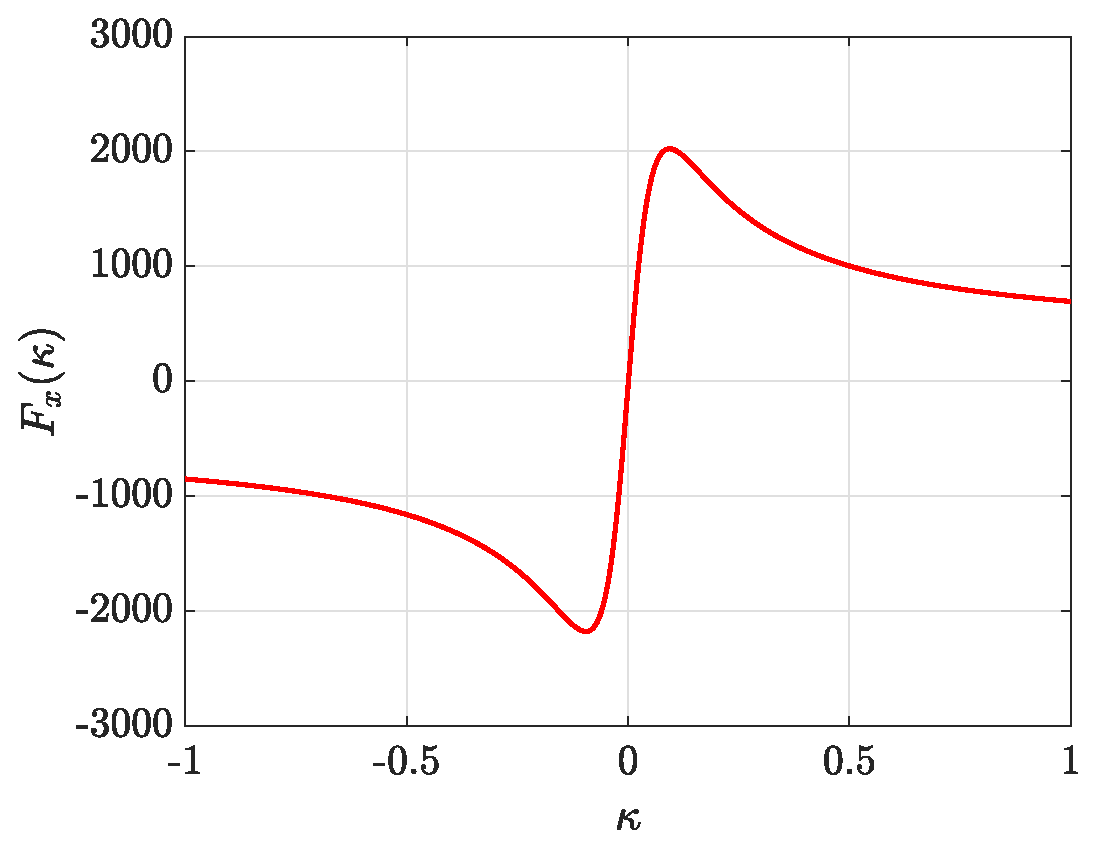
\includegraphics[scale=0.5]{ex1/e-11.eps}
        \centering
        \caption{$\fxz$ as a function of slip}
        \end{figure}

When $\kappa$ (longitudinal slip) increases, $\fx$\ grows until it reaches a saturation limit. Furthermore, the slip zone grows, and the adherence area decreases. That means, the total tire force $\fx$\ keeps growing until it reaches a peak and a saturation limit as shown in the graph below. $\kappa$ (longitudinal slip) is positive when the tire is accelerating, negative during braking, and reaches -1 when the wheel locks.
        \begin{figure}[ht]
        \includegraphics[scale=1]{ex1/e-12.png}
        \centering
        \caption{Slip and adherence forces}
        \end{figure}


\textbf{Q. If you were supposed to design a traction control system for maximizing vehicle longitudinal acceleration, which would be the target value of longitudinal slip $\kappa$ that you would try to achieve?}

Acceleration is directly proportional to the force [F=ma] if the mass is constant. If I want to maximize the vehicle longitudinal acceleration, I would need to maximize the longitudinal force [$\fx$]. $\fx$\ is highest at the saturation limit, which in this example happens at slip $\kappa$ = 0.094, and yields an $\fx$\ of 2022.99 N.

\textbf{Q. Assuming that wheel rotational speed is $\omega$ = 70 rad/s, tire effective rolling radius is R$_{e}$ = 0.2 m, while the longitudinal component of tire contact point speed $\vcx$\ = 13 m/s, compute the longitudinal slip $\kappa$. In these conditions, is the wheel accelerating, braking or is it in pure rolling? Compute also the corresponding longitudinal tire force $\fxz$}

Using Matlab, the calculated longitudinal slip $\kappa$ = 0.0769 and the calculated longitudinal force $\fx$\ is = 1990.65 N. the longitudinal slip is positive ($>$0), which means that the wheel is accelerating.

\textbf{Q. Compute the cornering stiffness Cf$\kappa$, that is the derivative for $\kappa$ = 0 of the $\fxz$. Up to which value of $\kappa$ is the linear approximation of Pacejka curve acceptable?}

The cornering Stiffness Cf$\kappa$ is equal to the derivative of the longitudinal force with respect to the longitudinal slip when the longitudinal slip is equal to zero. This means its equal to the slope at the origin (x=y=0) or equal to BCD function as shown in Figure \ref{co-st}. The calculated cornering stiffness is Cf$\kappa$ = 47909.4

        \begin{figure}[ht]
        \includegraphics[scale=1.2]{ex1/e-13.png}
        \centering
        \caption{cornering stiffness as a linear approximation}
        \label{co-st}
        \end{figure}
        
The linear approximation allows to neglect the complex Pacejka Magic Formula, but it is valid only for small $\kappa$. At $\kappa$ = 0.02, the percent difference is already at 10\% as shown in Figure \ref{pd-p}.

        \begin{figure}[ht]
        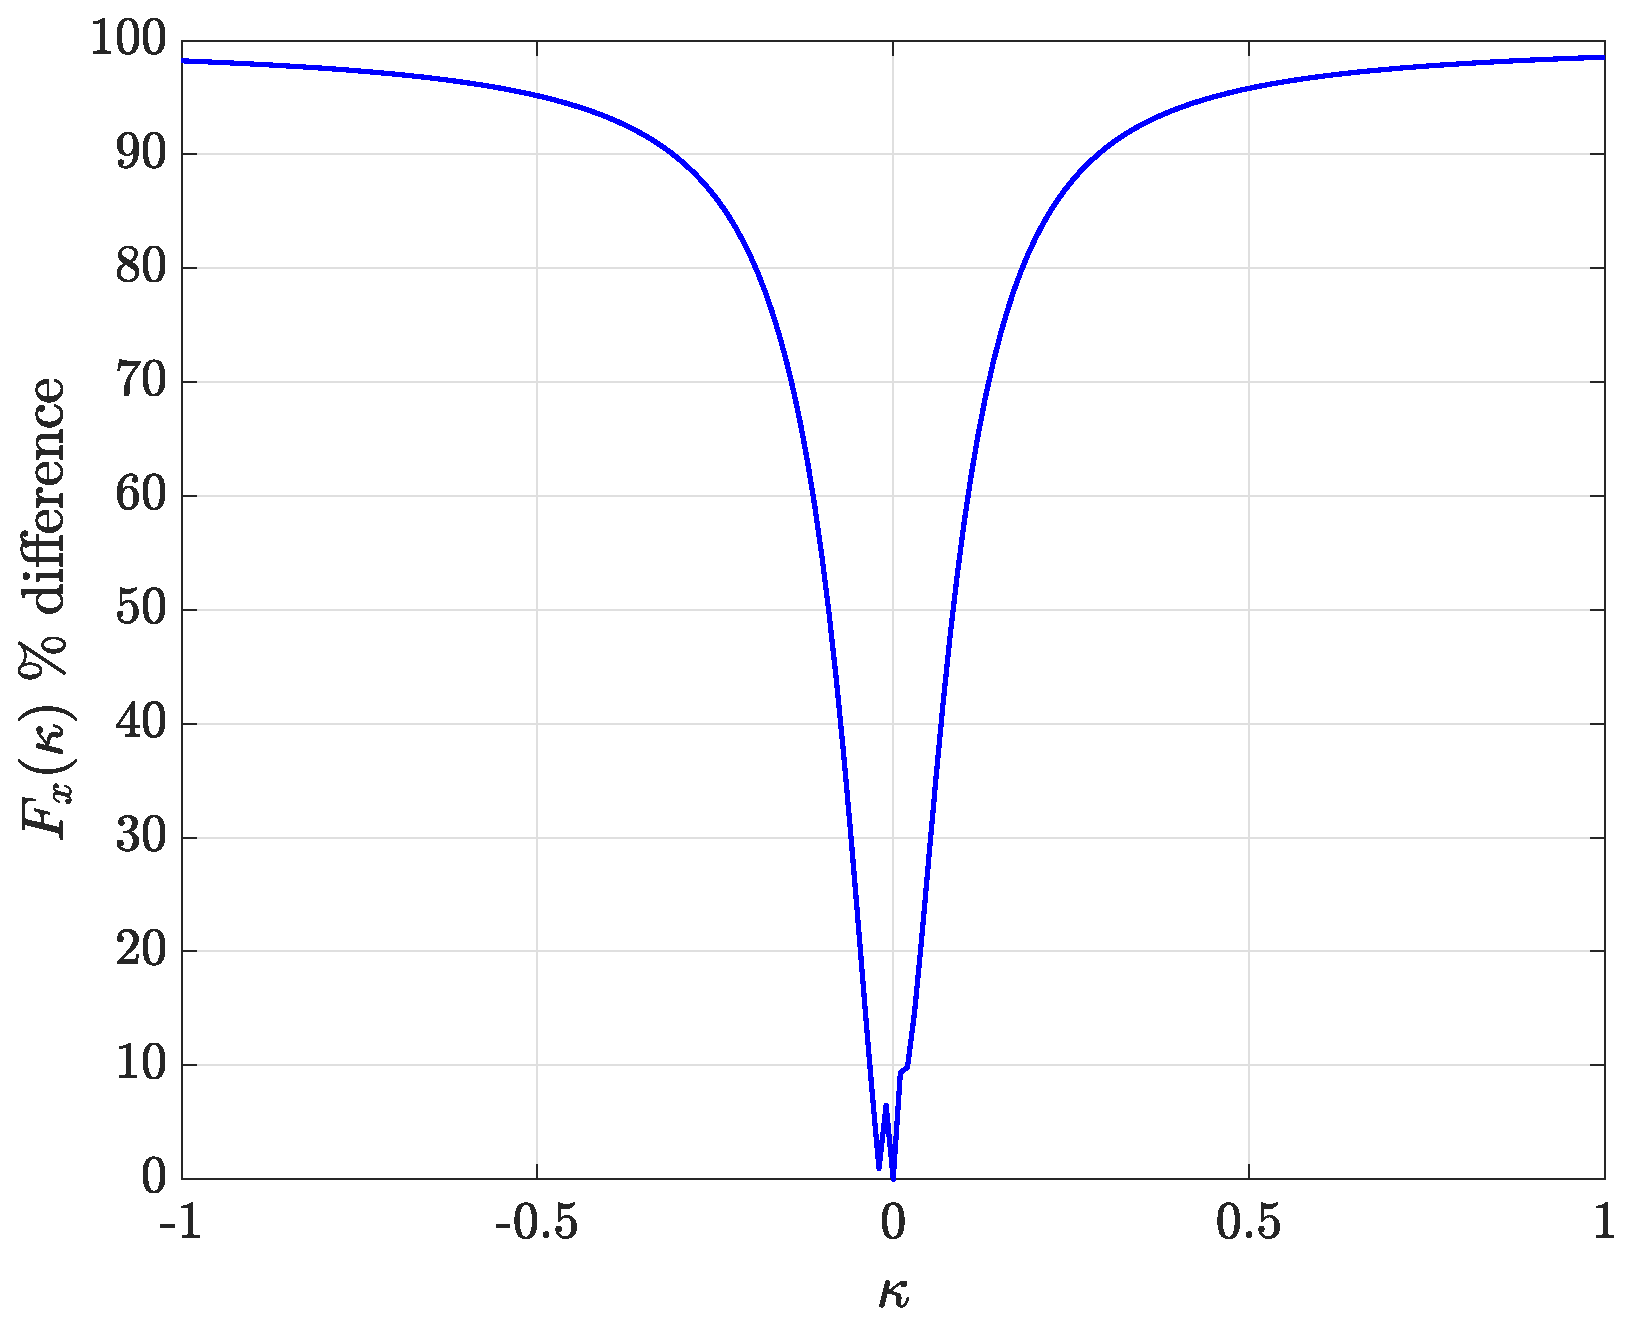
\includegraphics[scale=0.5]{ex1/e-15.eps}
        \centering
        \caption{\% difference in $\kappa$ using linear approximation vs Pacejka formula}
        \label{pd-p}
        \end{figure}

\newpage

\section{Exercise 2 - Combined Slip}

\textbf{Q. Assume that the tire contact point velocity components along the tire x and y axes are $\vcx$\ = 15 m/s and $\vcy$\ = −1.3 m/s, respectively. Calculate the side slip angle $\alpha$. Moreover, compute the combined tire force $\fx$\ using this value of $\alpha$, for a longitudinal slip $\kappa$ = 0.08.}

Alpha can be calculated using the practical slip approach:

\begin{equation}\label{eq:1.1} % add * after equation for unnumbered equations
    \mbox{side slip angle  }  \alpha = - \arctan(\frac{\vsy}{\vcx}) = - \arctan(\frac{\vcy}{\vcx})
\end{equation}

Using equation \ref{eq:1.2} to calculate $\gxa$\ (weighing function). Once calculated, $\fxz$\ can now be multiplied by $\gxa$\ (weighing function) to get the combined tire force $\fx$.

\begin{equation}\label{eq:1.2} % add * after equation for unnumbered equations
    \gxa = - \dxa \cos(\cxa \arctan(\bxa(\alpha + \shxa))
\end{equation}{\vspace{-4em}}

\begin{equation}\label{eq:1.3} % add * after equation for unnumbered equations
    \fxz = \dx \sin(\cx \arctan(\bx \kx - \ex(\bx \kx - \arctan(\bx \kx)))
\end{equation}{\vspace{-4em}}

\begin{equation}\label{eq:1.4} % add * after equation for unnumbered equations
    \fx = \gxa \fxz
\end{equation}

Using Matlab to calculate the side slip angle $\alpha$ and combined tire force:

{\centering\fbox{\begin{minipage}{20em}
calculated side slip alpha = 0.086451 \\
calculated weighing function = 0.724417 \\
calculated combined force $\fx$\ = 1450.424623
\end{minipage}}\par}

\textbf{Q. Plot the combined longitudinal tire force $\fx$\ as a function of $\kappa$ $\in$ [−1, 1], for the following levels of side slip angle $\alpha$ = \{0, 2, 4, 6, 8\} degrees. Which comments can you make about the 5 curves obtained in this way? Finally, plot the weighting function $\gxa$\ as a function of $\kappa$ $\in$ [−1, 1] for each of the previously defined values of $\alpha$, and briefly comment also these 5 curves.}

Figure \ref{clf} shows plots obtained for the combined longitudinal force $\fx$\ for each side slip angle as a function of the longitudinal slip $\kappa$. The maximum combined longitudinal force $\fx$\ keeps decreasing with higher side slip $\alpha$.\newpage

        \begin{figure}[ht]
        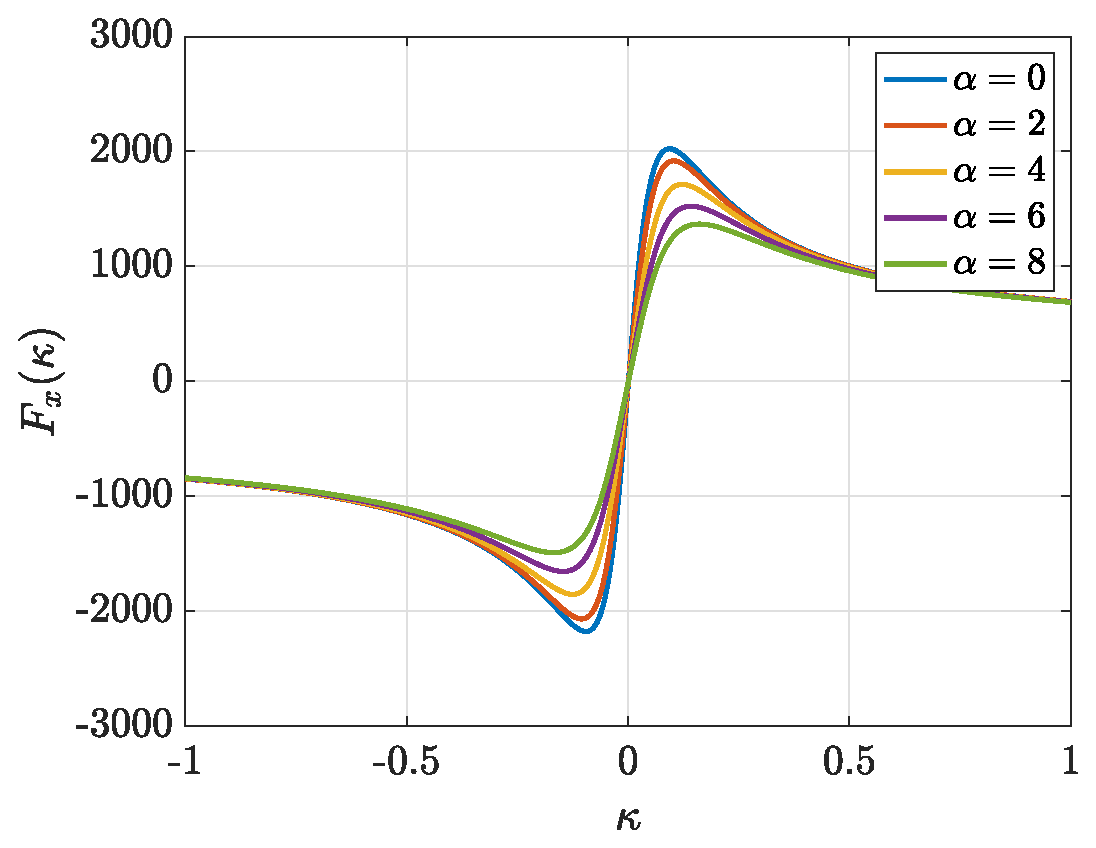
\includegraphics[scale=0.5]{ex1/e-16.eps}
        \centering
        \caption{combined longitudinal force $\fx$\ as a function of $\kappa$}
        \label{clf}
        \end{figure}

Figure \ref{wf} shows the plots obtained for the weighing function $\gxa$\ for each side slip angle as a function of the longitudinal slip $\kappa$. Higher side slip $\alpha$ decreases the weighing function, which in effect decreases the combined longitudinal force $\fx$. The effect of the weighing function is quite more potent around $\kappa$ = 0, and that effect decreases the further away we are from it.

        \begin{figure}[ht]
        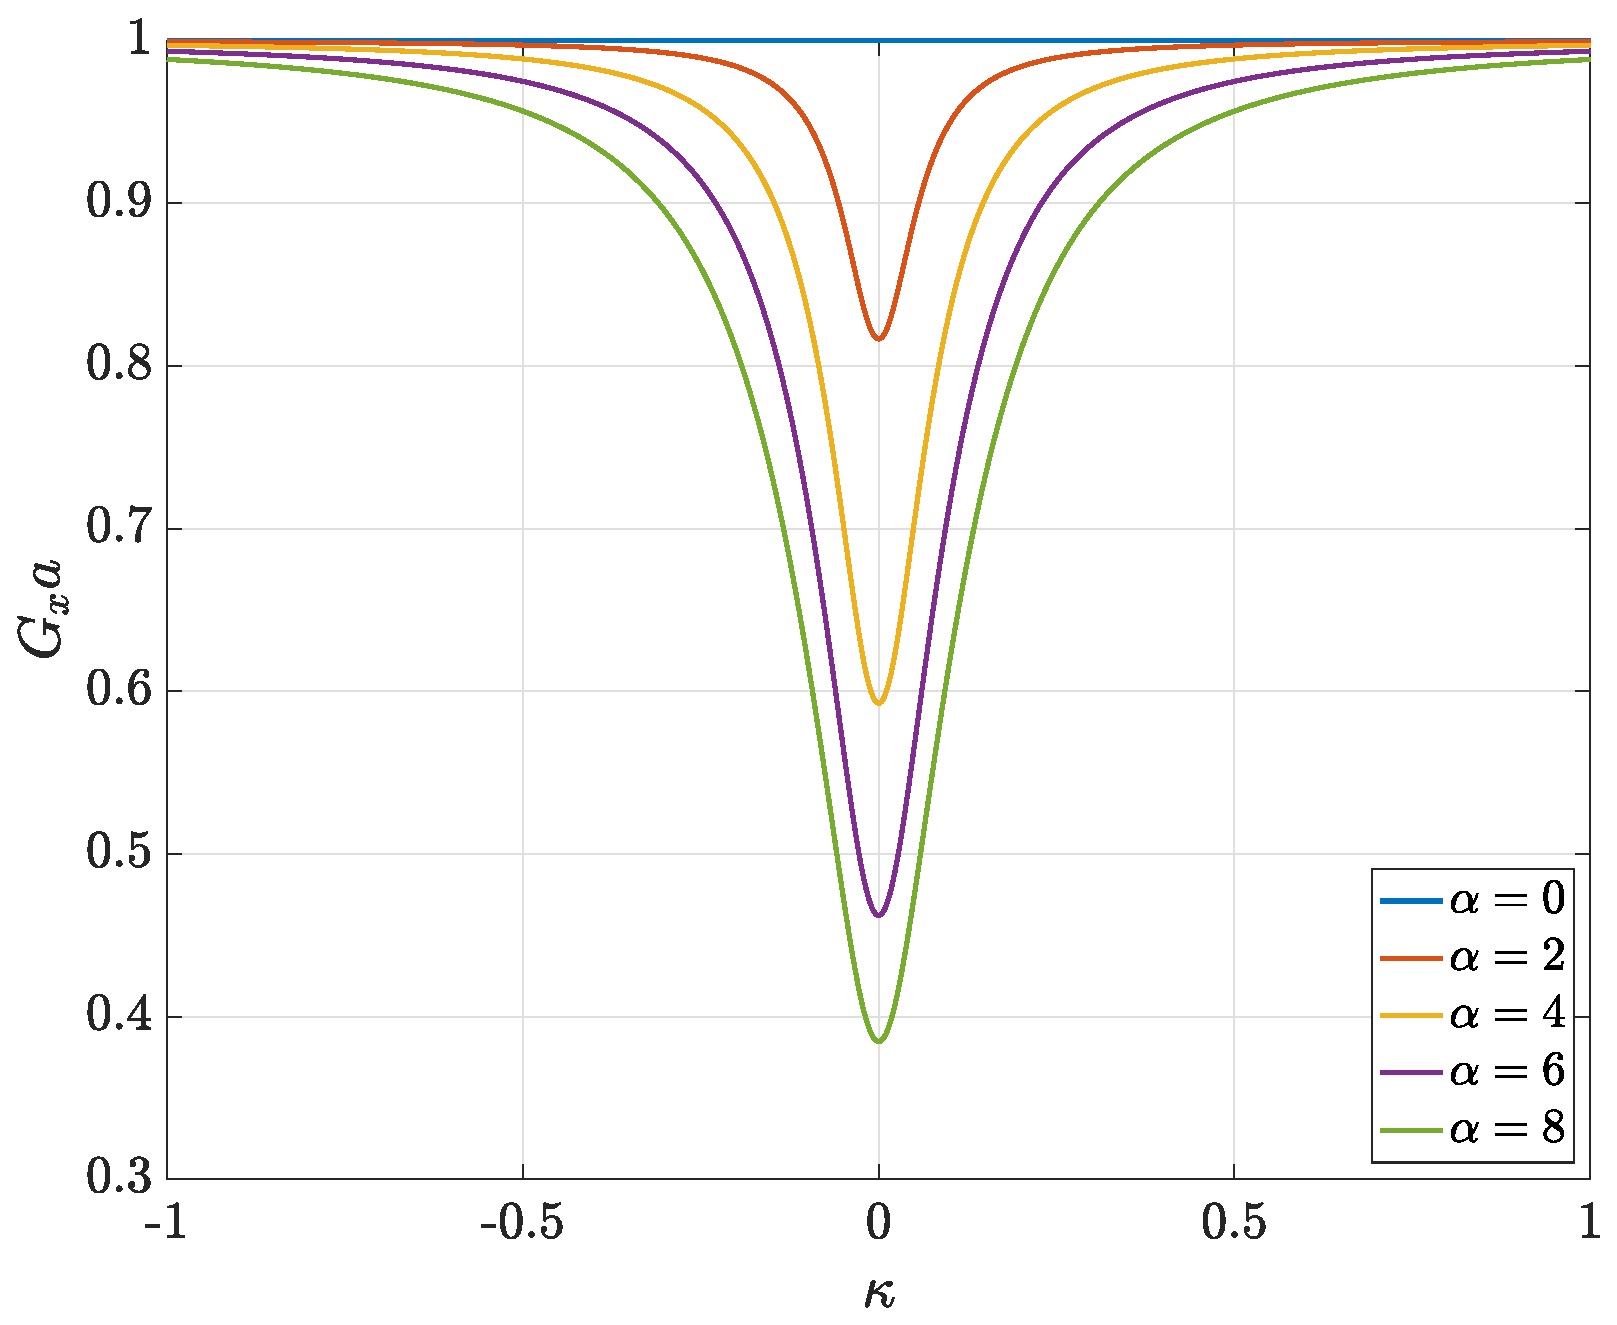
\includegraphics[scale=0.5]{ex1/e-17.eps}
        \centering
        \caption{Weighing function $\gxa$\ as a function of $\kappa$}
        \label{wf}
        \end{figure}

\documentclass[../main.tex]{subfiles}
\begin{document}

\subsection*{Exercise 1 – Understanding tire data}
\textbf{Q. Plot the raw data in different graphs, specifically focusing on $\kappa$, $\alpha$, $\gamma$, $\fz$\ and pressure $P$. Comment on what you see. What is, according to you, the main target of these tests?}

        \begin{figure}[ht]
        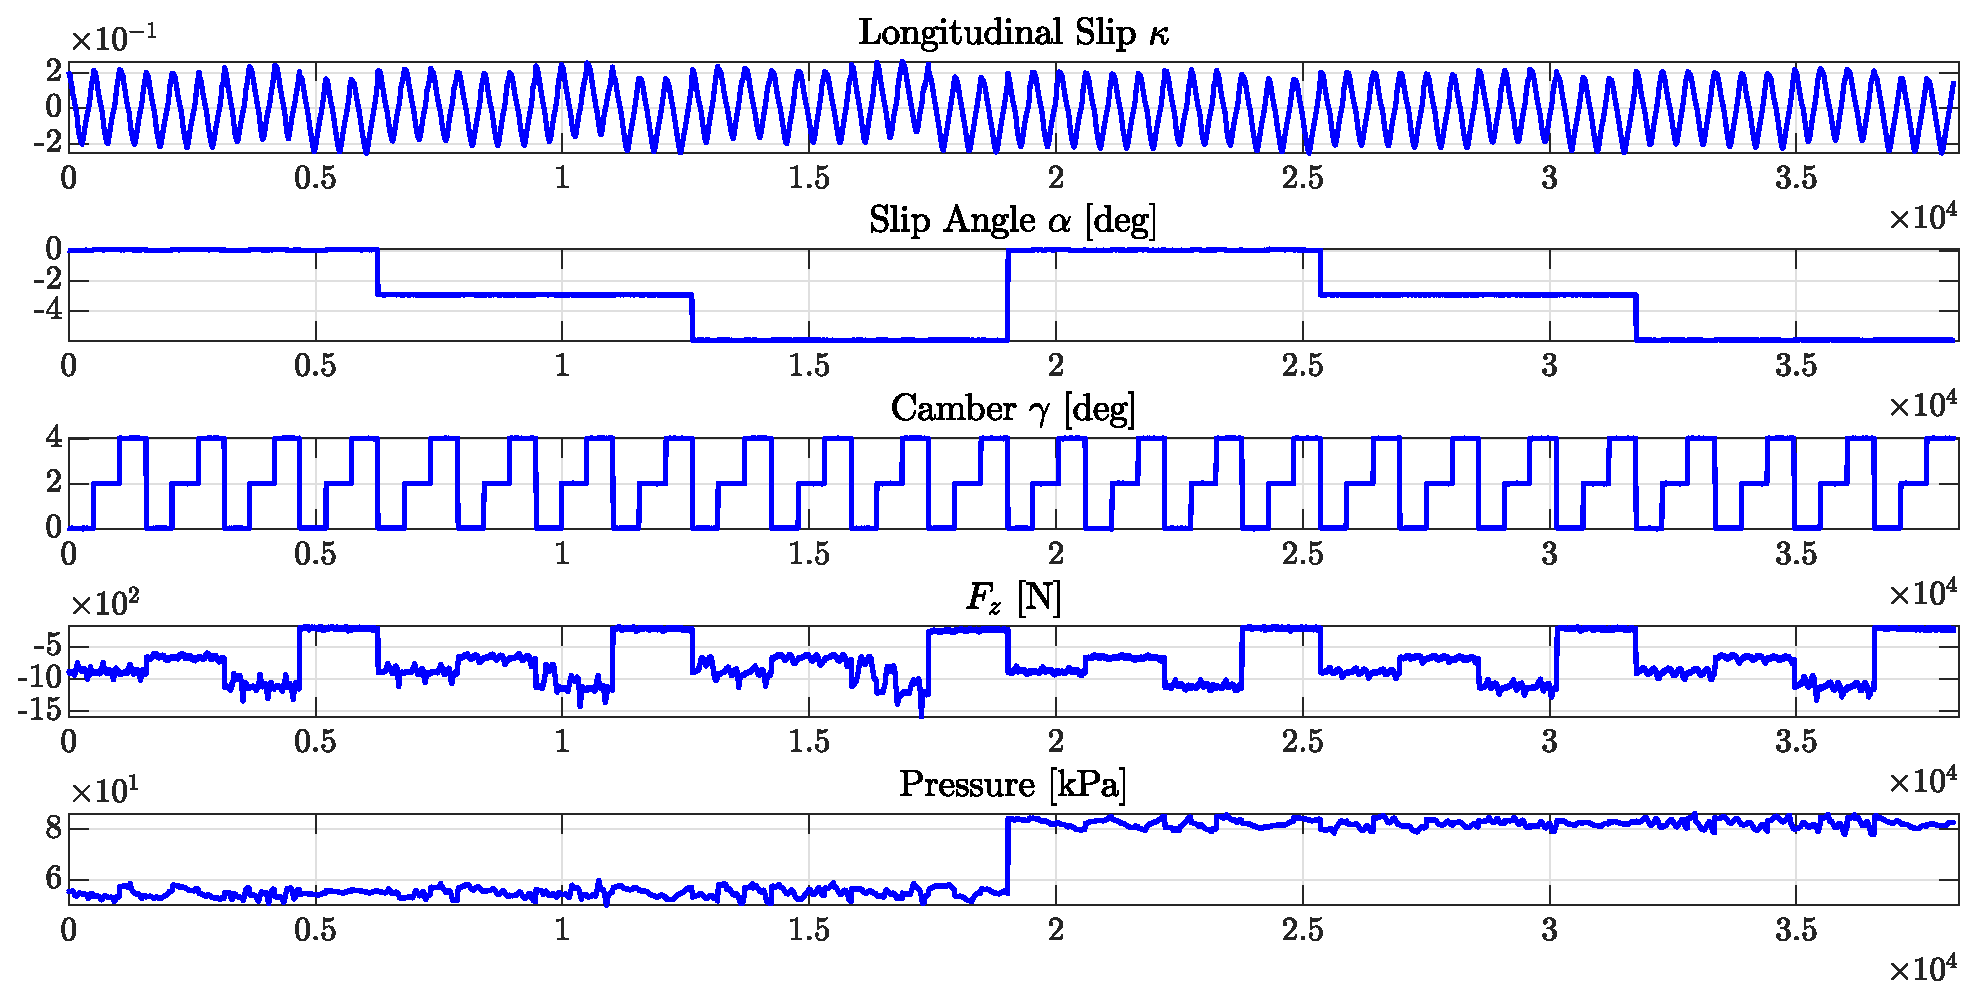
\includegraphics[scale=0.4]{ex2/ex-21.eps}
        \centering
        \caption{raw data}
        \label{rd}
        \end{figure}

From the five plotted variables if Figure \ref{rd}, it appears that the slip angle, camber, vertical force, and pressure are all showing repeat patterns. That means that those four variables are controlled to measure and test the longitudinal slip $\kappa$.

\textbf{Q. Focus on the data with $\alpha$ =0 and $\gamma$ =0, and plot the curves $\fx$\ vs $\kappa$ for each of the 4 vertical loads $\fz$\ used in the experiments. Plot the 4 curves on the same graph, with different colors. Comment on what you see.}

        \begin{figure}[ht]
        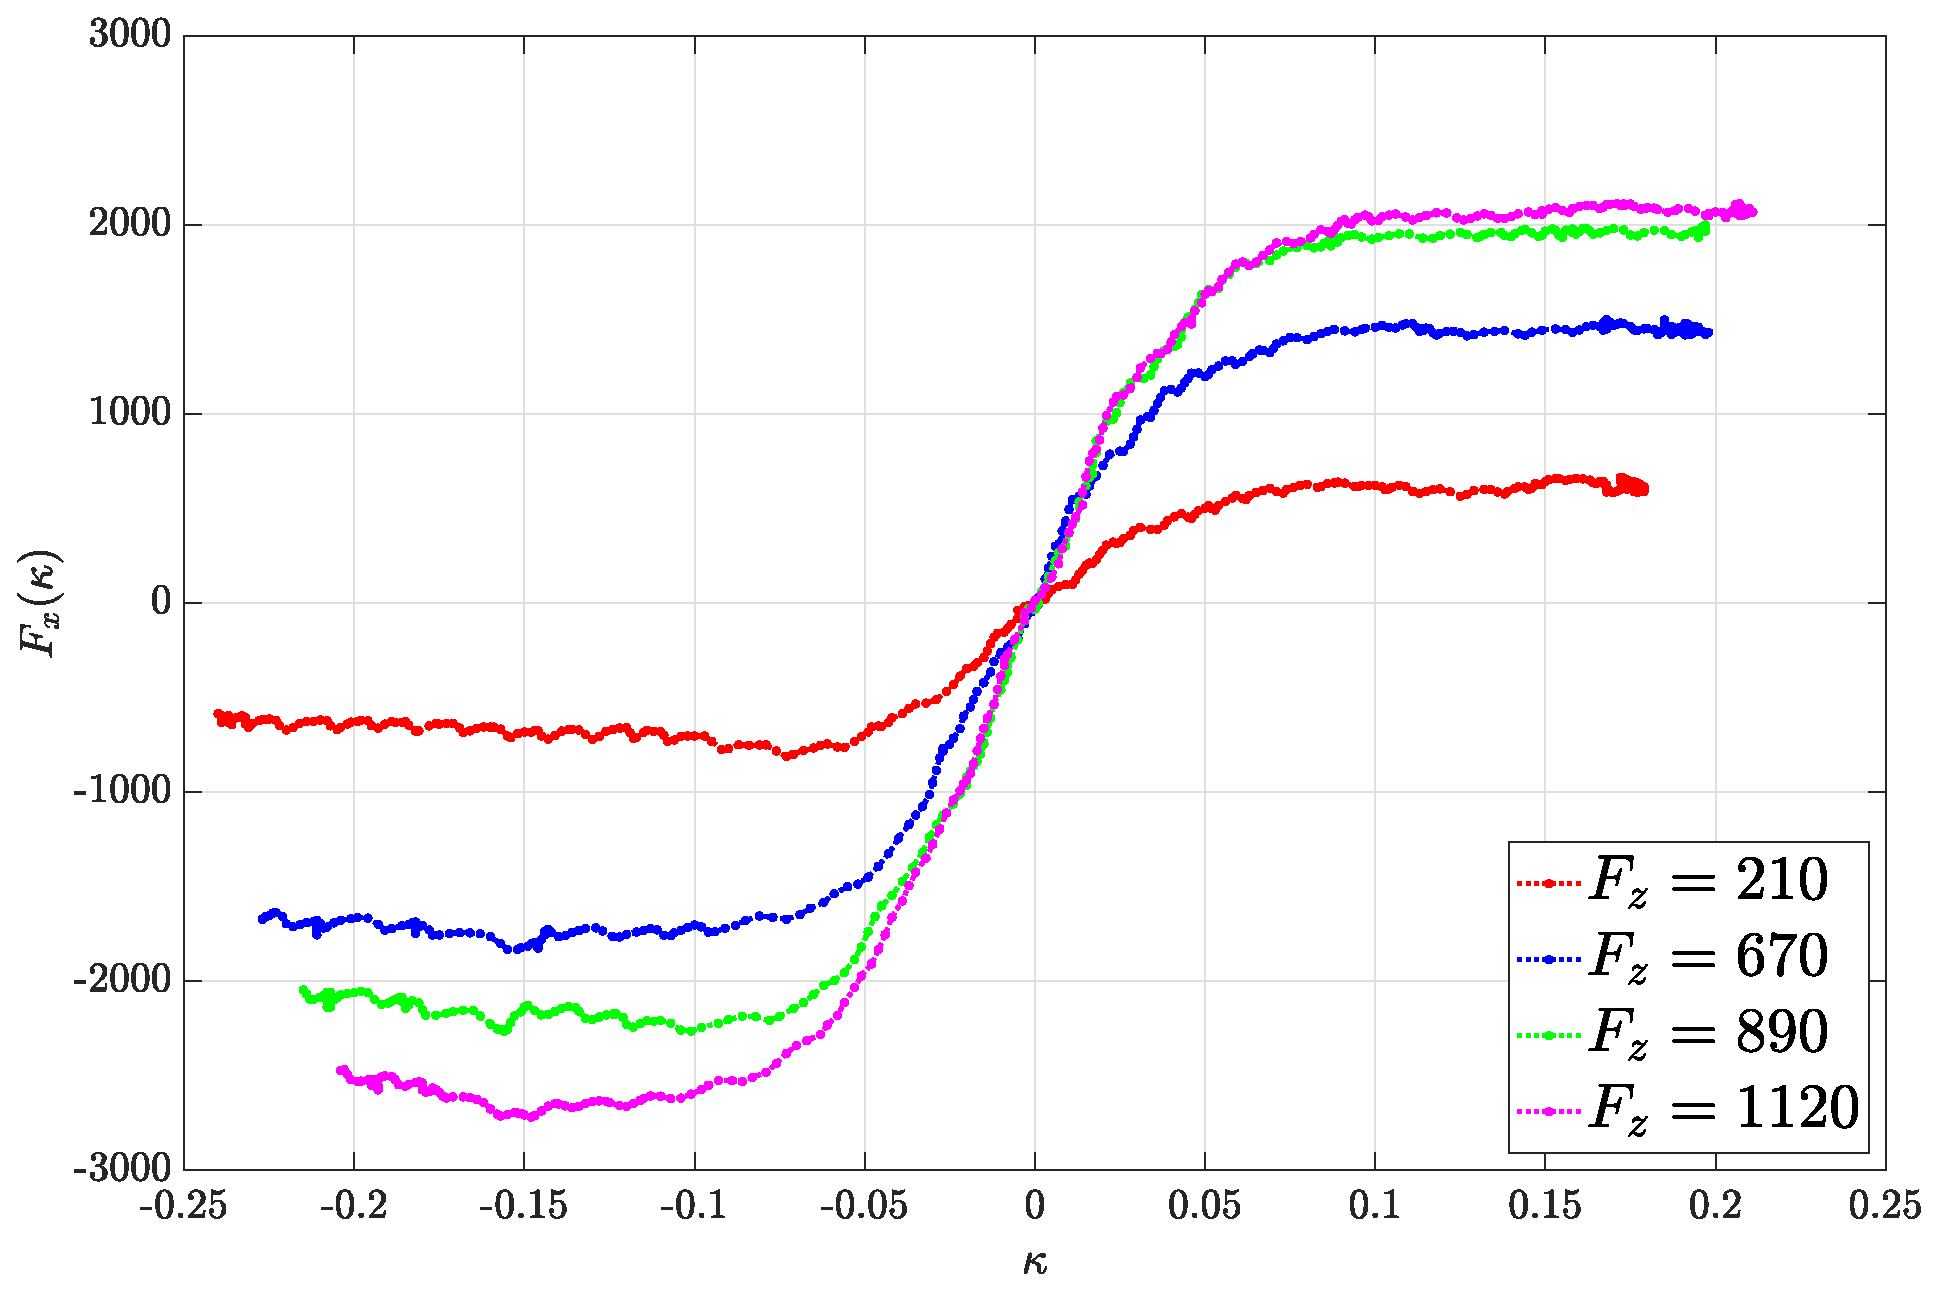
\includegraphics[scale=0.35]{ex2/ex-22.eps}
        \centering
        \caption{$\kappa$ vs $\fx$\ based on vertical force}
        \label{lsvlf}
        \end{figure}

Figure \ref{lsvlf} suggests that the Longitudinal Force $\fx$\ increases with the vertical force $\fz$. There is some dependency on the vertical force. If you double the vertical force, it does not mean the longitudinal force will double. In some parts there is a linear dependency, but in others it is not the case.

\textbf{Q. Focus on the data with $\gamma$ =0 and $\fz$\ = 150 lbf $\approx$ 670N, and plot the curves $\fx$\ vs $\kappa$ for each of the 3 side slip angles $\alpha$ used in the experiments. Plot the 3 curves on the same graph, with different colors. Comment on what you see.}

The Longitudinal Force $\fx$\ in Figure \ref{lsvlfv} shows an inverse relationship with the side slip angle. 
        \begin{figure}[ht]
        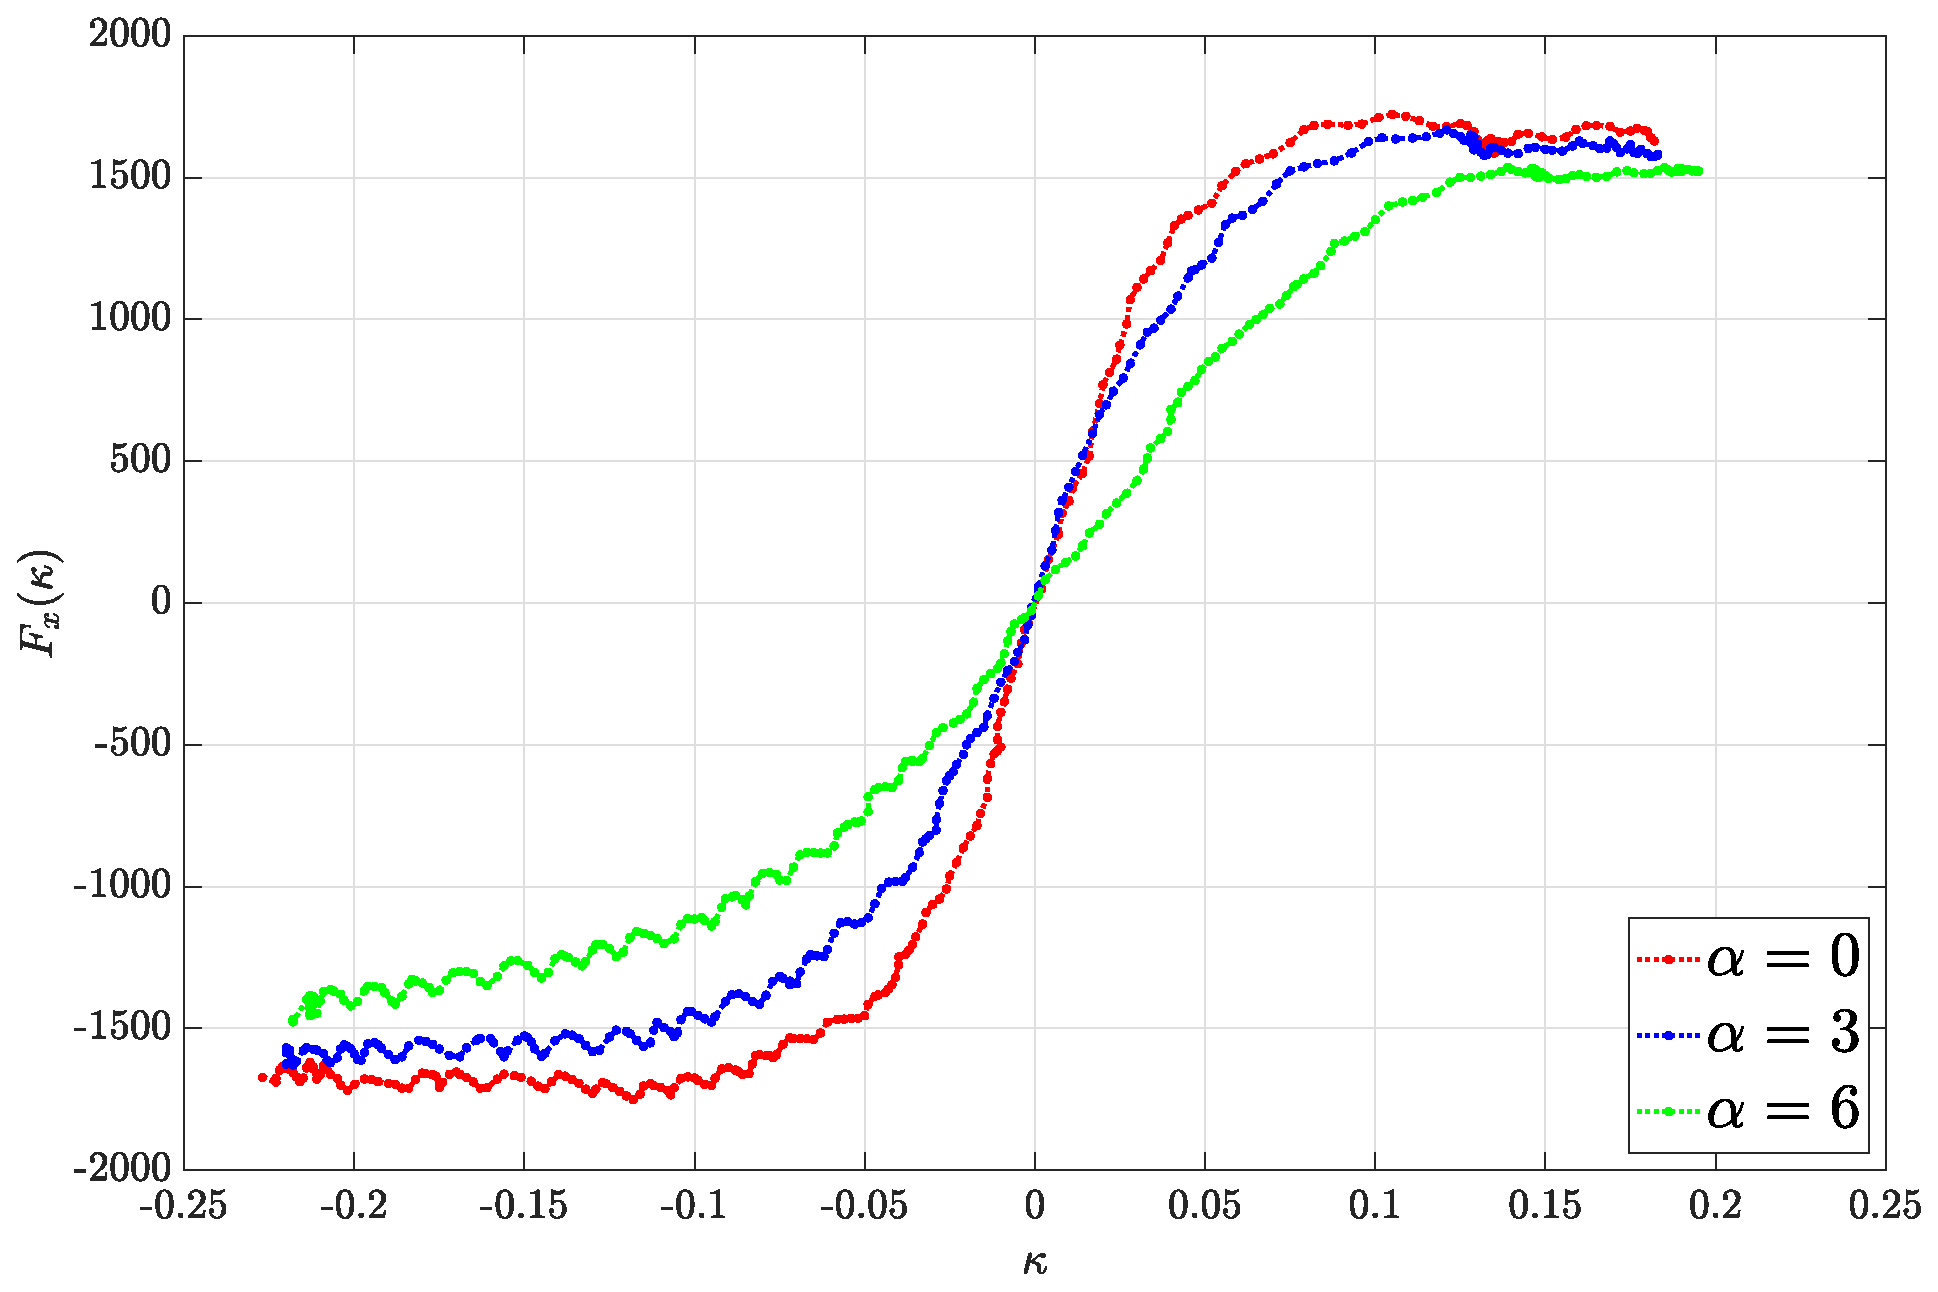
\includegraphics[scale=0.35]{ex2/ex-23.eps}
        \centering
        \caption{$\kappa$ vs $\fx$\ at vertical force = 670 based on slip angle}
        \label{lsvlfv}
        \end{figure}

\subsection*{Exercise 2 - Fitting tire data}

\textbf{Q. First consider the data with $\fz$\ = $\fzz$\ =890N, $\gamma$ =0 and $\alpha$ =0, and fit the coefficients X1 = \{$\pcxo$, $\pdxo$, $\pexo$ , $\pexf$, $\pkxo$, $\phxo$, $\pvxo$\}. Build a function $resid pure \fx$ that calculates the pure longitudinal force $\fxz$\ and the residuals. Plot the fitted curve $\fx$\ vs $\kappa$ that you obtained in these nominal conditions, together with the raw data.}

        \begin{figure}[ht]
        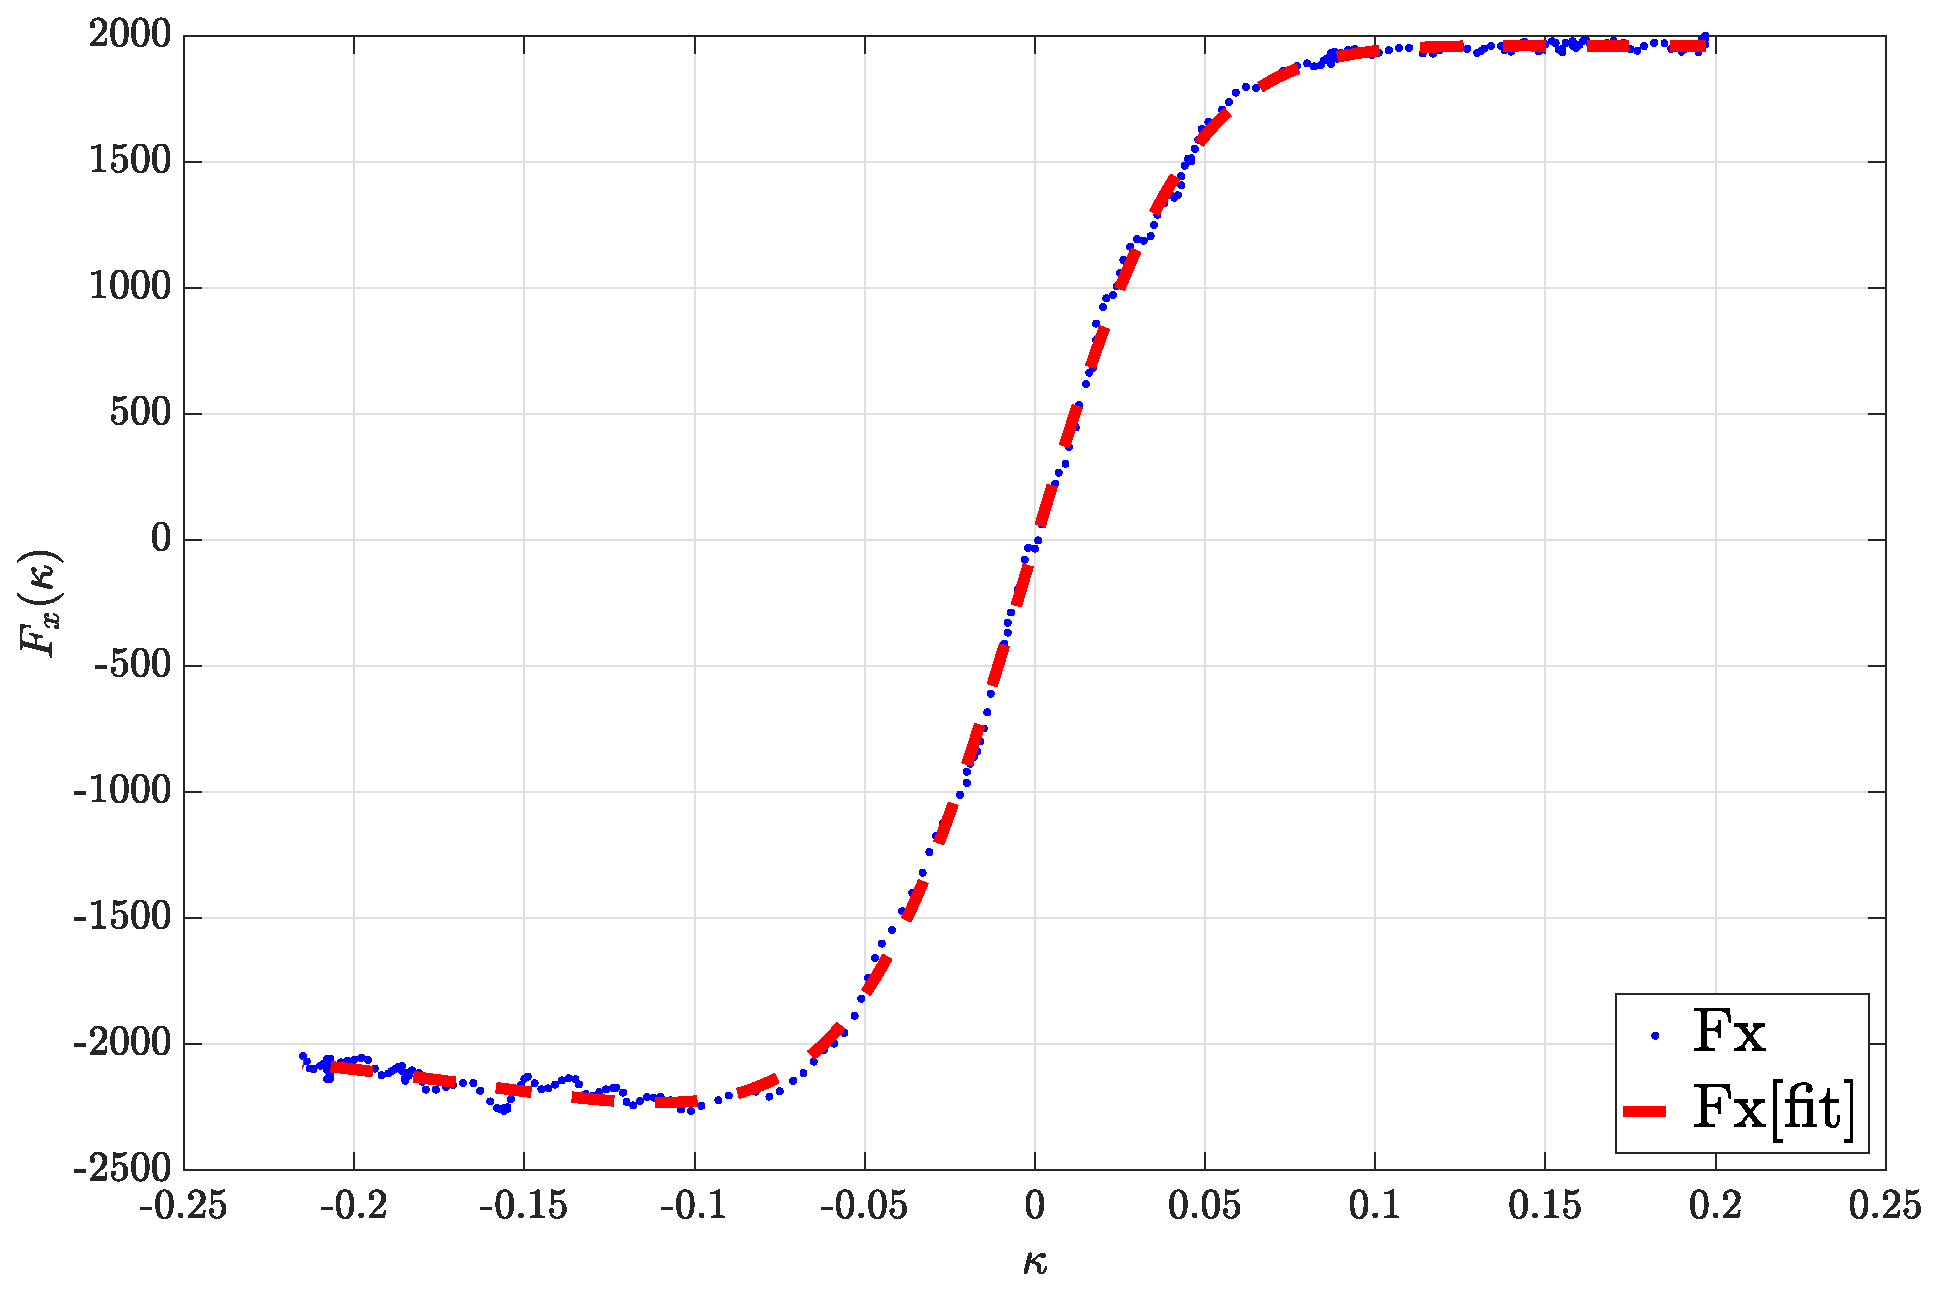
\includegraphics[scale=0.35]{ex2/ex-24.eps}
        \centering
        \caption{Fitted $\fxz$\ after optimizing first 7 parameters compared to test data vs $\kappa$}
        \label{faopt}
        \end{figure}

In Figure \ref{faopt}, the data was filtered based on the following criteria: $\fzz$\ = 890, $\alpha$\ = 0, $\gamma$\ = 0 and $P$ = 82kPa. The first 7 coefficients were optimized using the $fmincon$ function in Matlab. The 7 coefficients initial guess vector was chosen randomly. The initial guess vector has proven to be quite important as running the code multiple times showed a curve that did not fit the data at all, which means the optimizer was stuck at a local minima. However, most of the time the initial guess gave a very good fit that converged to the correct global minima. 


\textbf{Q. Now consider the data with the 4 different values of $\fz$, but still $\gamma$ = 0 (and $\alpha$ = 0). This enables the fitting of the parameters: X2 =\{$\pdxt$,$\pext$,$\pextt$,$\phxt$,$\pkxt$,$\pkxtt$,$\pvxt$\}. You can build another function so as to use the optimal parameters X1,opt found before for the coefficients already computed. Plot the fitted and raw curves $\fxz$\ vs $\kappa$ for the 4 values of $\fz$\ and comment the results.}

\end{document}
\documentclass[../main.tex]{subfiles}
\graphicspath{{\subfix{../images/}}}
\newcommand{\vcx}{\upsilon_{Cx}}
\newcommand{\vcy}{\upsilon_{Cy}}
\newcommand{\vsy}{\upsilon_{sy}}

\newcommand{\fxz}{F_{x0}}
\newcommand{\fx}{F_{x}}
\newcommand{\fy}{F_{y}}
\newcommand{\fzz}{F_{z0}}
\newcommand{\fz}{F_{z}}
\newcommand{\fa}{F_{A}}

\newcommand{\ay}{a_{y}}

\newcommand{\mz}{M_{z}}

\newcommand{\uz}{u_{0}}
\newcommand{\ts}{T_{s}}
\newcommand{\tf}{T_{f}}

\newcommand{\bx}{B_{x}}
\newcommand{\cx}{C_{x}}
\newcommand{\dx}{D_{x}}
\newcommand{\ex}{E_{x}}
\newcommand{\gxa}{G_{xa}}
\newcommand{\bxa}{B_{xa}}
\newcommand{\cxa}{C_{xa}}
\newcommand{\dxa}{D_{xa}}

\newcommand{\shxa}{S_{Hxa}}
\newcommand{\kx}{\kappa_{x}}
\newcommand{\svx}{S_{Vx}}
\newcommand{\pcxo}{p_{Cx1}}
\newcommand{\pdxo}{p_{dx1}}
\newcommand{\pexo}{p_{Ex1}}
\newcommand{\pexf}{p_{Ex4}}
\newcommand{\pkxo}{p_{Kx1}}
\newcommand{\phxo}{p_{Hx1}}
\newcommand{\pvxo}{p_{Vx1}}

\newcommand{\pdxt}{p_{dx2}}
\newcommand{\pext}{p_{Ex2}}
\newcommand{\pextt}{p_{Ex3}}
\newcommand{\pkxt}{p_{Kx2}}
\newcommand{\pkxtt}{p_{Kx3}}
\newcommand{\phxt}{p_{Hx2}}
\newcommand{\pvxt}{p_{Vx2}}
\begin{document}
\subsection*{Exercise 1 – Understanding vehicle data}

\textbf{Q. Plot lateral and longitudinal velocity}

        \begin{figure}[ht]
        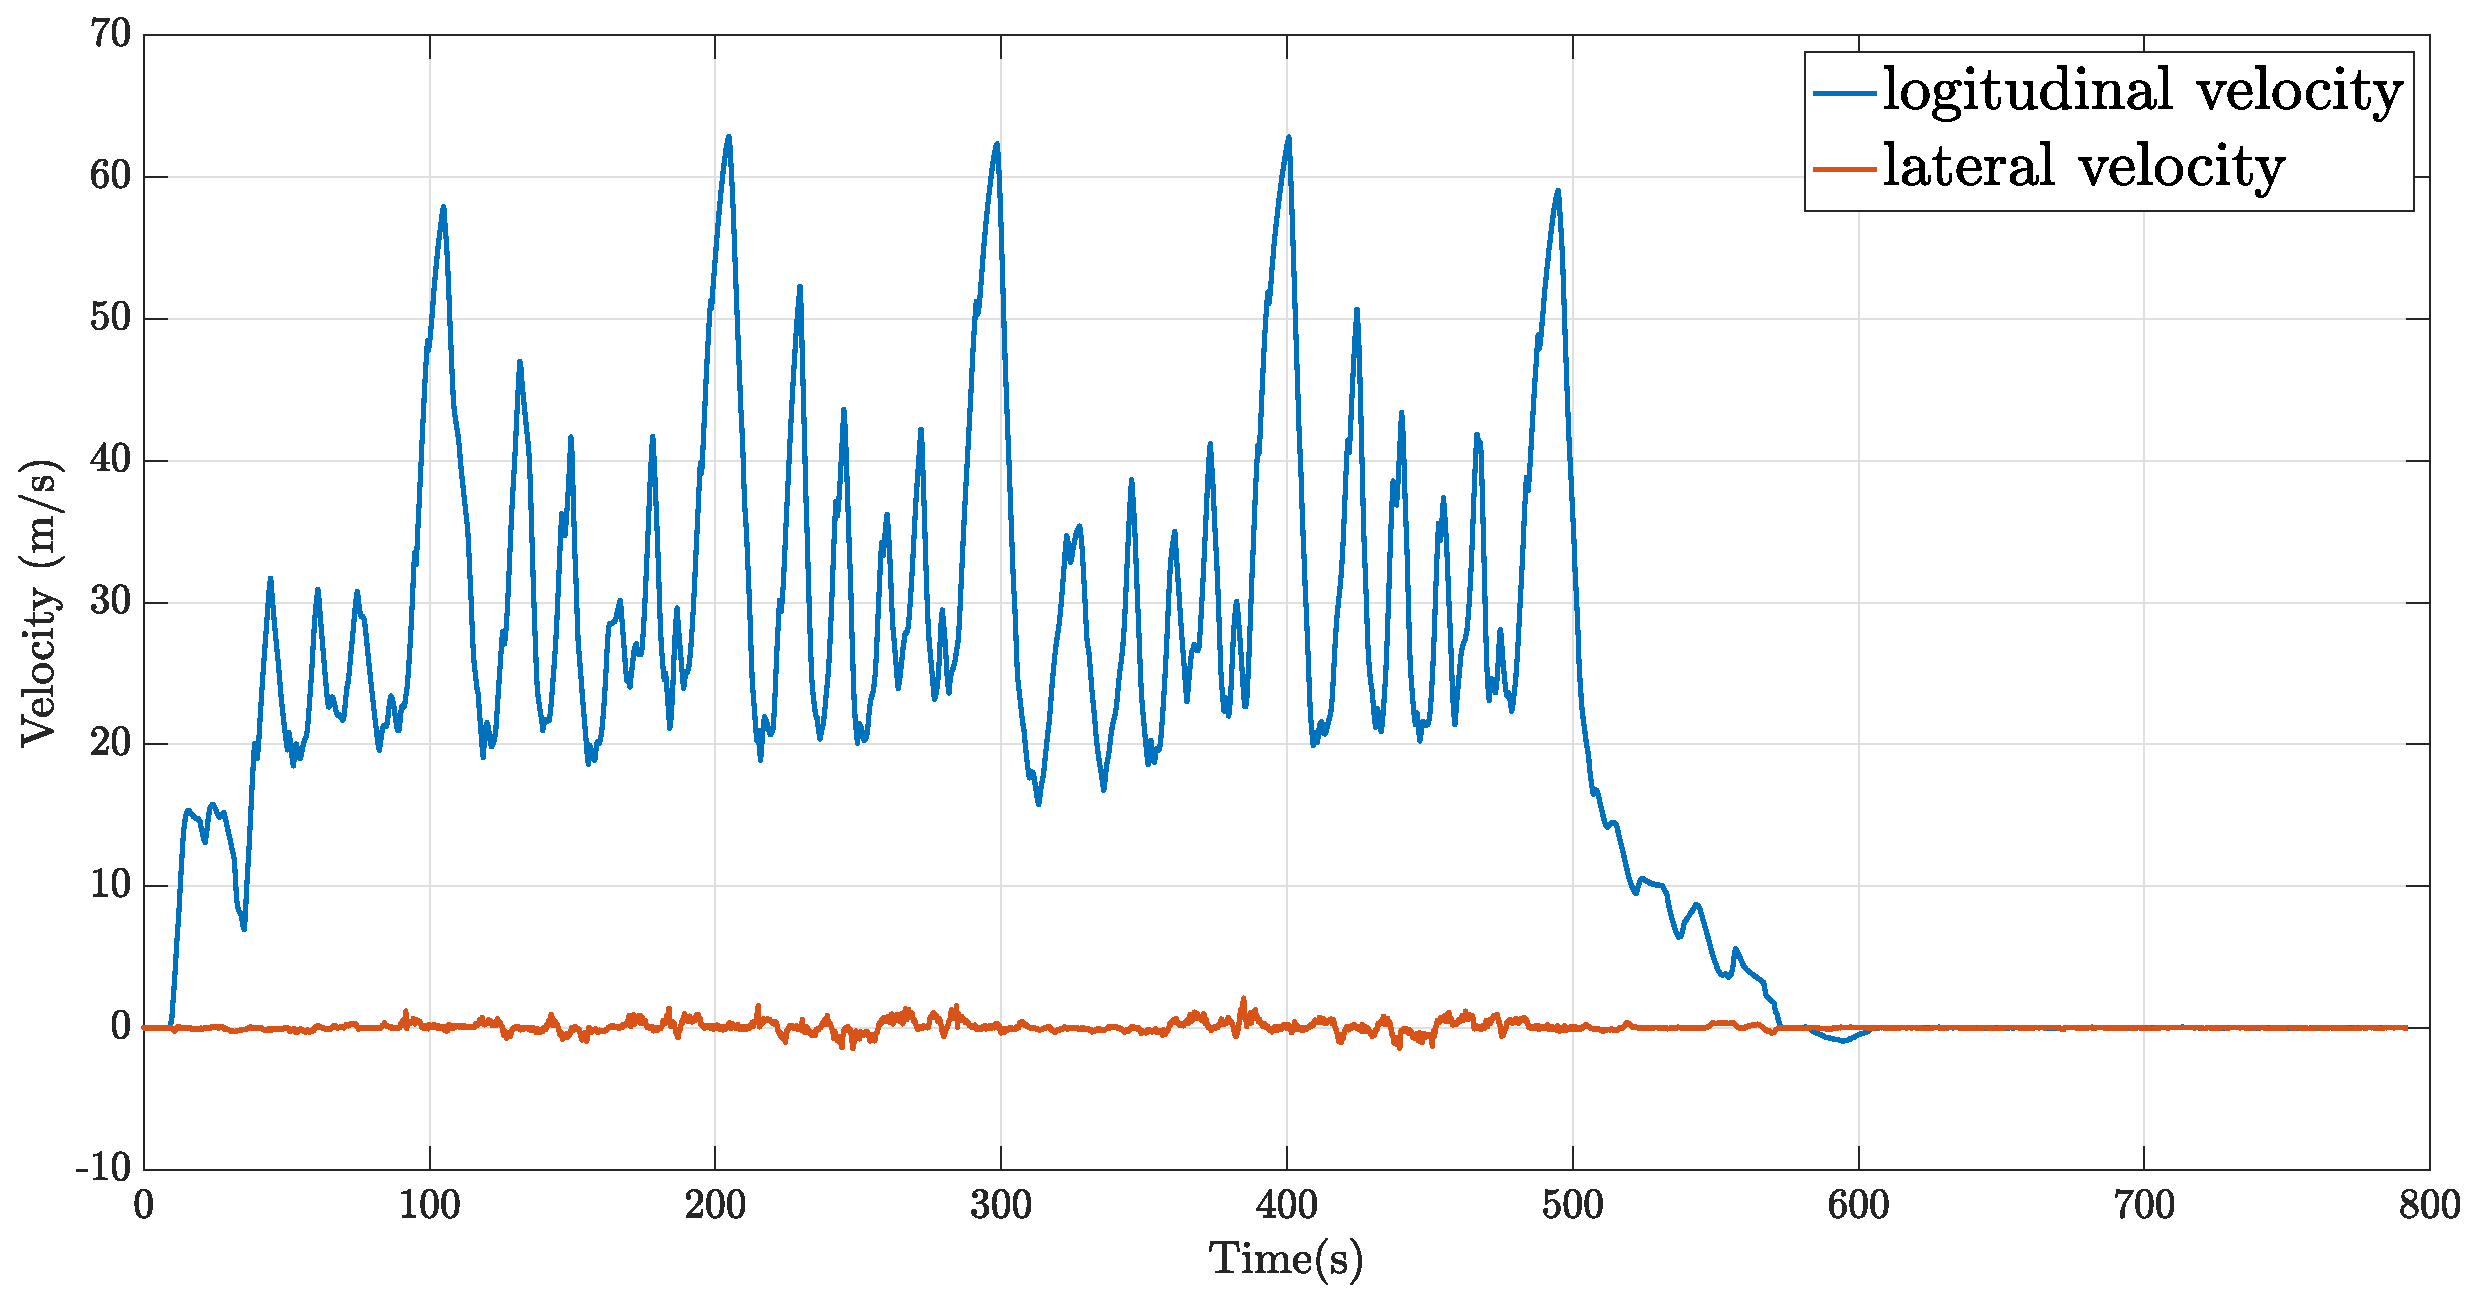
\includegraphics[scale=0.35]{ex3/ex-31.eps}
        \centering
        \caption{lateral and longitudinal velocity vs. time}
        \label{llv}
        \end{figure}
        
From Figure \ref{llv}, the magnitude of the longitudinal velocity is higher than the lateral velocity.

\textbf{Q. Evaluate the longitudinal speed using the Hall-effect wheel speed sensors and compare the data with the INS data}

        \begin{figure}[ht]
        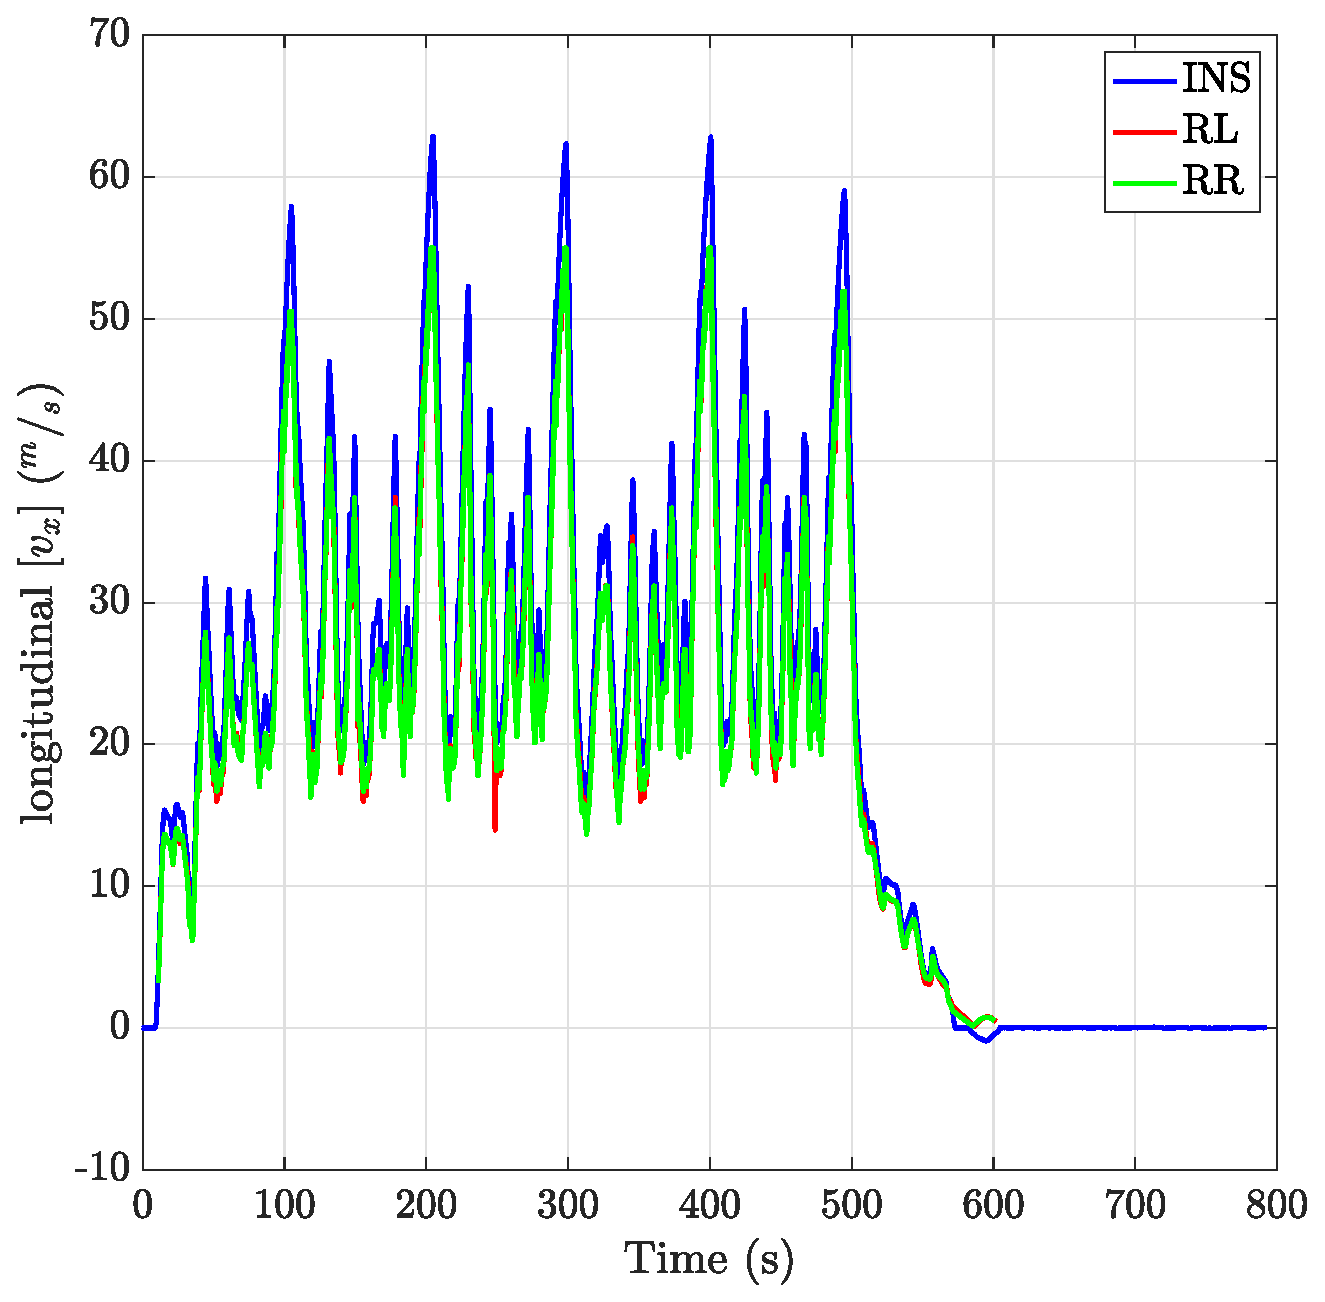
\includegraphics[scale=0.3]{ex3/ex-32.eps}
        \centering
        \caption{longitudinal speed vs time [INS and hall effect sensors RL and RR]}
        \label{lsvt}
        \end{figure}
 
The longitudinal speed for the vehicle was calculated using the hall effect sensor data. Only the rear wheels [left and right] were used for the calculation. That is because they do not have a torque applied on them and they are ``free rolling”. Every change in voltage [tick] means a full revolution of the tire. The time difference between 2 ticks was calculated [$\overline{T}$] and used in equation \ref{eq:5} to estimate the longitudinal speed [Where c is the wheel circumference]:

\begin{equation}\label{eq:5}
    \upsilon_{wheel} = \frac{c}{\overline{T}}
\end{equation}

The INS velocity is sometimes bigger than the hall effect calculated speeds, especially during braking [partial wheel lock]. There is no obvious difference between them.

\textbf{Q. Evaluate the lateral acceleration using the relation with the yaw-rate and the longitudinal speed.}

        \begin{figure}[ht]
        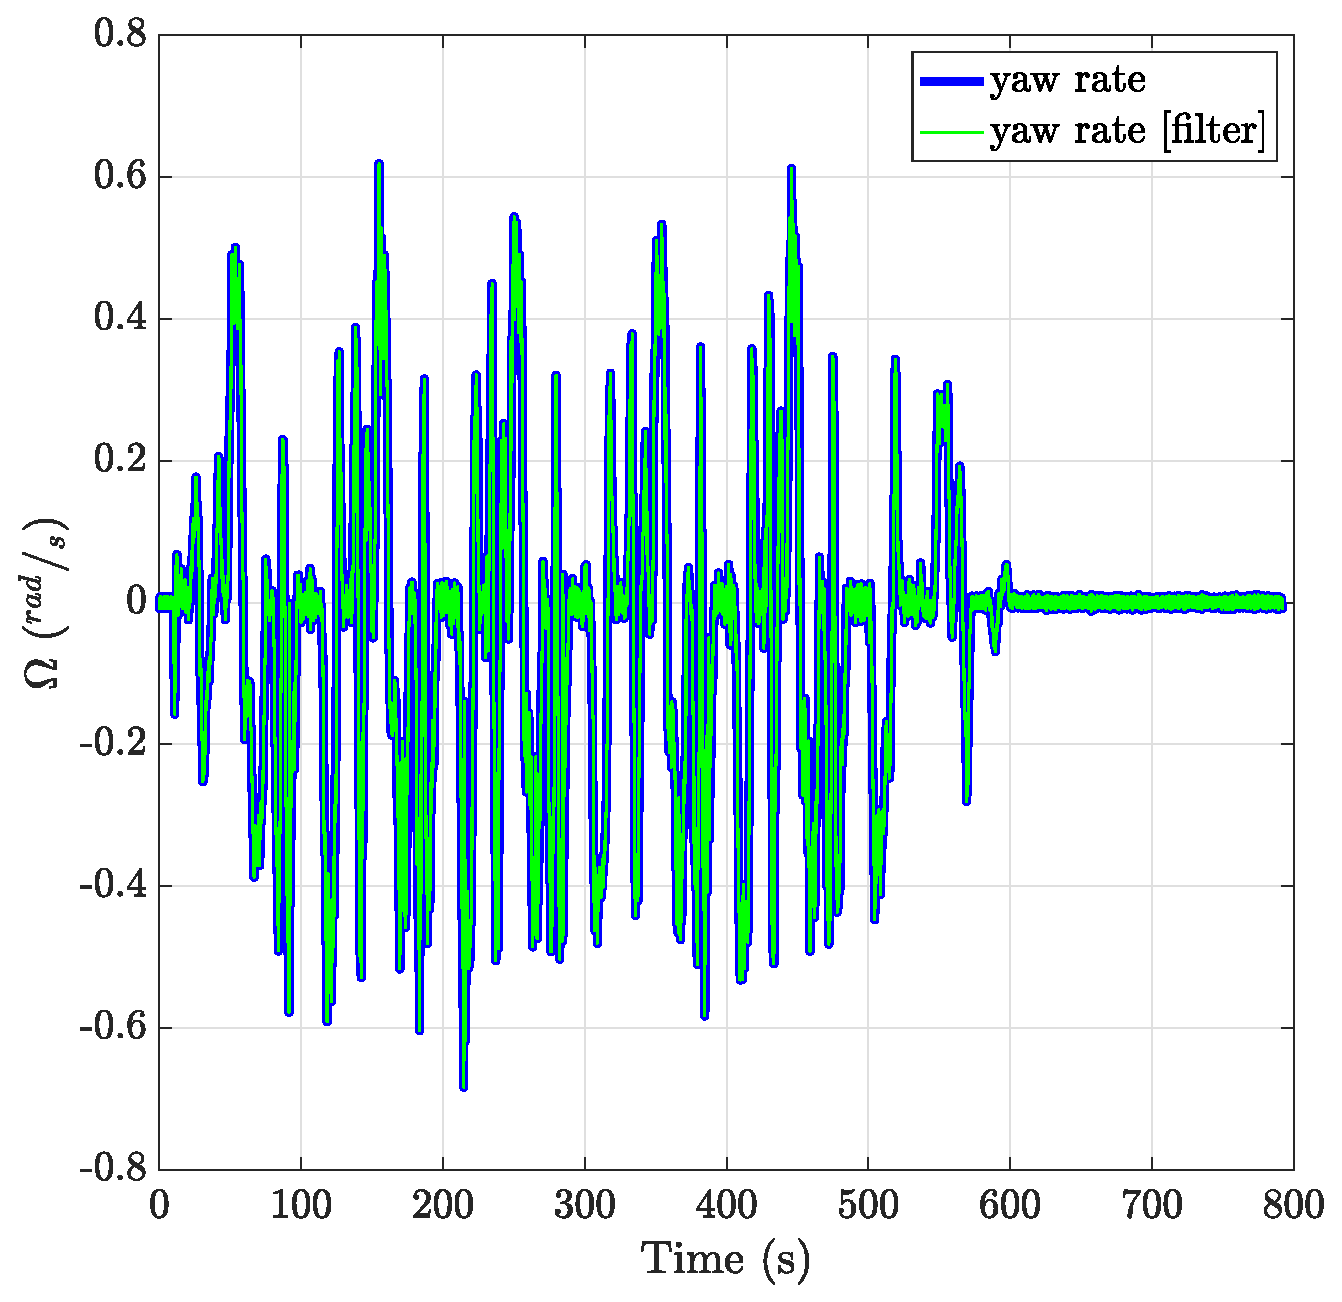
\includegraphics[scale=0.3]{ex3/ex-33.eps}
        \centering
        \caption{filtered INS lateral acceleration vs. the calculated}
        \label{fila}
        \end{figure}

The lateral acceleration was calculated by multiplying the yaw rate by the longitudinal velocity, and is shown in Figure \ref{fila}. 

\textbf{Q. Comparing the longitudinal acceleration measured by INS with the one obtained by derivation of the longitudinal speed measured from the Hall sensors.}

The derived acceleration [shown in Figure \ref{ilavd}] is quite noisier than the one provided by INS. The derived acceleration was filtered using a moving mean. This resulted in a far better matching acceleration compared to the INS data.

        \begin{figure}[ht]
        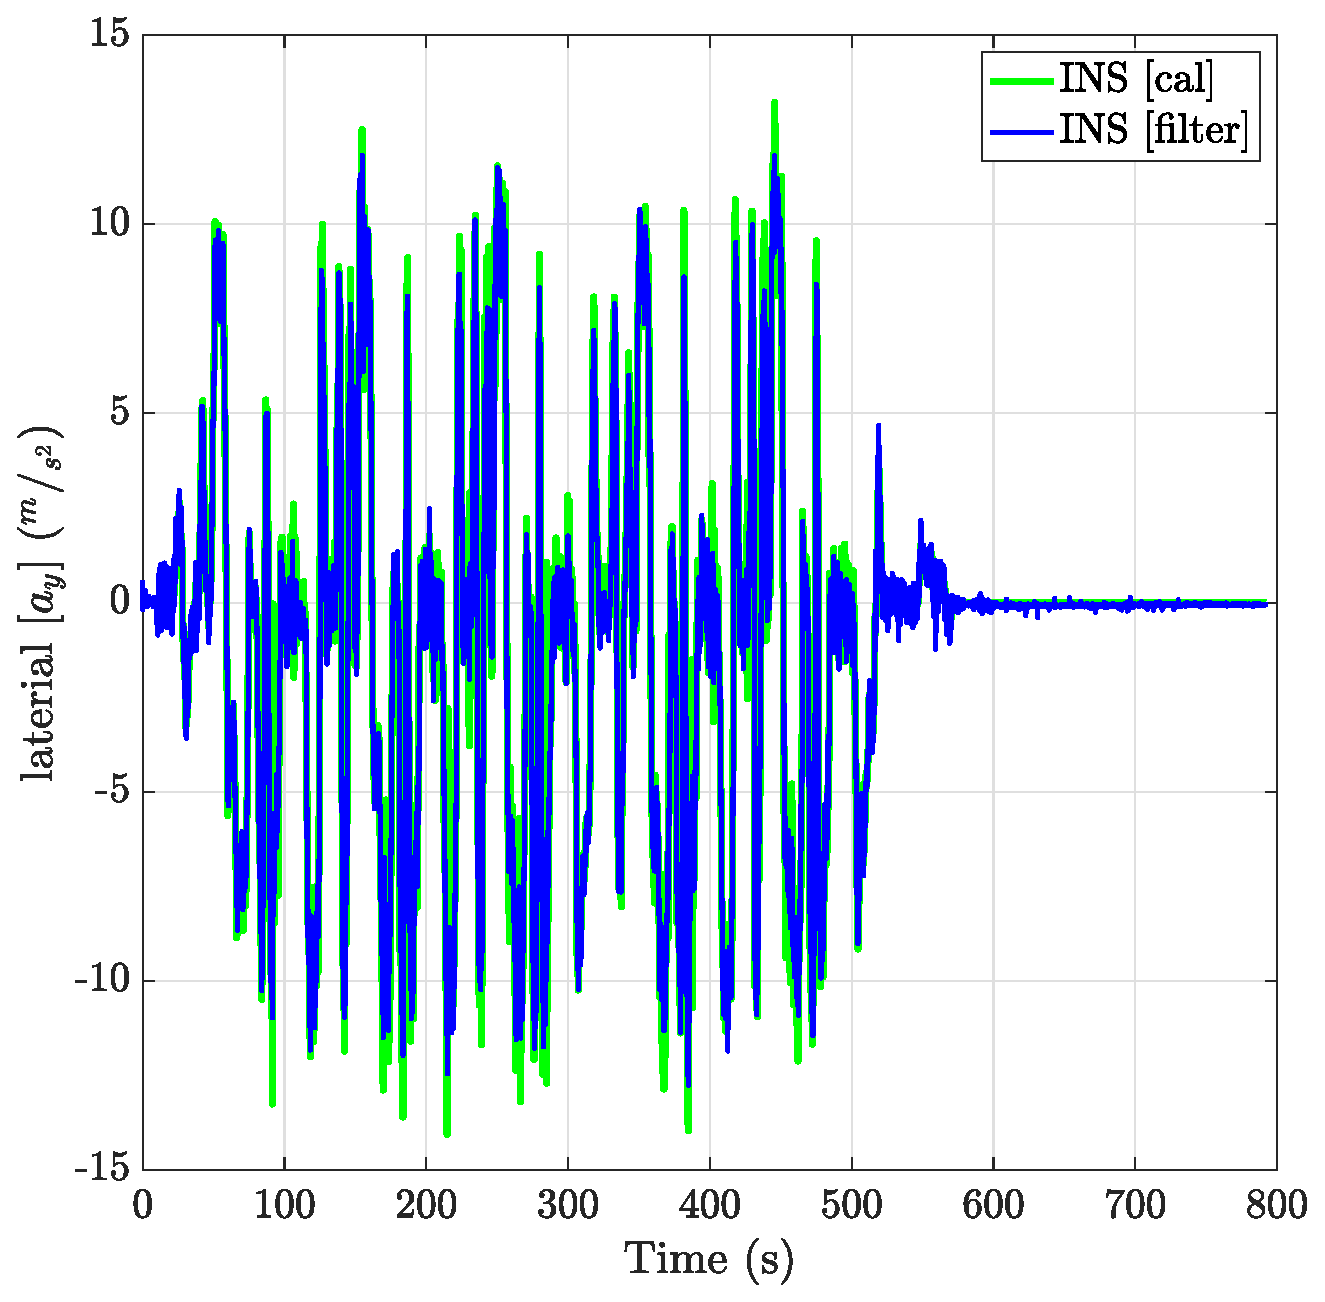
\includegraphics[scale=0.3]{ex3/ex-34.eps}
        \centering
        \caption{The INS longitudinal acceleration vs derived longitudinal acceleration}
        \label{ilavd}
        \end{figure}

\newpage
\textbf{Q. Evaluate the side slip angle.}

In Figure \ref{iavtc}, the side slip angle was calculated using the longitudinal and lateral speed. derived acceleration is quite a lot noisier than the one provided by the INS.

        \begin{figure}[ht]
        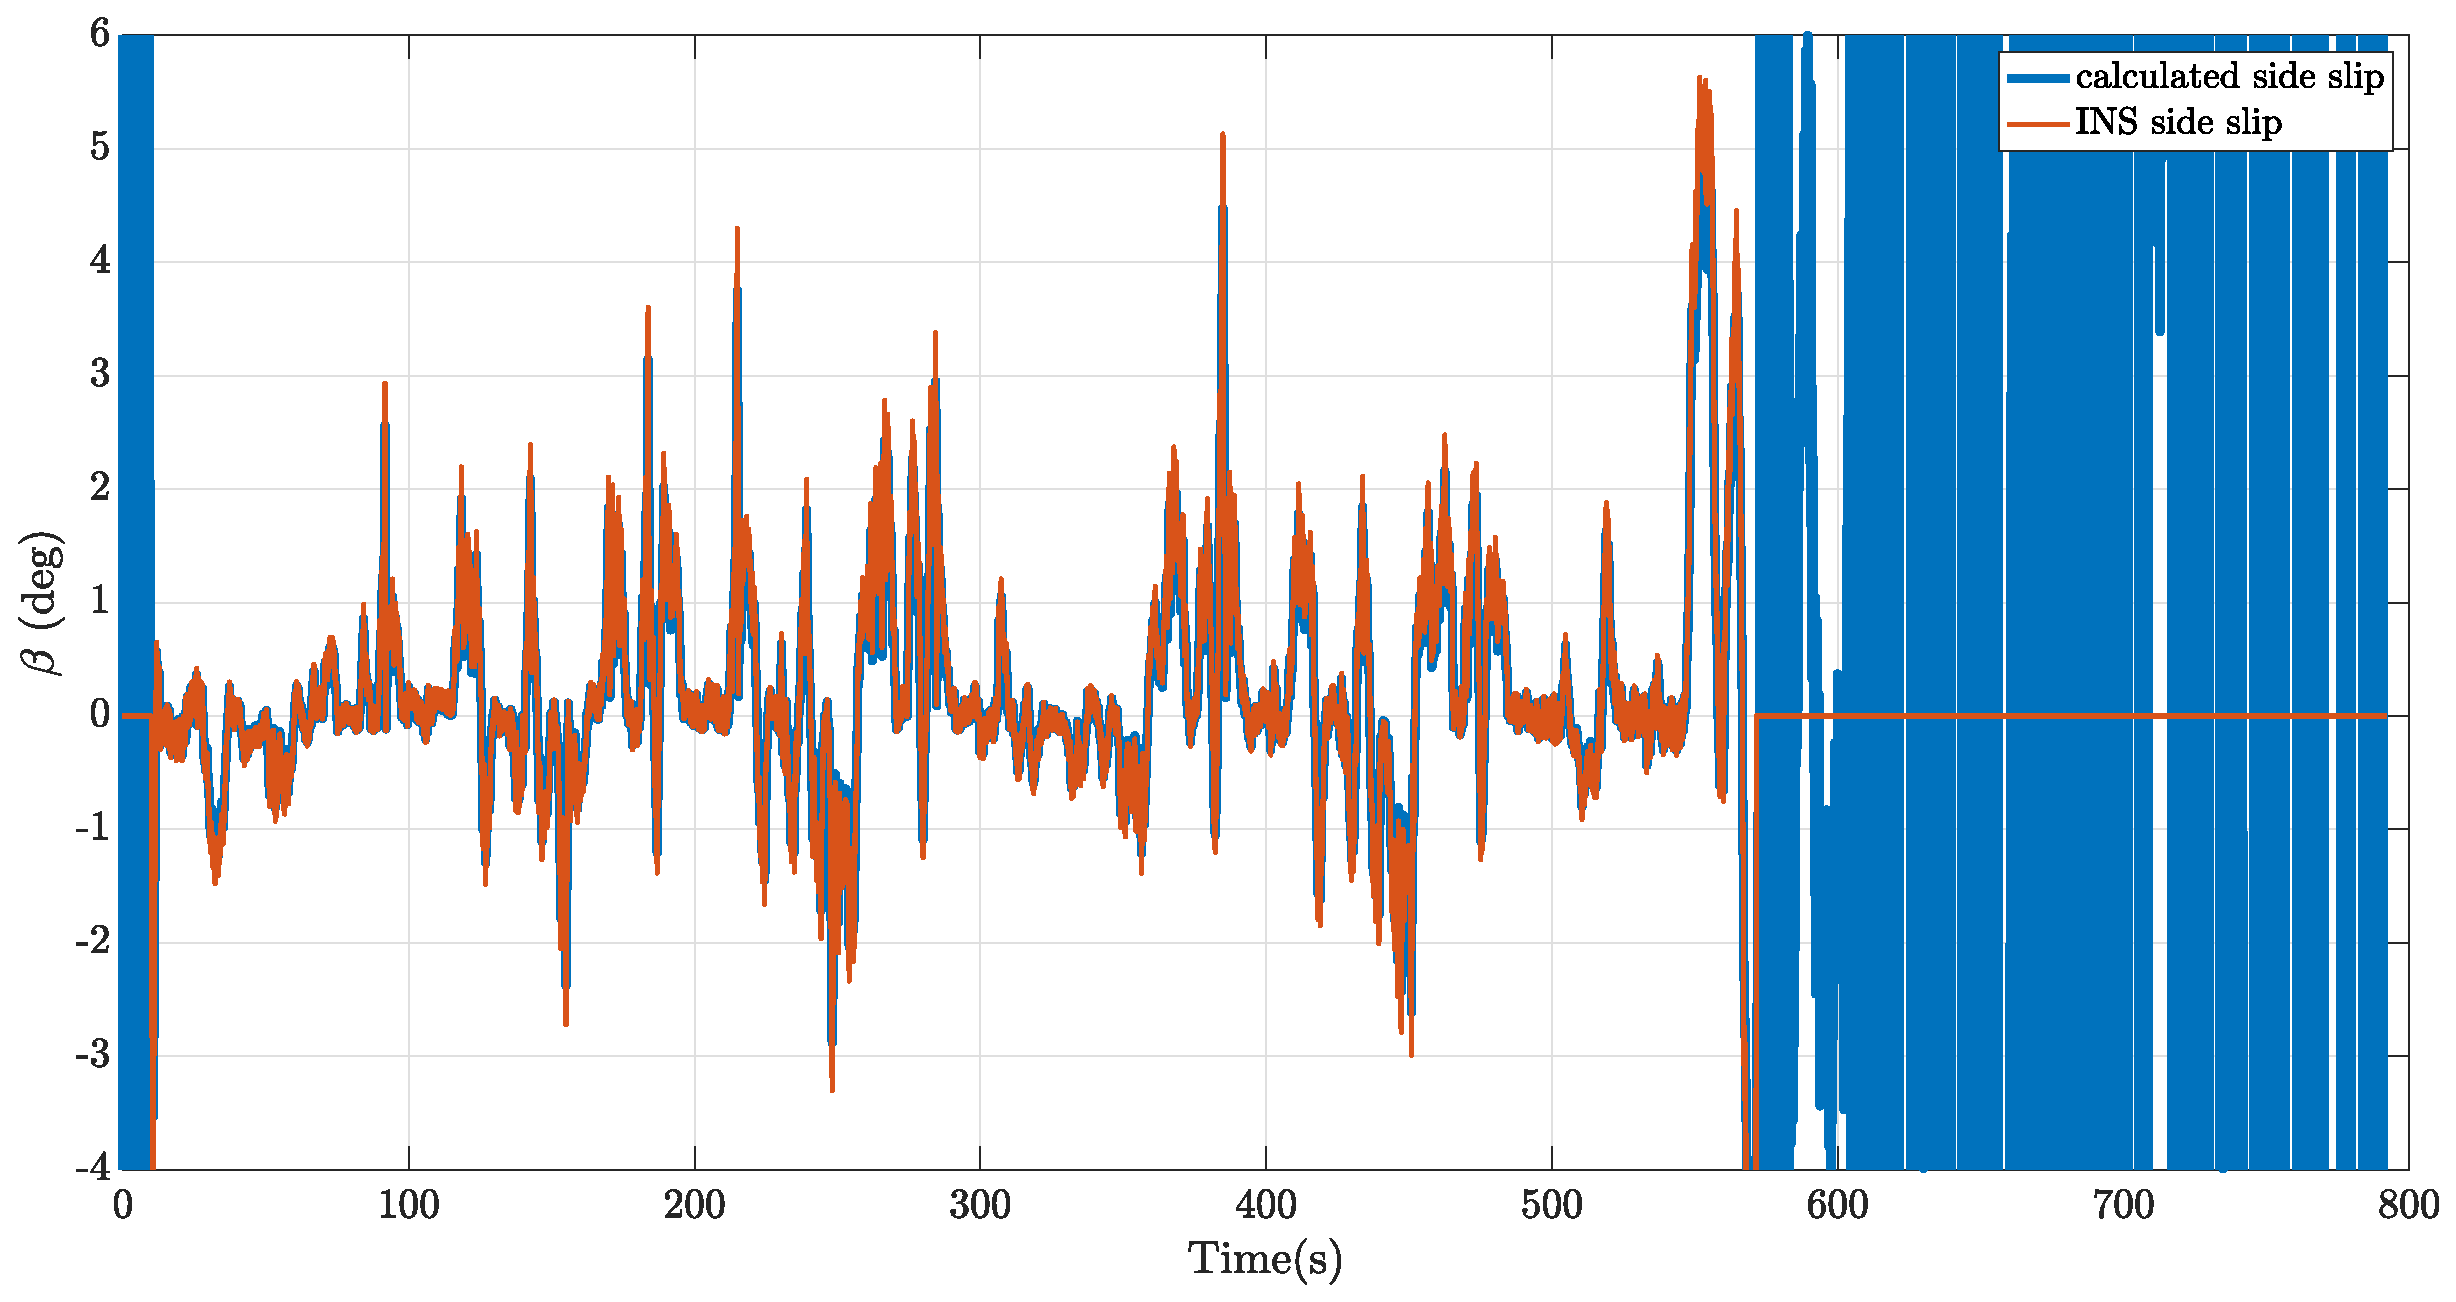
\includegraphics[scale=0.3]{ex3/ex-35.eps}
        \centering
        \caption{the INS angle vs the calculated side slip angle }
        \label{iavtc}
        \end{figure}
\end{document}
\chapter{Vehicle Model Exercises}

\section{Exercise 1 - Vehicle Model Implementation}

\textbf{Q. For each maneuver, plot and comment the main results that you obtain, particularly focusing on tire forces and moments (\{$\fx$, $\fy$, $\fz$, $\mz$\}) and tire slips (\{$\kappa$, $\alpha$\}).}

\begin{enumerate}
  \item initial conditions: $\uz$ = 30 km/h \\
simulation timing: $\ts$\ = 0.001 s, $\tf$\ = 20 s \\
requested pedal: req\_pedal = 1 \\
requested steering wheel angle: req\_steer = 0 deg.
  \end{enumerate}
  
        \begin{figure}[ht]
        
\includegraphics[width=0.99\linewidth]{ex4/q1/ex-41b.eps}
        \centering
        \caption{vehicle motion graphs [maneuver \#1]}
        \label{41b}
        \end{figure}

Figure \ref{41b} shows the motion graphs of the first maneuver. The vehicle starts from 30 km/h, with no steering input and full throttle. The velocity increased until it reached full speed of 108 km/h within 5 seconds. All upcoming graphs are influenced by the acceleration profile.

        \begin{figure}[ht]
        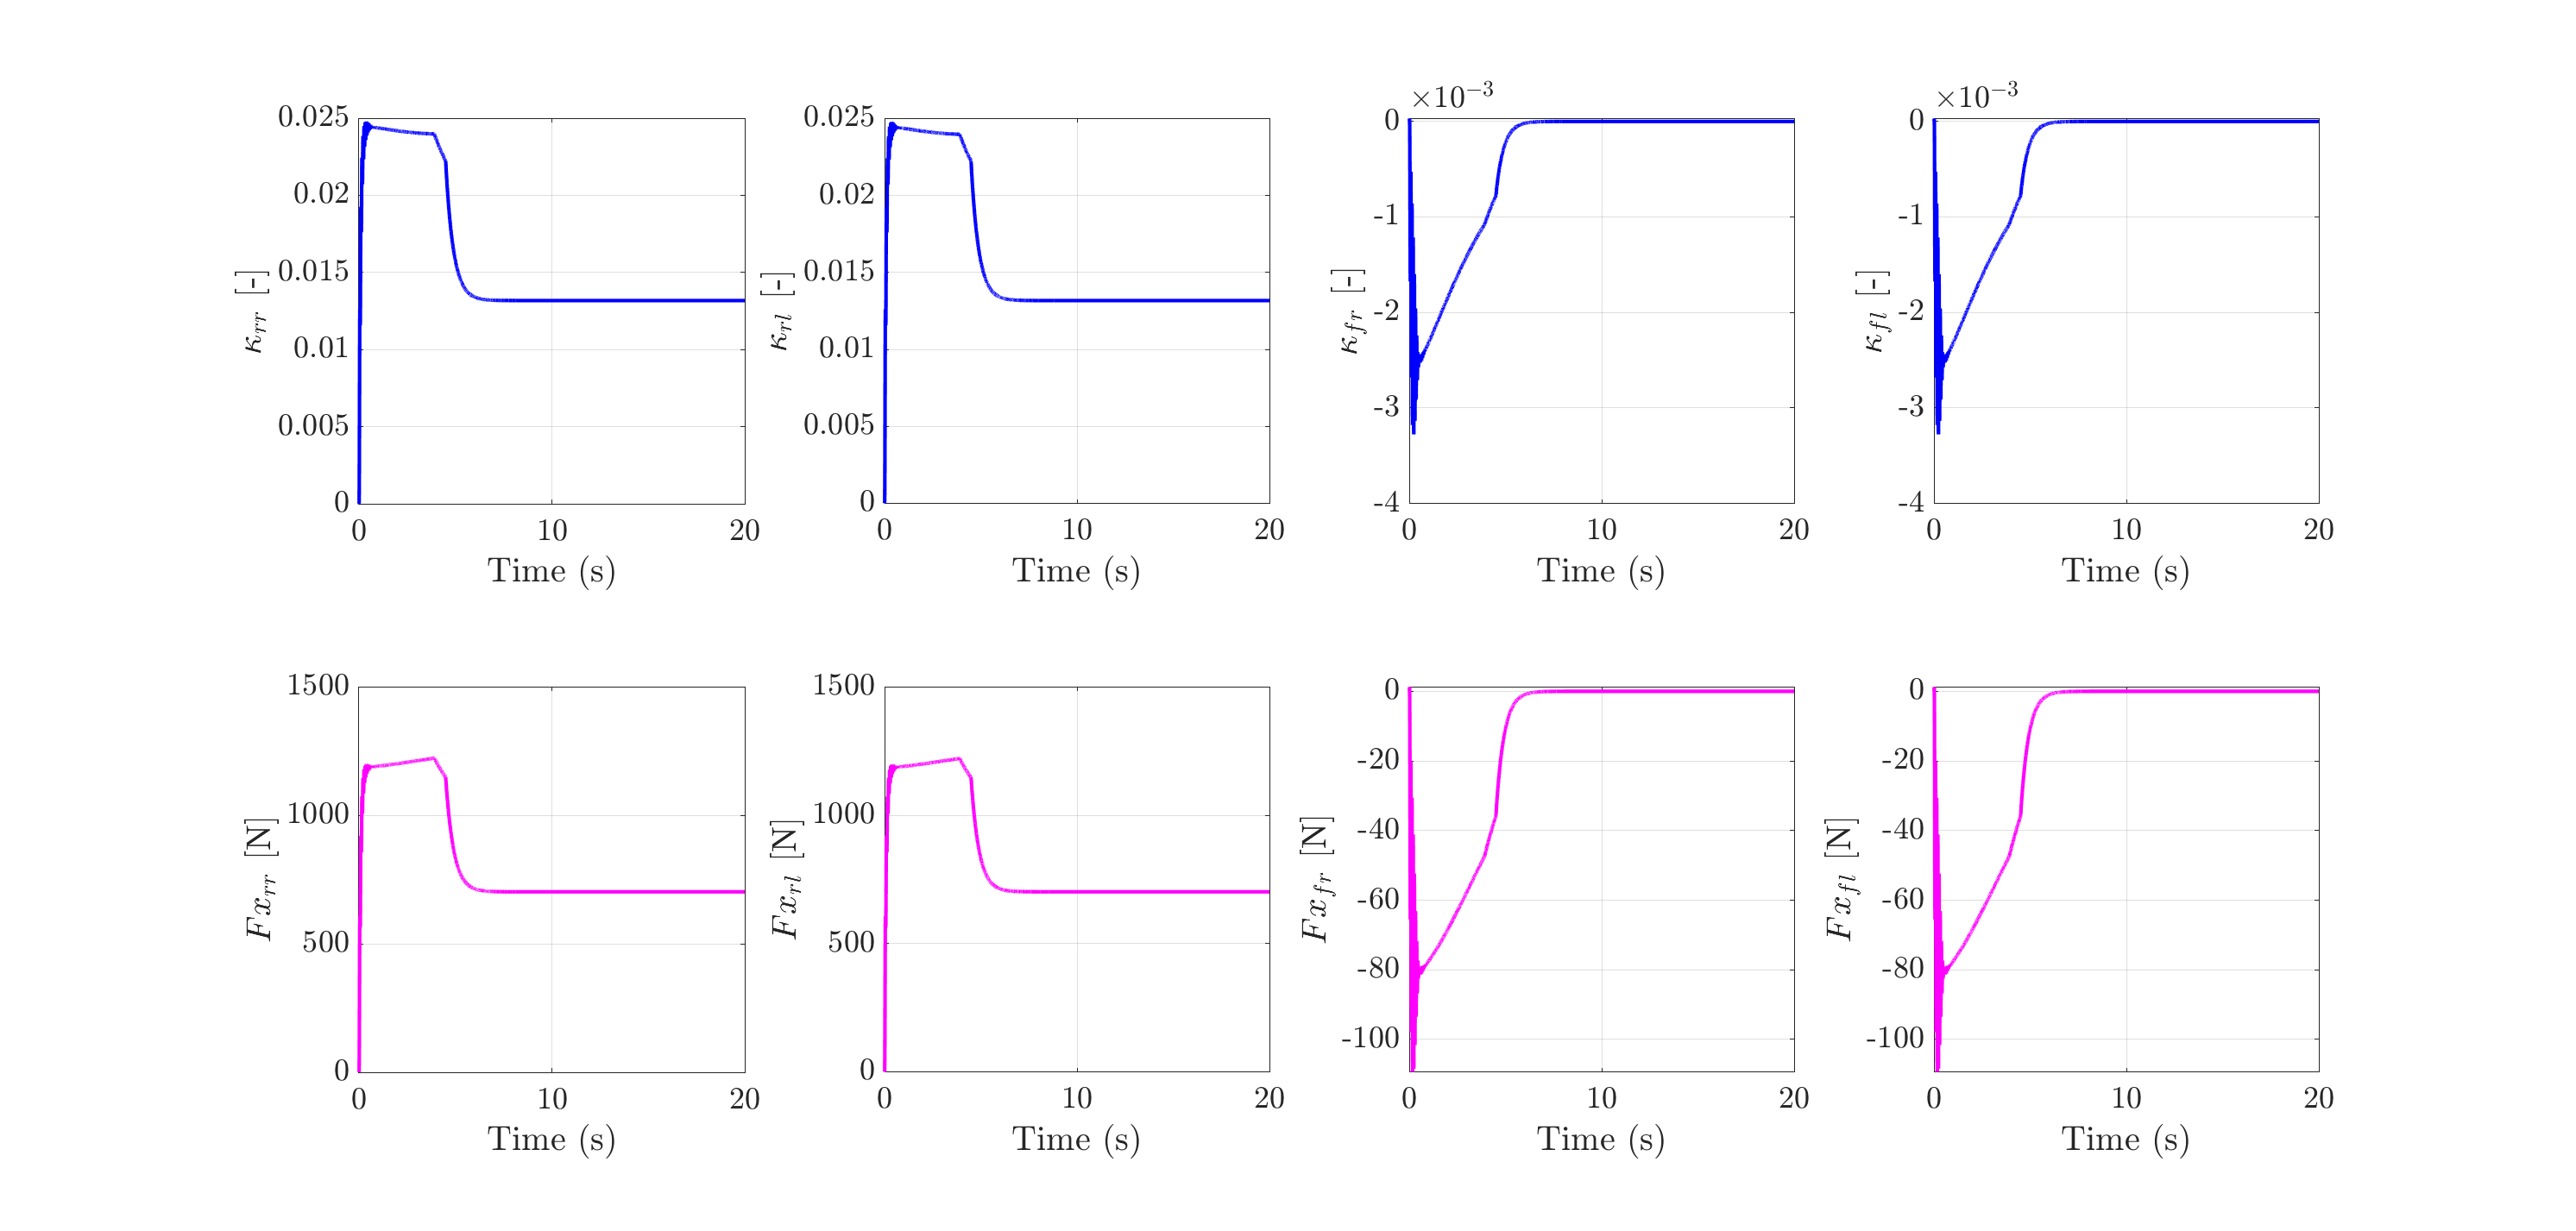
\includegraphics[width=0.85\linewidth]{ex4/q1/ex-41f.eps}
        \centering
        \caption{longitudinal slip $\kappa$ and longitudinal forces $\fx$ [maneuver \#1]}
        \label{41f}
        \end{figure}
        
The graphs in Figure \ref{41f} shows no difference between both right tires [and similarly the left tires] as the vehicle was moving straight without steering input. However, both rear tires show much higher $\kappa$ and $\fy$. This was expected as the vehicle is rear-wheel drive and torque applied from the motors would increase both the slip and force experienced by the rear tires.

During the vehicle's acceleration to maximum speed [between 0 and 5 seconds] all tires showed higher slip and force. Once maximum speed is reached [acceleration is zero], the slips and forces decrease across all tires. The front tires go to zero, while the rears do not, as the motors must still keep applying [decreased] torque to keep the vehicle at speed.

        \begin{figure}[ht]
        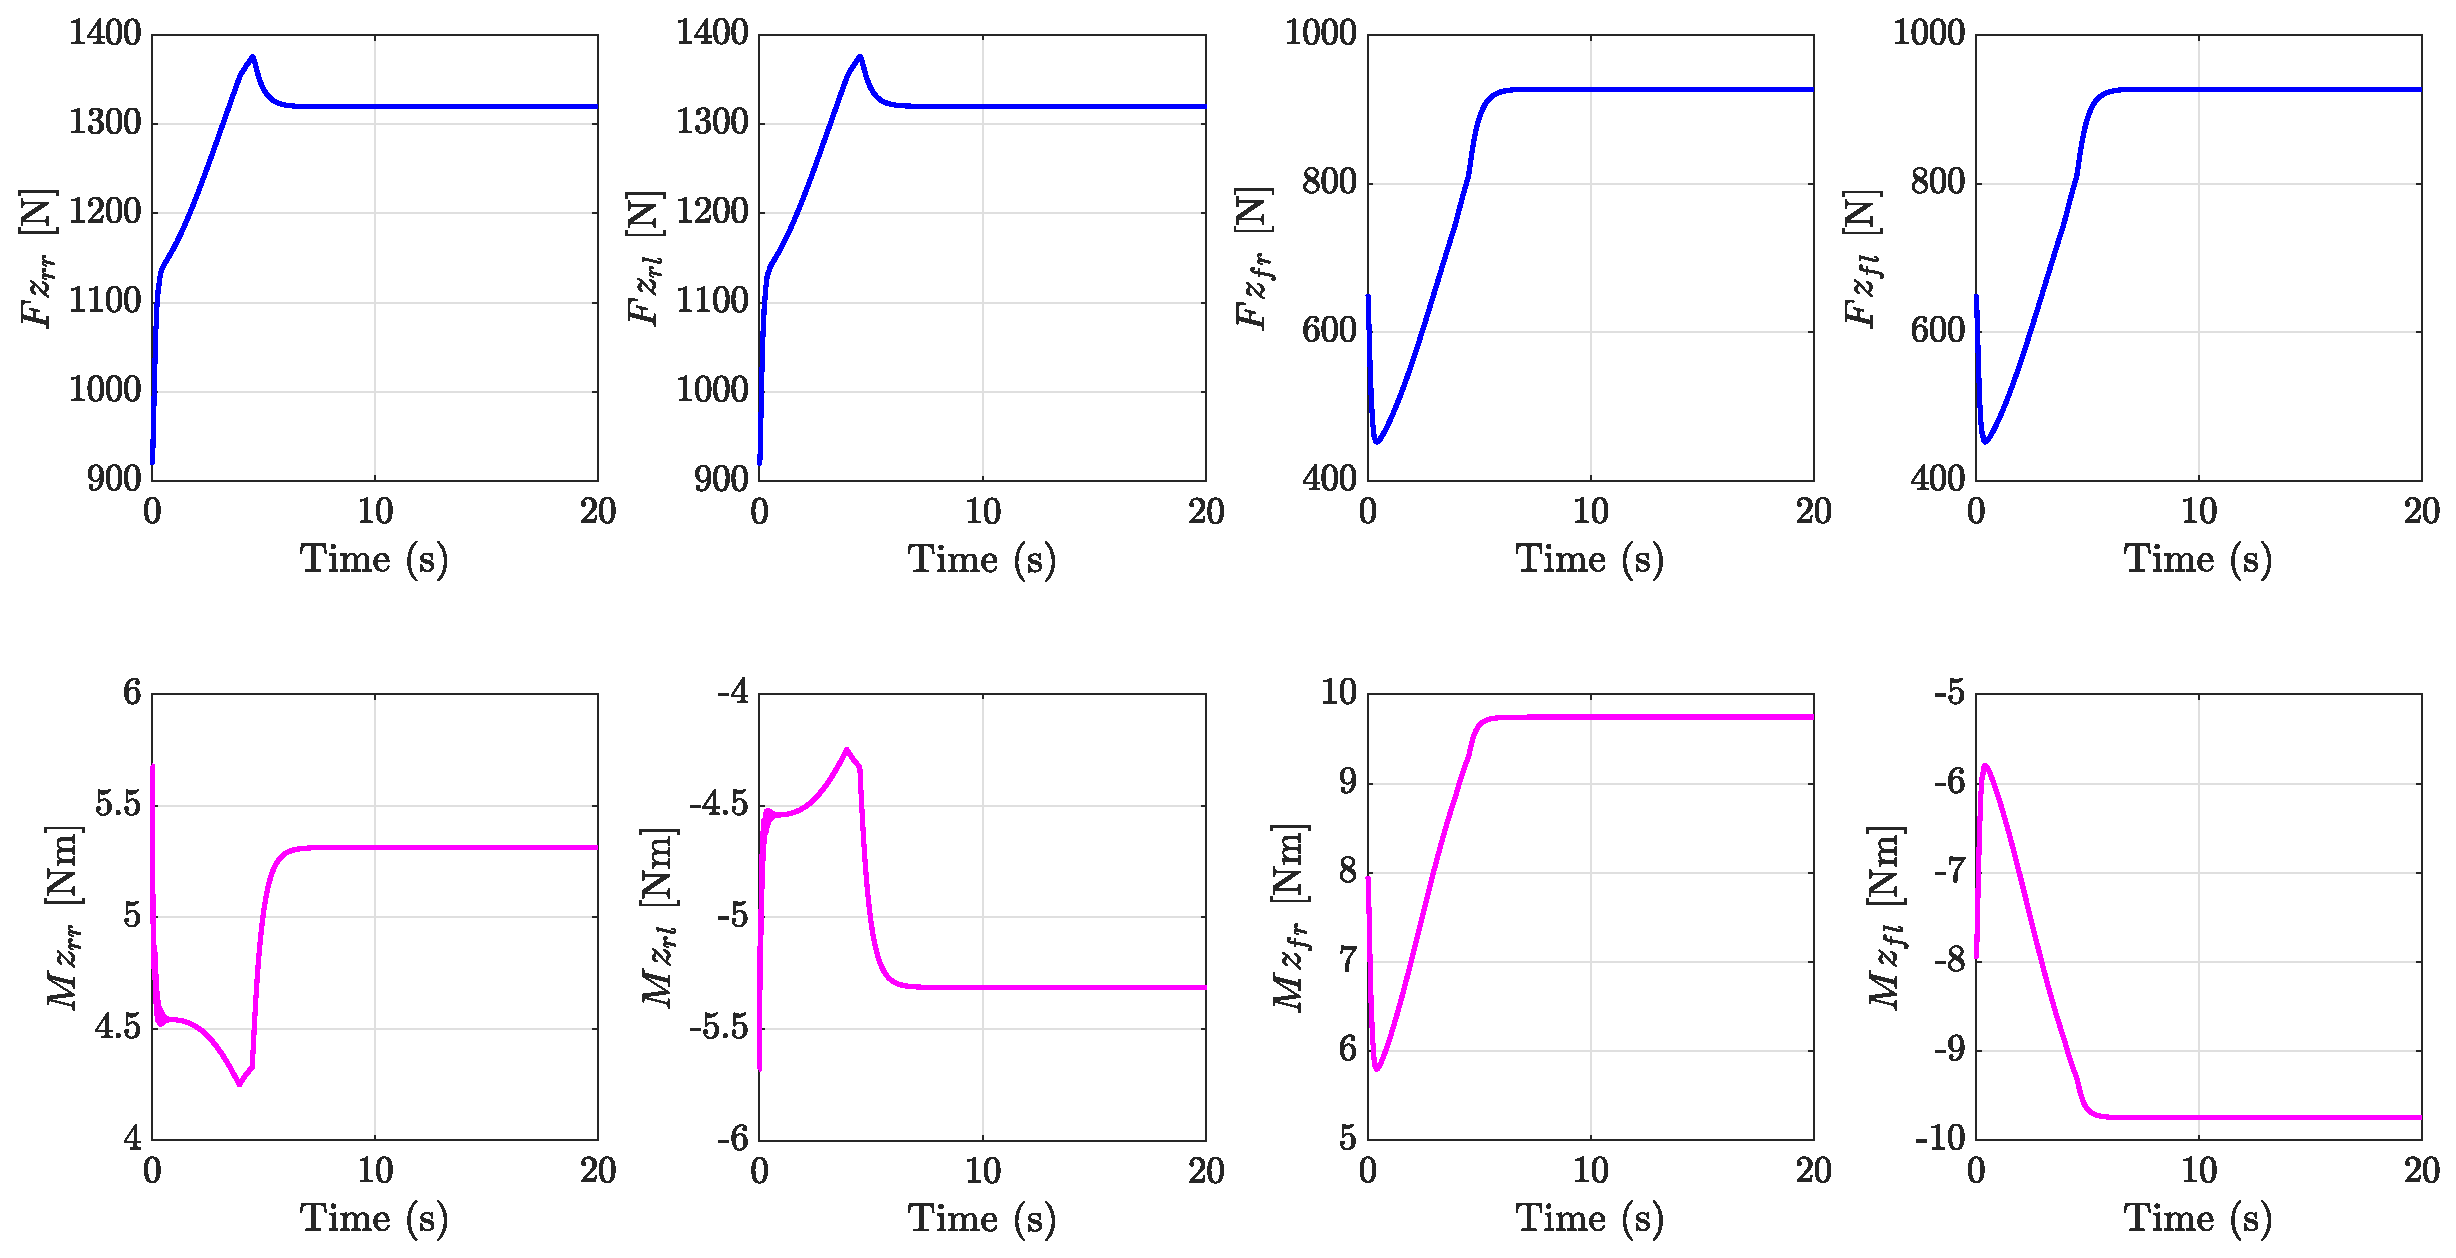
\includegraphics[width=0.85\linewidth]{ex4/q1/ex-41h.eps}
        \centering
        \caption{Vertical forces $\fz$\ and self aligning torque $M_{z}$ [maneuver \#1]}
        \label{41h}
        \end{figure}
        
The aerodynamics load $\fa$\ increases as speed increases. As shown in Figure \ref{41h}, the vertical force $\fz$ increases across all tires because it relies on $\fa$. The vertical loads are calculated using Equation \ref{eq:4.1}:

\begin{equation}\label{eq:4.1}
\begin{aligned}
    \fzr = mg \frac{\lf}{L} + \fazr + \fx \frac{\hg}{L} - \frac{\iyz}{L} \dot{\Omega} \\
    \fzf = mg \frac{\lr}{L} + \fazf + \fx \frac{\hg}{L} - \frac{\iyz}{L} \dot{\Omega}
\end{aligned}
\end{equation}

They later reach steady state once the car stops accelerating. the rear tires show a peak in $\fz$ due to the drop in acceleration $\ay$ towards nearing maximum speed, which decreased the lateral load transfer on the rear tires.
        
        \begin{figure}[ht]
        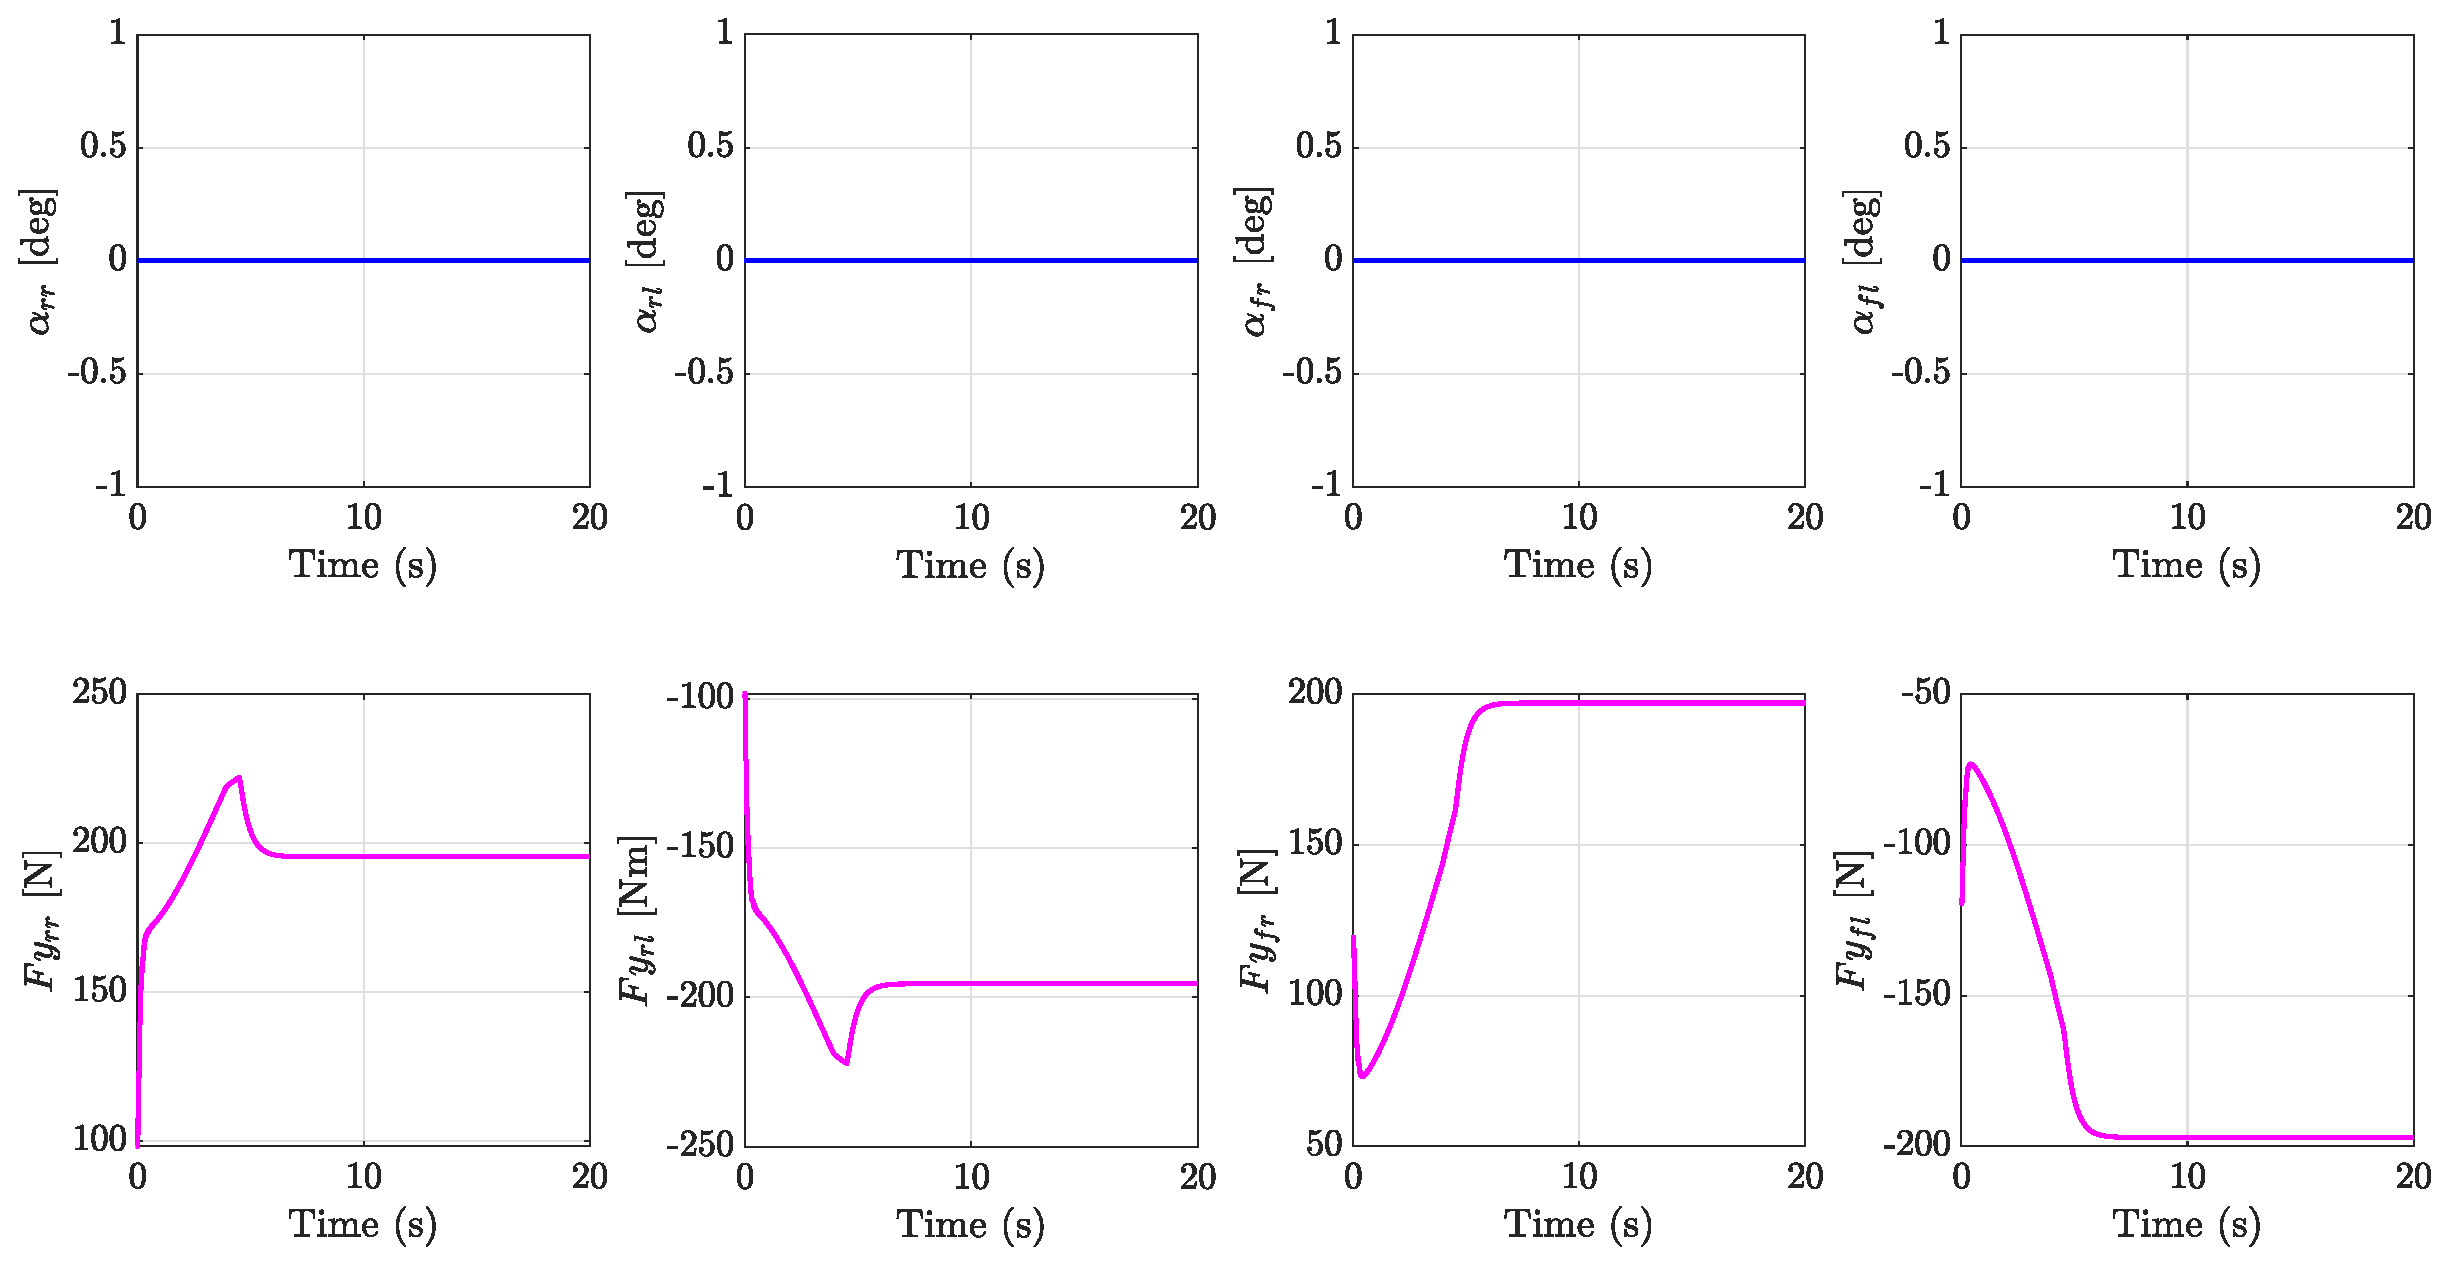
\includegraphics[width=0.85\linewidth]{ex4/q1/ex-41d.eps}
        \centering
        \caption{side slip angle $\alpha$ and lateral forces $\fy$ [maneuver \#1]}
        \label{41d}
        \end{figure}

As previously mentioned, the vehicle has no steering input, which is why the side slip angle $\alpha$ for all tires are zero [Figure \ref{41d}]. Furthermore, the magnitude of the lateral forces on the right tires are equal [and similarly the left tires]. The right tires' lateral forces are opposite in direction compared to the left tires and equal in magnitude, thus making them cancel out keeping the vehicle moving straight. $\fy$\ is smaller than $\fx$\ for all the tires. The self aligning torque $\mz$ profiles previously shown in Figure \ref{41h} resemble the lateral forces profiles for each tire as they are trying to counter their effect on the steering.

During acceleration, the lateral forces $\fy$ across all tires increase because the vertical forces $\fz$ increased. The lateral forces relies on the vertical forces in the pacejka calculations, which is why both the $\fy$ and $\fz$ profiles match for front and rear tires.

% \vspace{-1em}
\newpage
\begin{enumerate}[resume]
  \item initial conditions: $\uz$ = 100 km/h \\
simulation timing: $\ts$\ = 0.001 s, $\tf$\ = 1.5 s \\
requested pedal: req\_pedal = -1 \\
requested steering wheel angle: req\_steer = 0 deg.
  \end{enumerate}

        \begin{figure}[ht]
        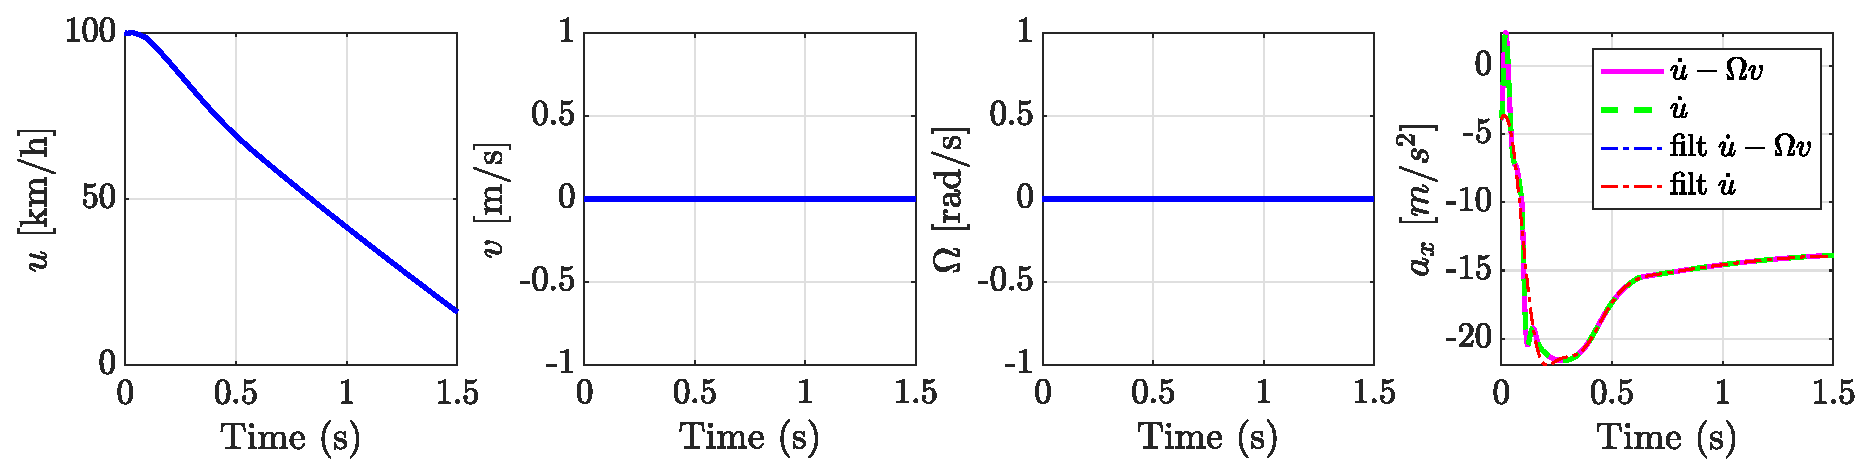
\includegraphics[width=0.99\linewidth]{ex4/q2/ex-42b.eps}
        \centering
        \caption{vehicle motion graphs [maneuver \#2]}
        \label{42b}
        \end{figure}

Figure \ref{42b} shows the motion graphs of the second maneuver. The vehicle starts from 100 km/h, with no steering input and applying full brakes. The velocity dropped to 16 km/h within the specified 1.5 seconds. The deceleration shows a decrease after 0.27 seconds as the rear tires start slipping and going into a full wheel lock as shown in Figure \ref{42f}.

        \begin{figure}[ht]
        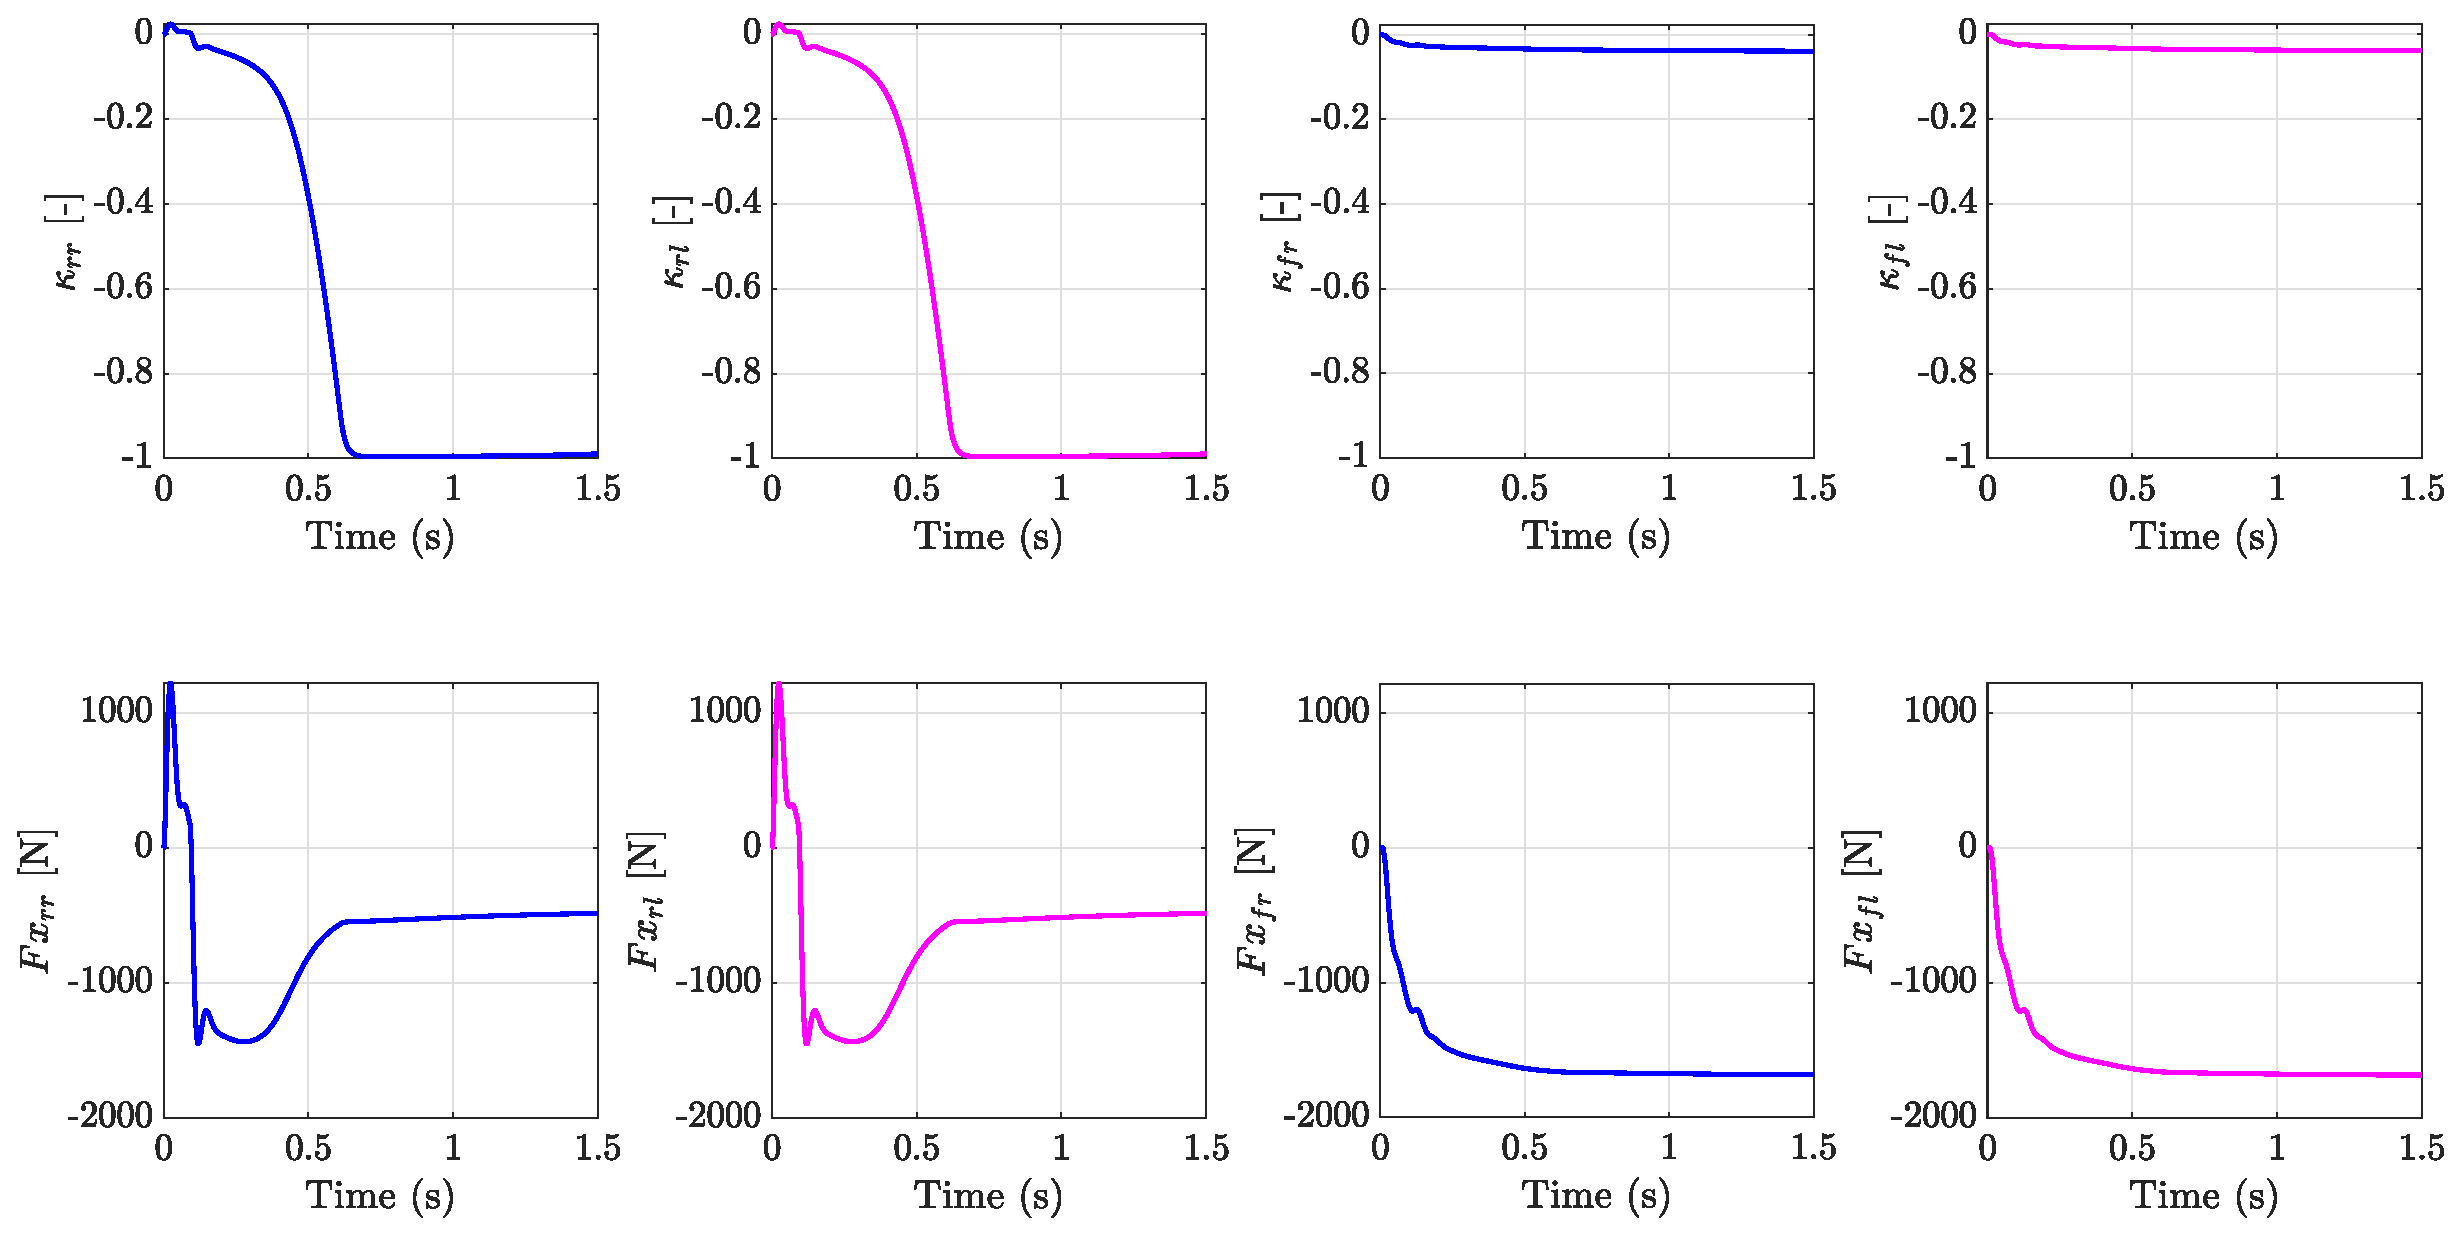
\includegraphics[width=0.85\linewidth]{ex4/q2/ex-42f.eps}
        \centering
        \caption{longitudinal slip $\kappa$ and longitudinal forces $\fx$ [maneuver \#2]}
        \label{42f}
        \end{figure}
        
This maneuver also doesn't have steering input, which is why the graphs in Figure \ref{42f} show no difference between both right and left tires. The longitudinal forces $\fx$ for all tires increase in the opposite direction because the vehicle is decelerating. The longitudinal slip $\kappa$ for the rear tires go to -1, which means both tires went into wheel lock. $\fx$ decreases once wheel lock starts to occur causing lower efficiency in braking and the deceleration rate decreases.

        \begin{figure}[ht]
        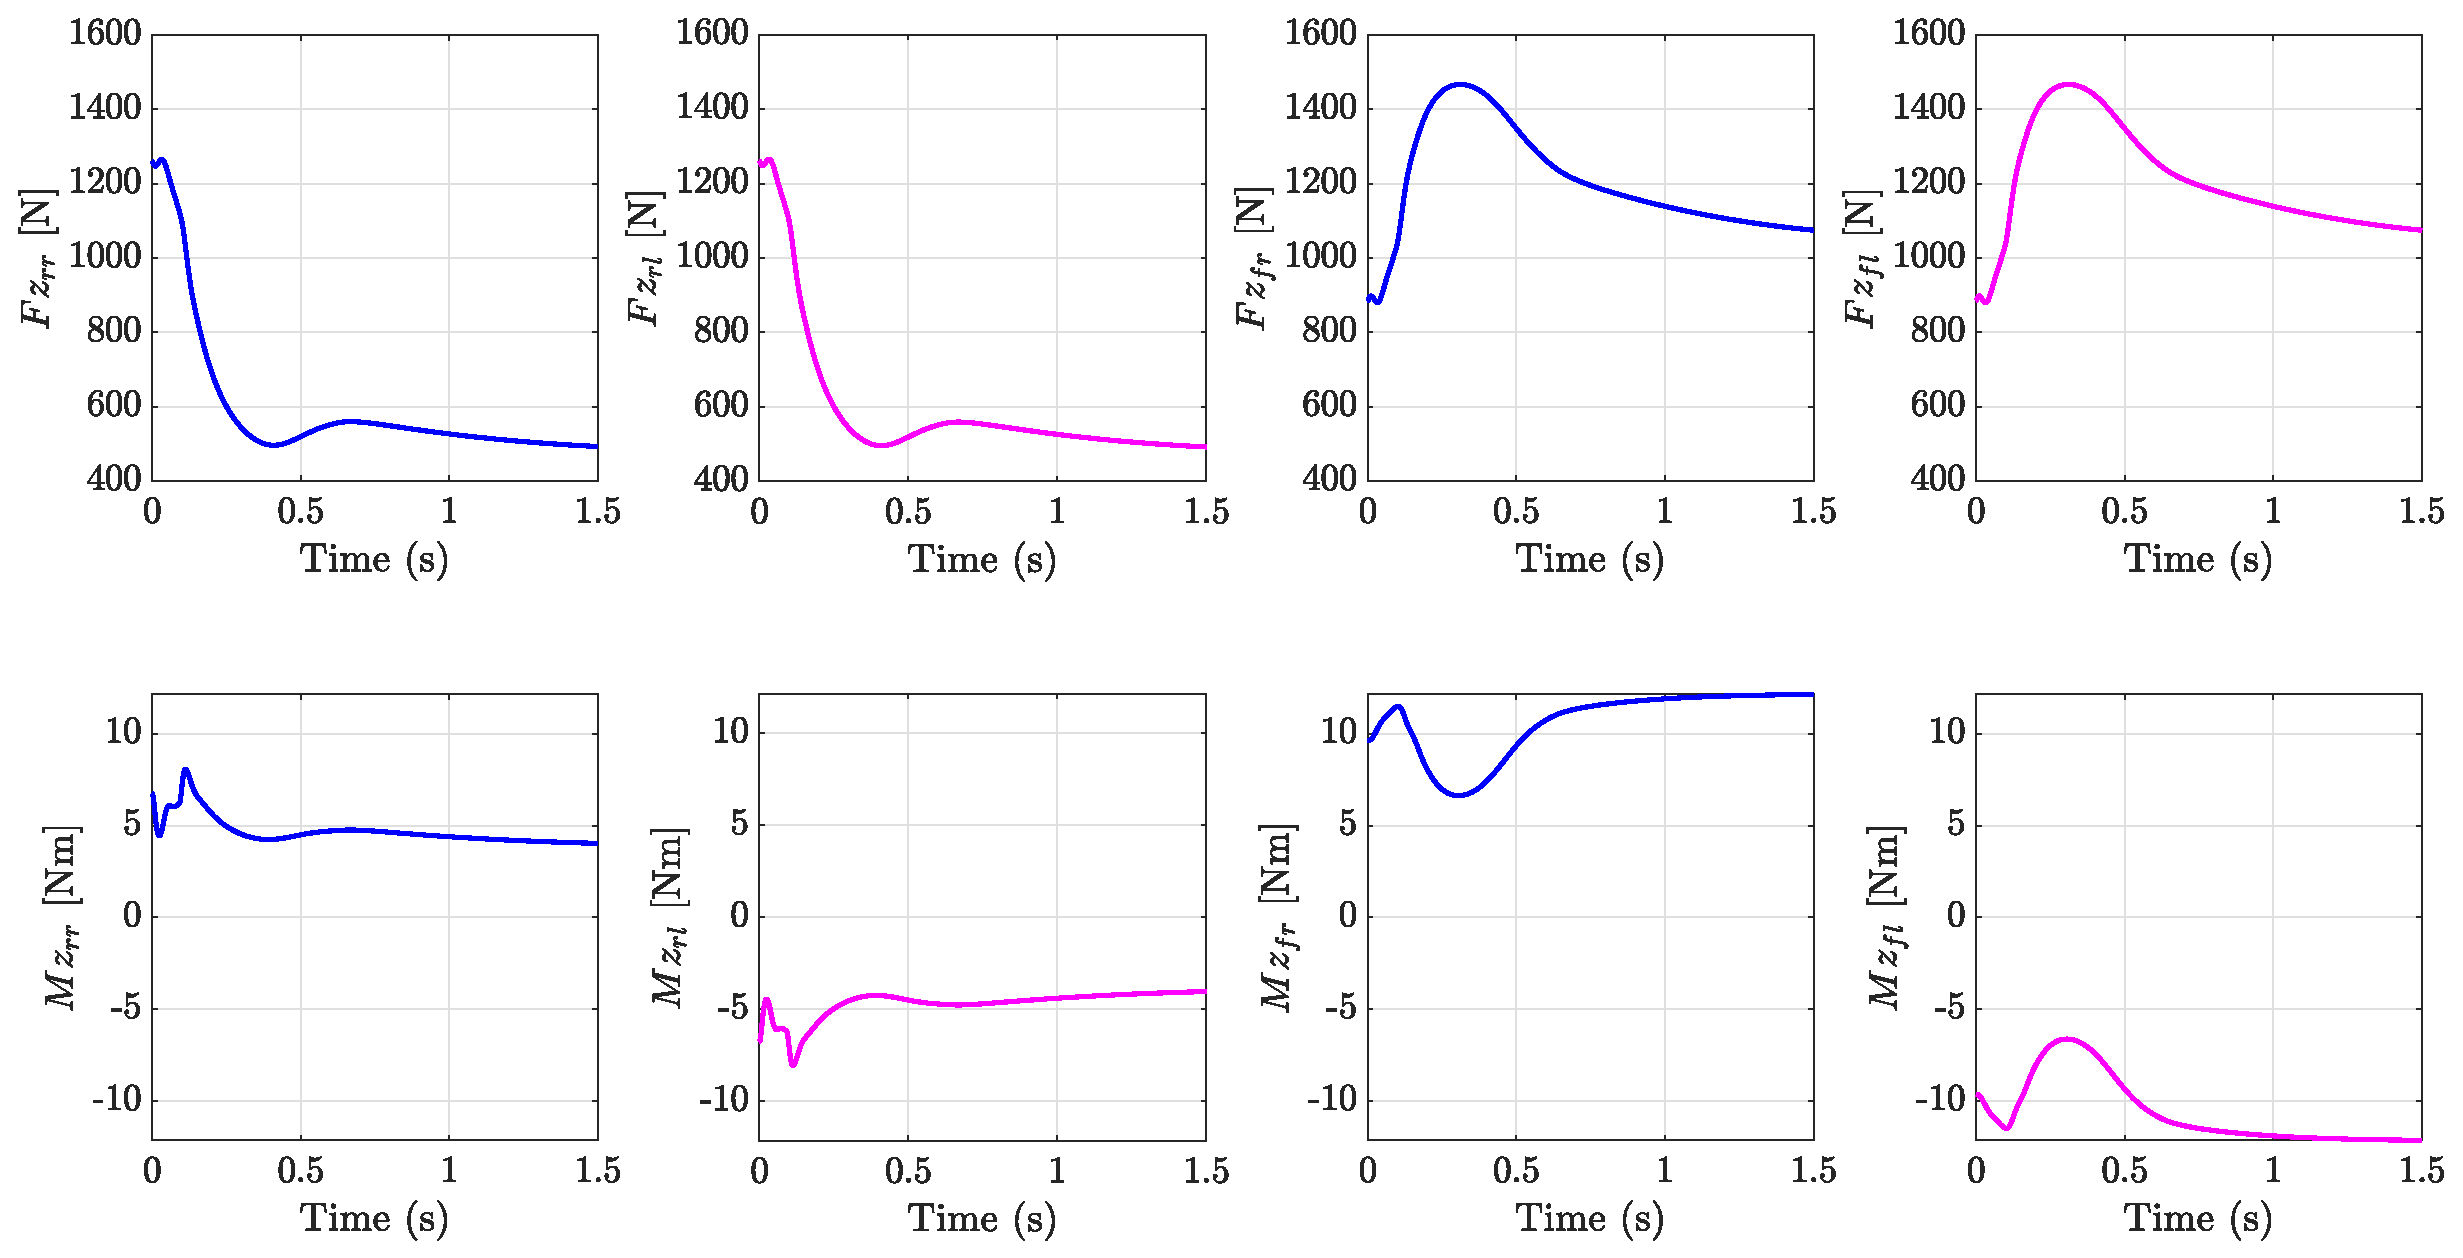
\includegraphics[width=0.85\linewidth]{ex4/q2/ex-42h.eps}
        \centering
        \caption{Vertical forces $\fz$\ and self aligning torque $M_{z}$ [maneuver \#2]}
        \label{42h}
        \end{figure}

Figure \ref{42h} shows the vertical force $\fz$ has decreased in the rear tires while increasing in the front. This is attributed to the longitudinal load transfer to the front because of the braking. The $\fz$ forces on all tires showed a peak around 0.27 seconds due to the rear wheels locking.

No steering input means no side slip angle $\alpha$ for all tires [Figure \ref{42d}]. And similar to maneuver \#1, the right tires' lateral forces are opposite in direction compared to the left tires and equal in magnitude. The self aligning torque $\mz$ profiles in Figure \ref{42h} for each tire are trying to counter the $\fy$'s effect on the steering. $\fy$ showed the same trend as $\fz$, increasing in the front while decreasing in the rear tires.

        \begin{figure}[ht]
        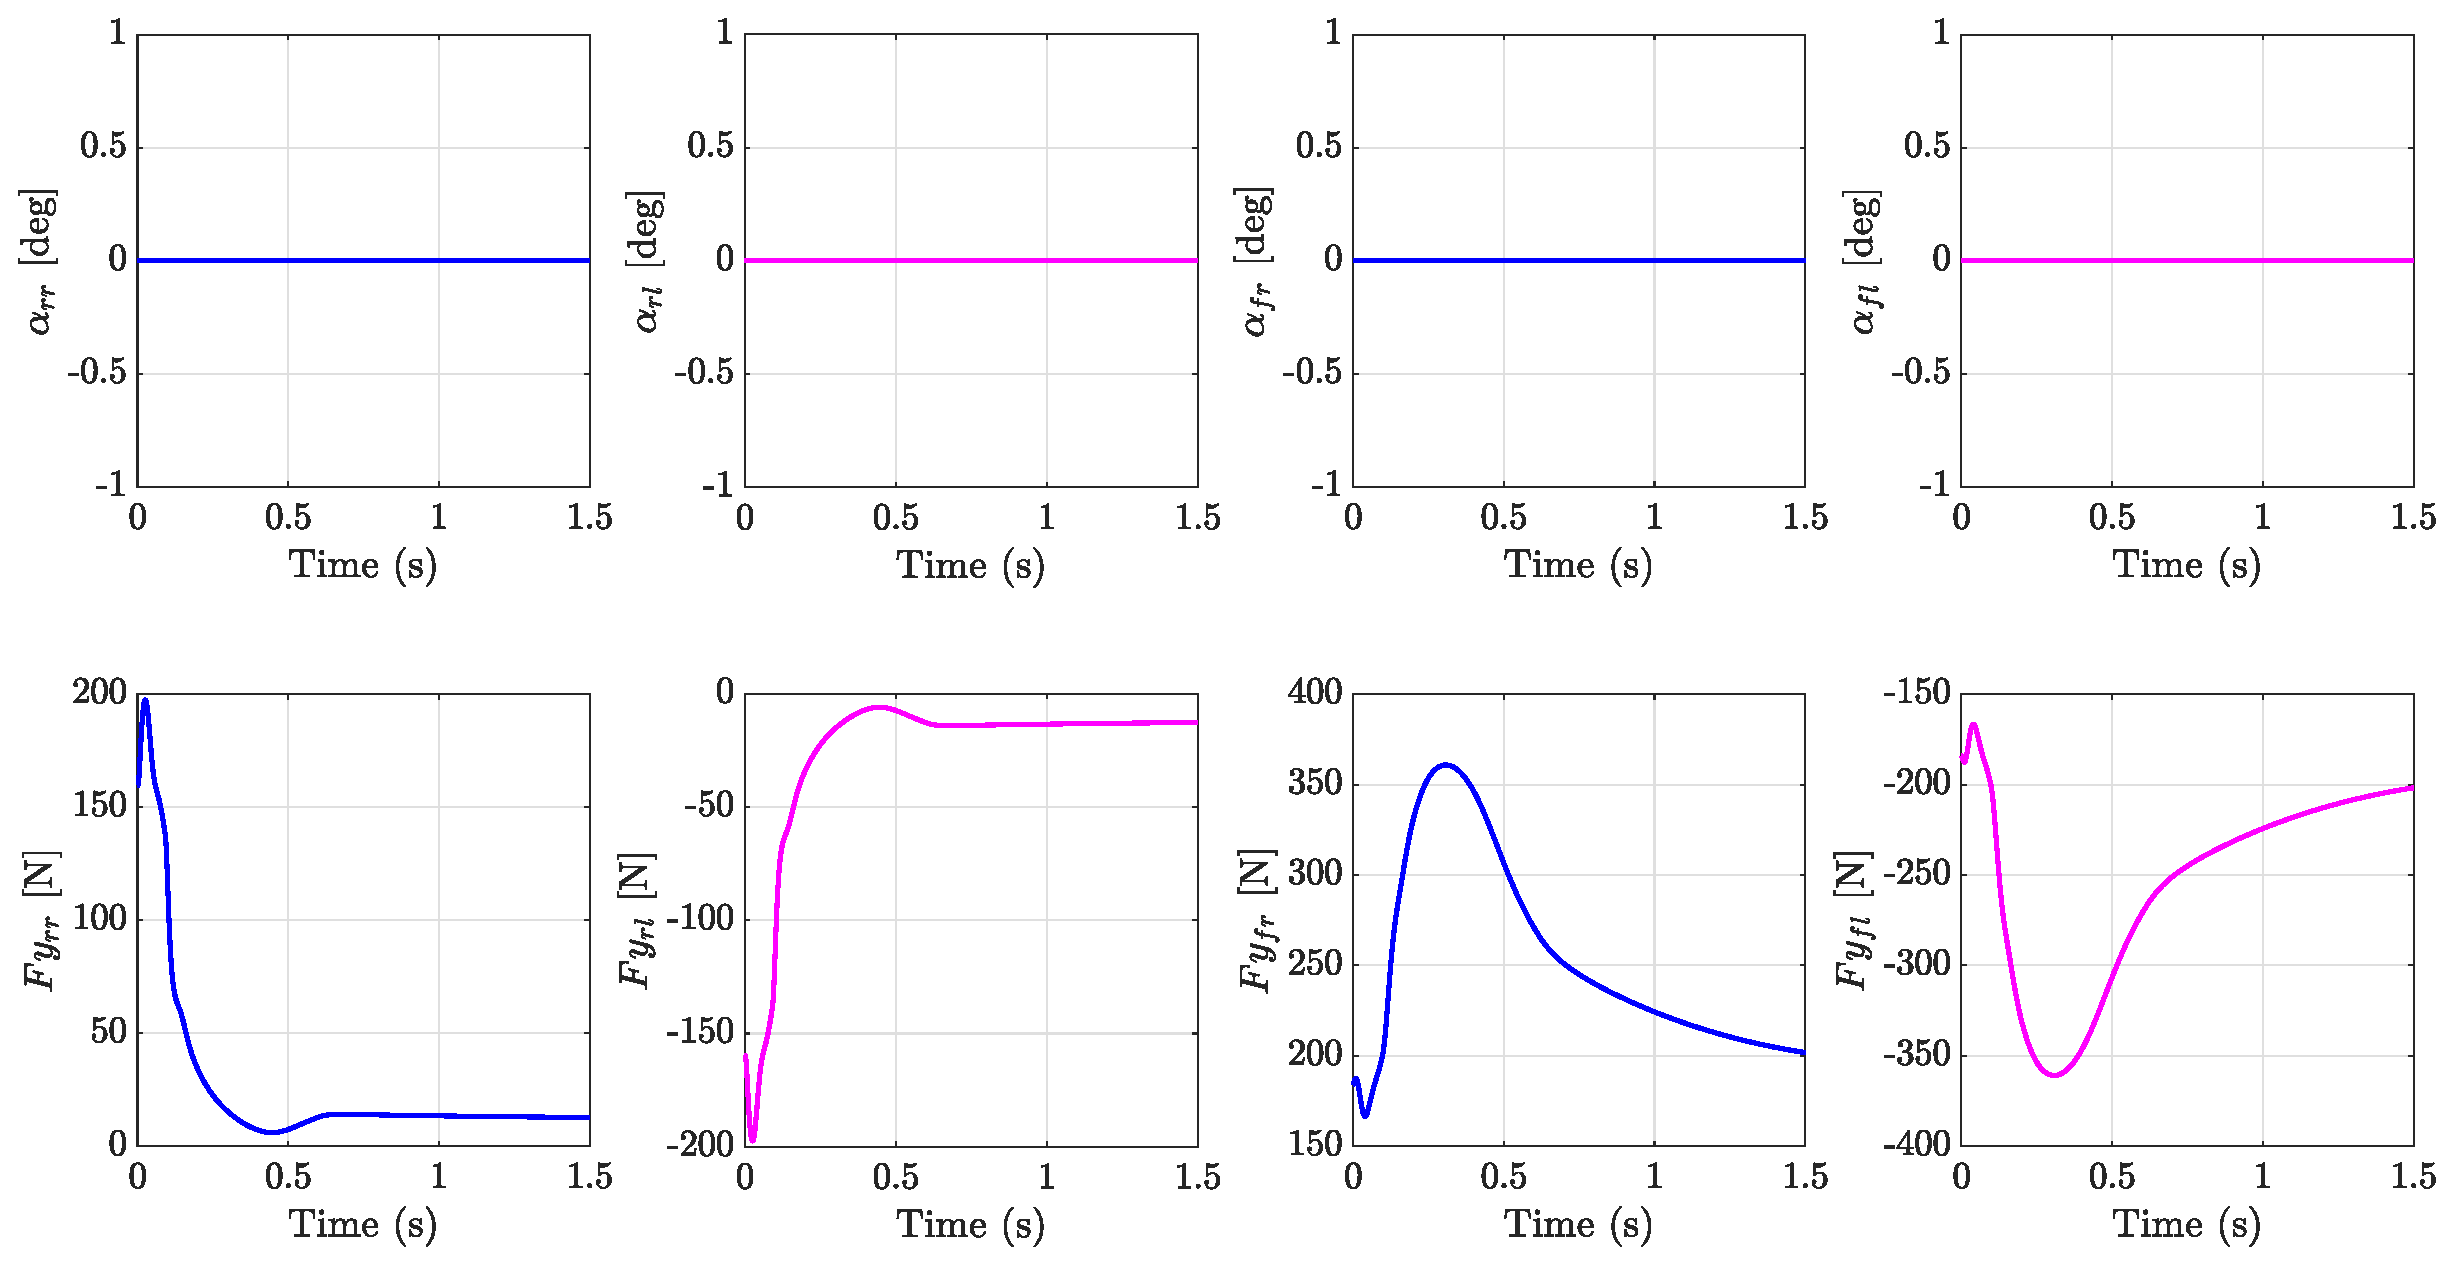
\includegraphics[width=0.85\linewidth]{ex4/q2/ex-42d.eps}
        \centering
        \caption{side slip angle $\alpha$ and lateral forces $\fy$ [maneuver \#2]}
        \label{42d}
        \end{figure}
\newpage
\begin{enumerate}[resume]
  \item initial conditions: $\uz$ = 50 km/h \\
simulation timing: $\ts$\ = 0.001 s, $\tf$\ = 1.5 s \\
requested pedal: req\_pedal = 0.5 \\
requested steering wheel angle: req\_steer = 20 deg.
  \end{enumerate}


        \begin{figure}[ht]
        
\includegraphics[width=0.99\linewidth]{ex4/q3/ex-43b.eps}
        \centering
        \caption{vehicle motion graphs [maneuver \#3]}
        \label{43b}
        \end{figure}

Figure \ref{43b} shows the motion graphs of the third maneuver. The longitudinal speed $u$ keeps increasing until it reaches full saturation for half throttle. The lateral speed $v$ shows the same profile as $u$. $v$ is negative indicating the vehicle is turning left. The yaw rate $\Omega$ follows the same pattern, increasing during acceleration, and constant once acceleration is zero.

        \begin{figure}[ht]
        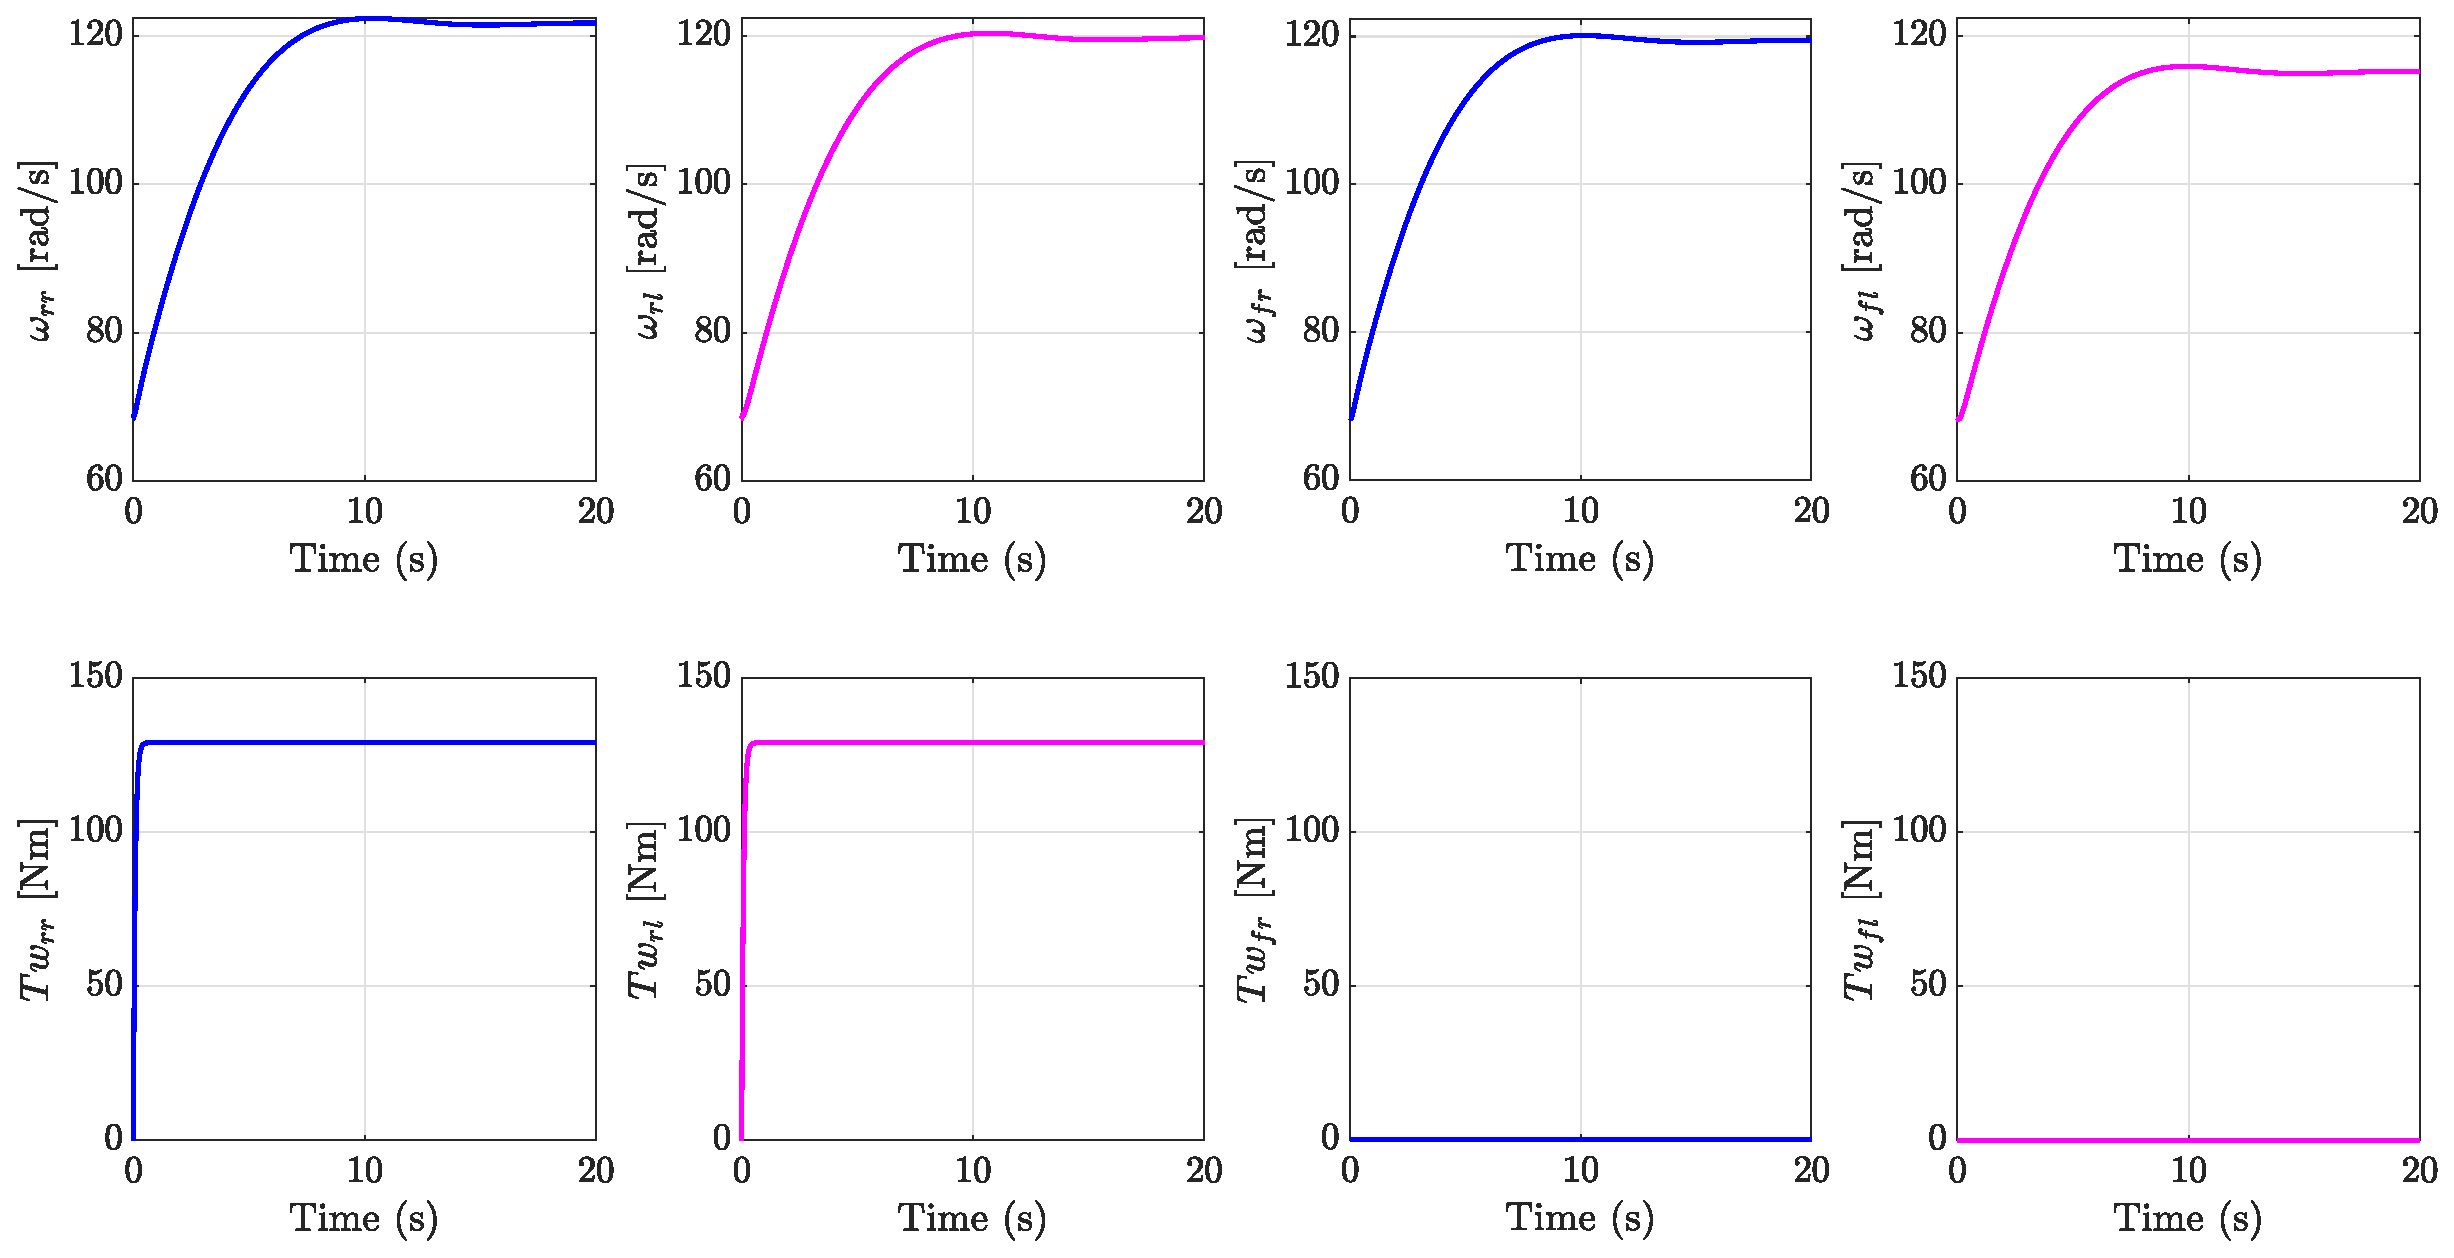
\includegraphics[width=0.88\linewidth]{ex4/q3/ex-43g.eps}
        \centering
        \caption{Wheel rates $\omega$ and Torques $Tw$ [maneuver \#3]}
        \label{43g}
        \end{figure}

The angular velocity $\omega$ are different for different for each wheel as the outer [right] tires would need to rotate faster than the inner [left] tires [Figure \ref{43g}]. The torque experienced by the rear tires are equal to each other, while the front ones are zero.

The longitudinal slip $\kappa$ relies on $\omega$ for each wheel and can be calculated using Equation \ref{eq:4.3}:

\begin{equation}\label{eq:4.3} % add * after equation for unnumbered equations
    \kappa_{ij} = \frac{\omega_{ij} R_{ij} - \upsilon_{cxij} }{\upsilon_{cxij}} \quad i \in \{f,r\} \quad j \in \{r,l\}
\end{equation}

Figure \ref{43f} shows $\kappa$ and $\fx$. As there was no torque on the front tires, $\kappa$ and $\fx$ on the front tires were small. $\kappa$ for the rear tires are different because they are rotating at different speeds. However, both rear tires still experienced the same $\fx$.

        \begin{figure}[ht]
        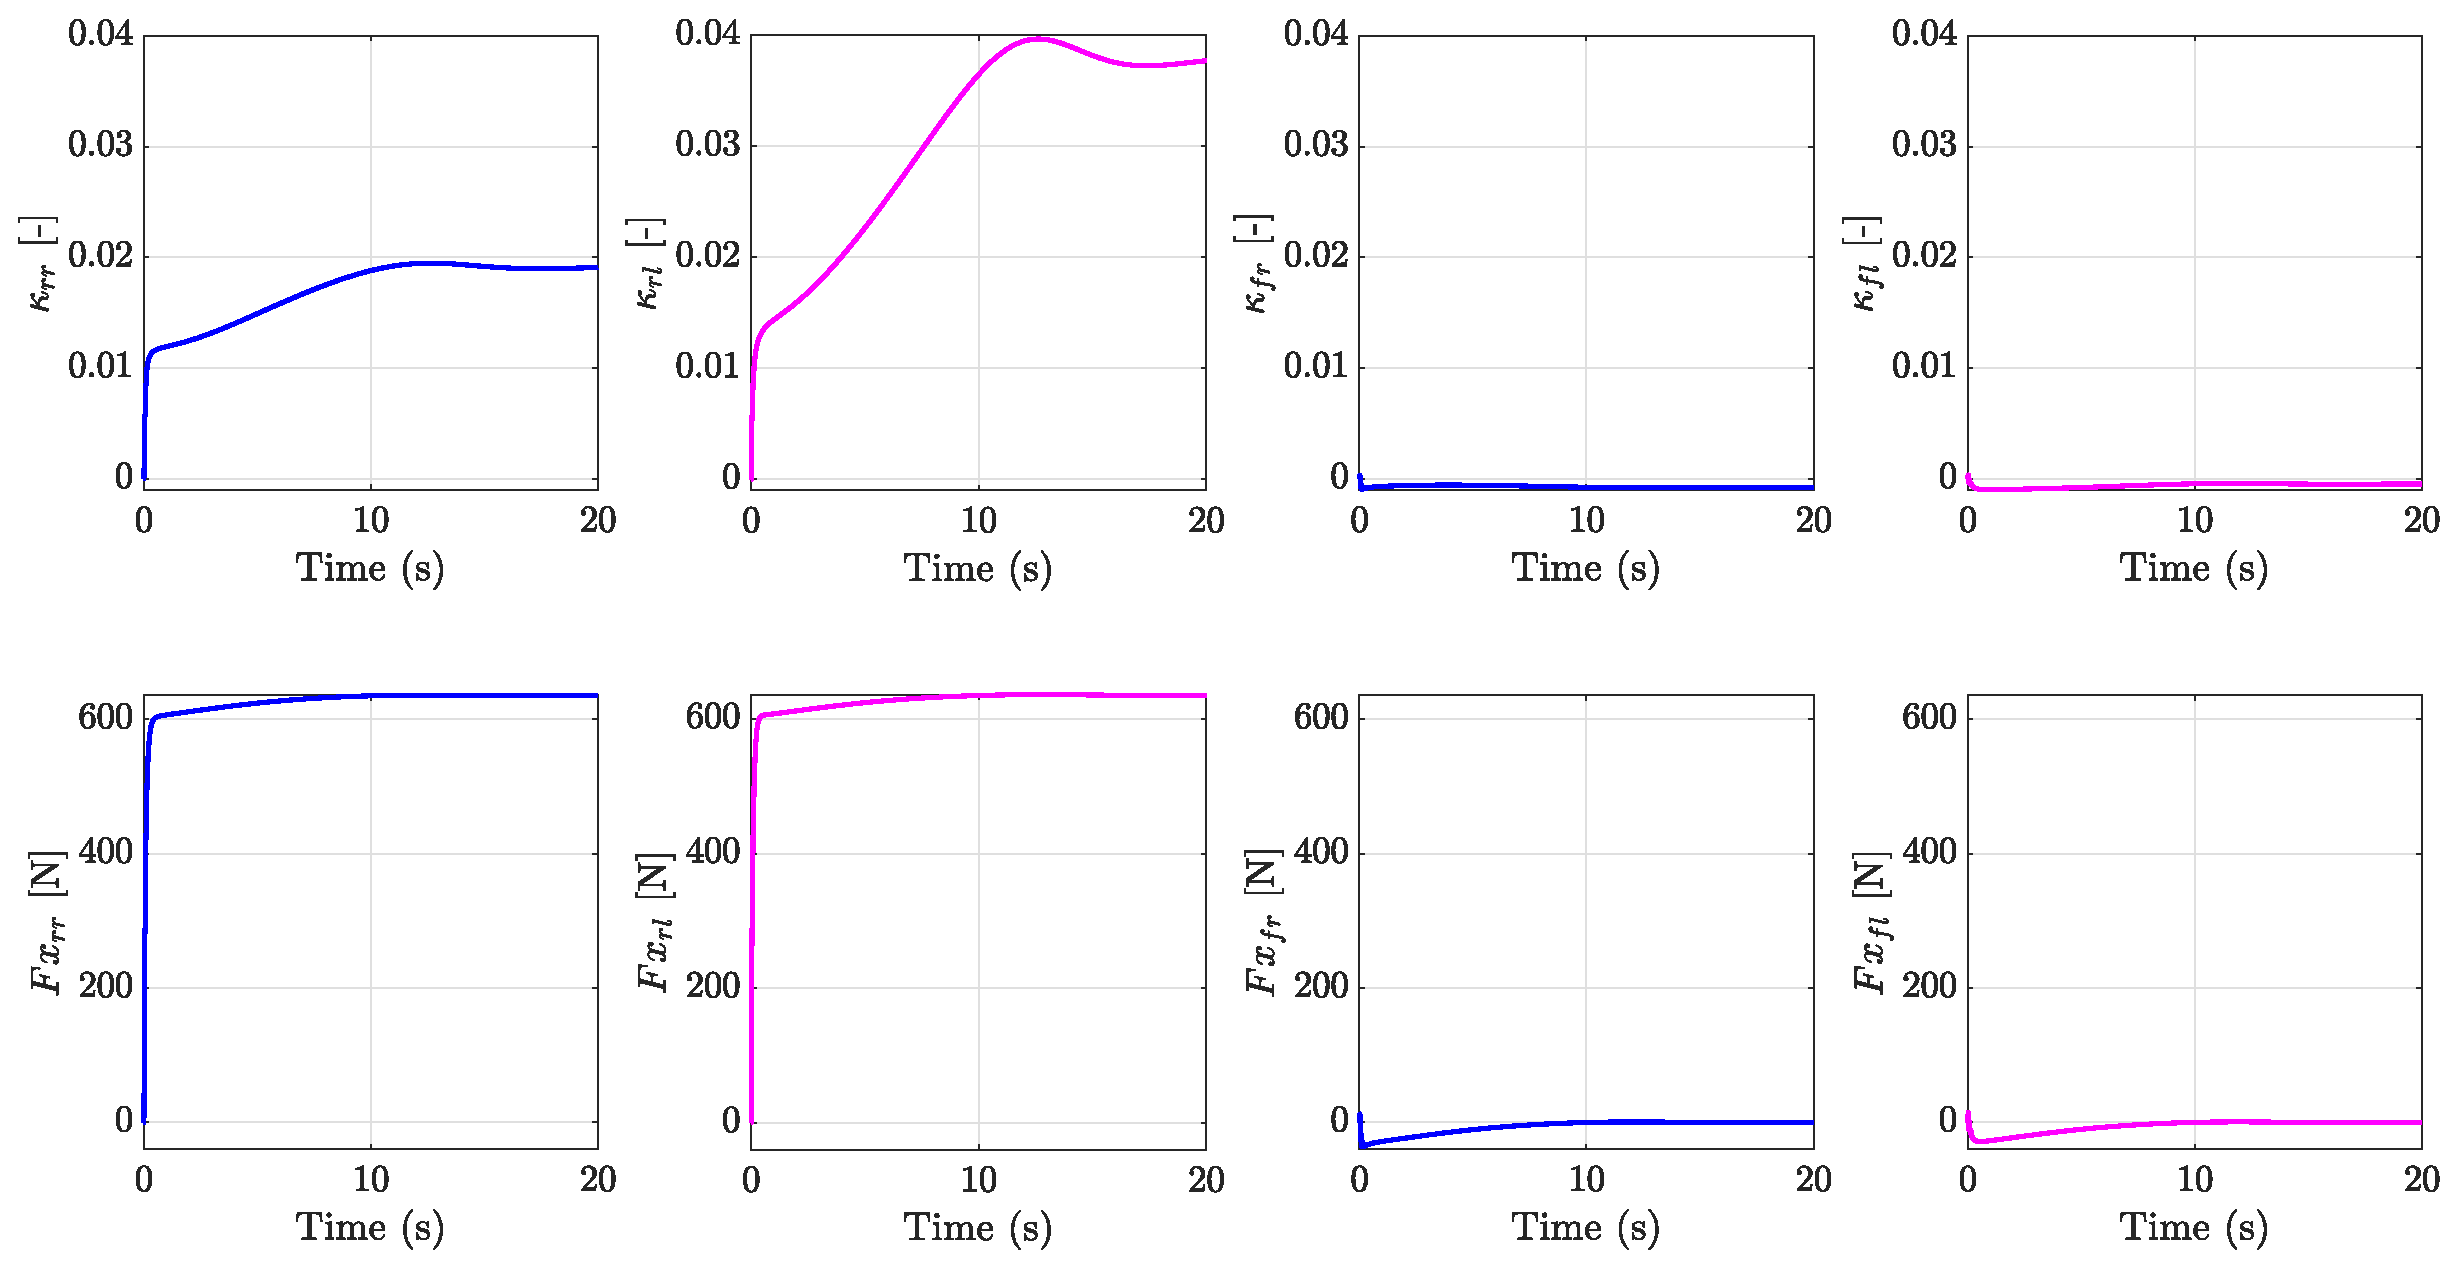
\includegraphics[width=0.88\linewidth]{ex4/q3/ex-43f.eps}
        \centering
        \caption{longitudinal slip $\kappa$ and longitudinal forces $\fx$ [maneuver \#3]}
        \label{43f}
        \end{figure}
        

        \begin{figure}[ht]
        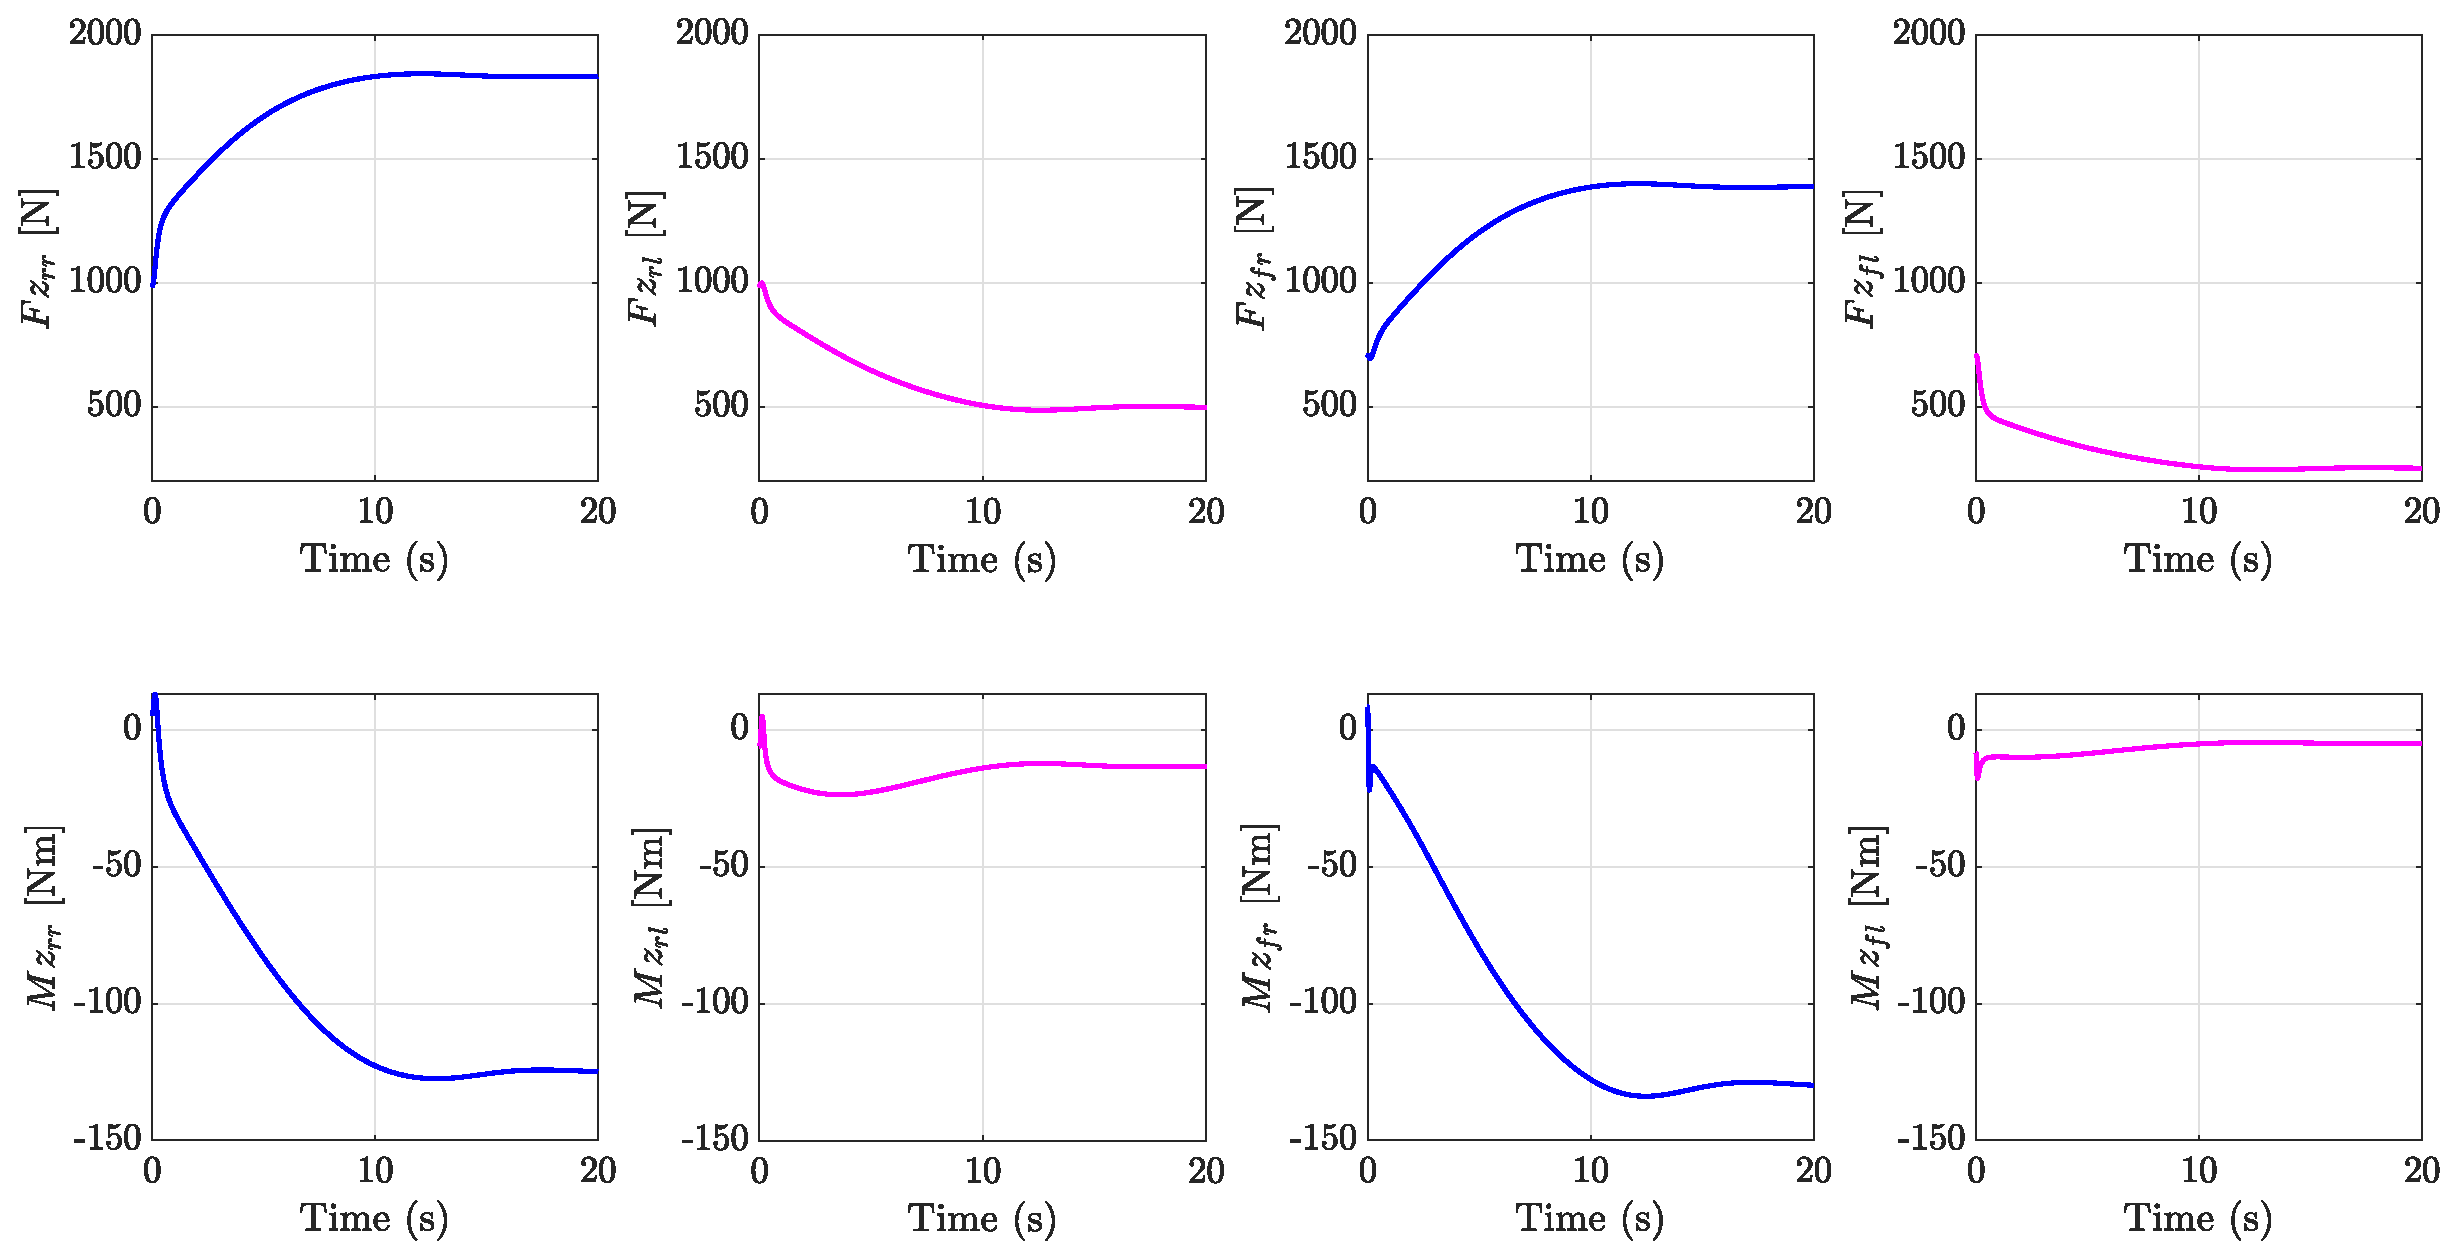
\includegraphics[width=0.88\linewidth]{ex4/q3/ex-43h.eps}
        \centering
        \caption{Vertical forces $\fz$\ and self aligning torque $M_{z}$ [maneuver \#3]}
        \label{43h}
        \end{figure}

Figure \ref{43h} shows the vertical forces $\fz$ for the right [outer] tires increasing then becoming constant when acceleration becomes zero. The left [inner] tires experienced the opposite because of the lateral load transfer to the right side of the vehicle due to the left turn.

The lateral side slip $\alpha$ for all tires are calculated using Equation \ref{eq:4.2}:

\begin{equation}\label{eq:4.2}
    \alpha_{ij} = - \arctan(\frac{vc_{yij}}{vc_{xij}}) \quad i \in \{f,r\} \quad j \in \{r,l\}
\end{equation}

$\alpha$ appears to be consistent across the four tires as shown in Figure \ref{43d}. However, the rear tires are slightly higher due to the torque applied by the motors.

The right side tires have higher lateral forces $\fy$ compared to the right. This is because $\fy$ relies on $\fz$, as the the lateral load transferred to the right side during the left turn maneuver. Both $\alpha$ and $\fy$ become constant once the acceleration is equal to zero. The self aligning torque $\mz$ profiles in Figure \ref{43h} for each tire are trying to counter the $\fy$'s effect on the steering.

        \begin{figure}[ht]
        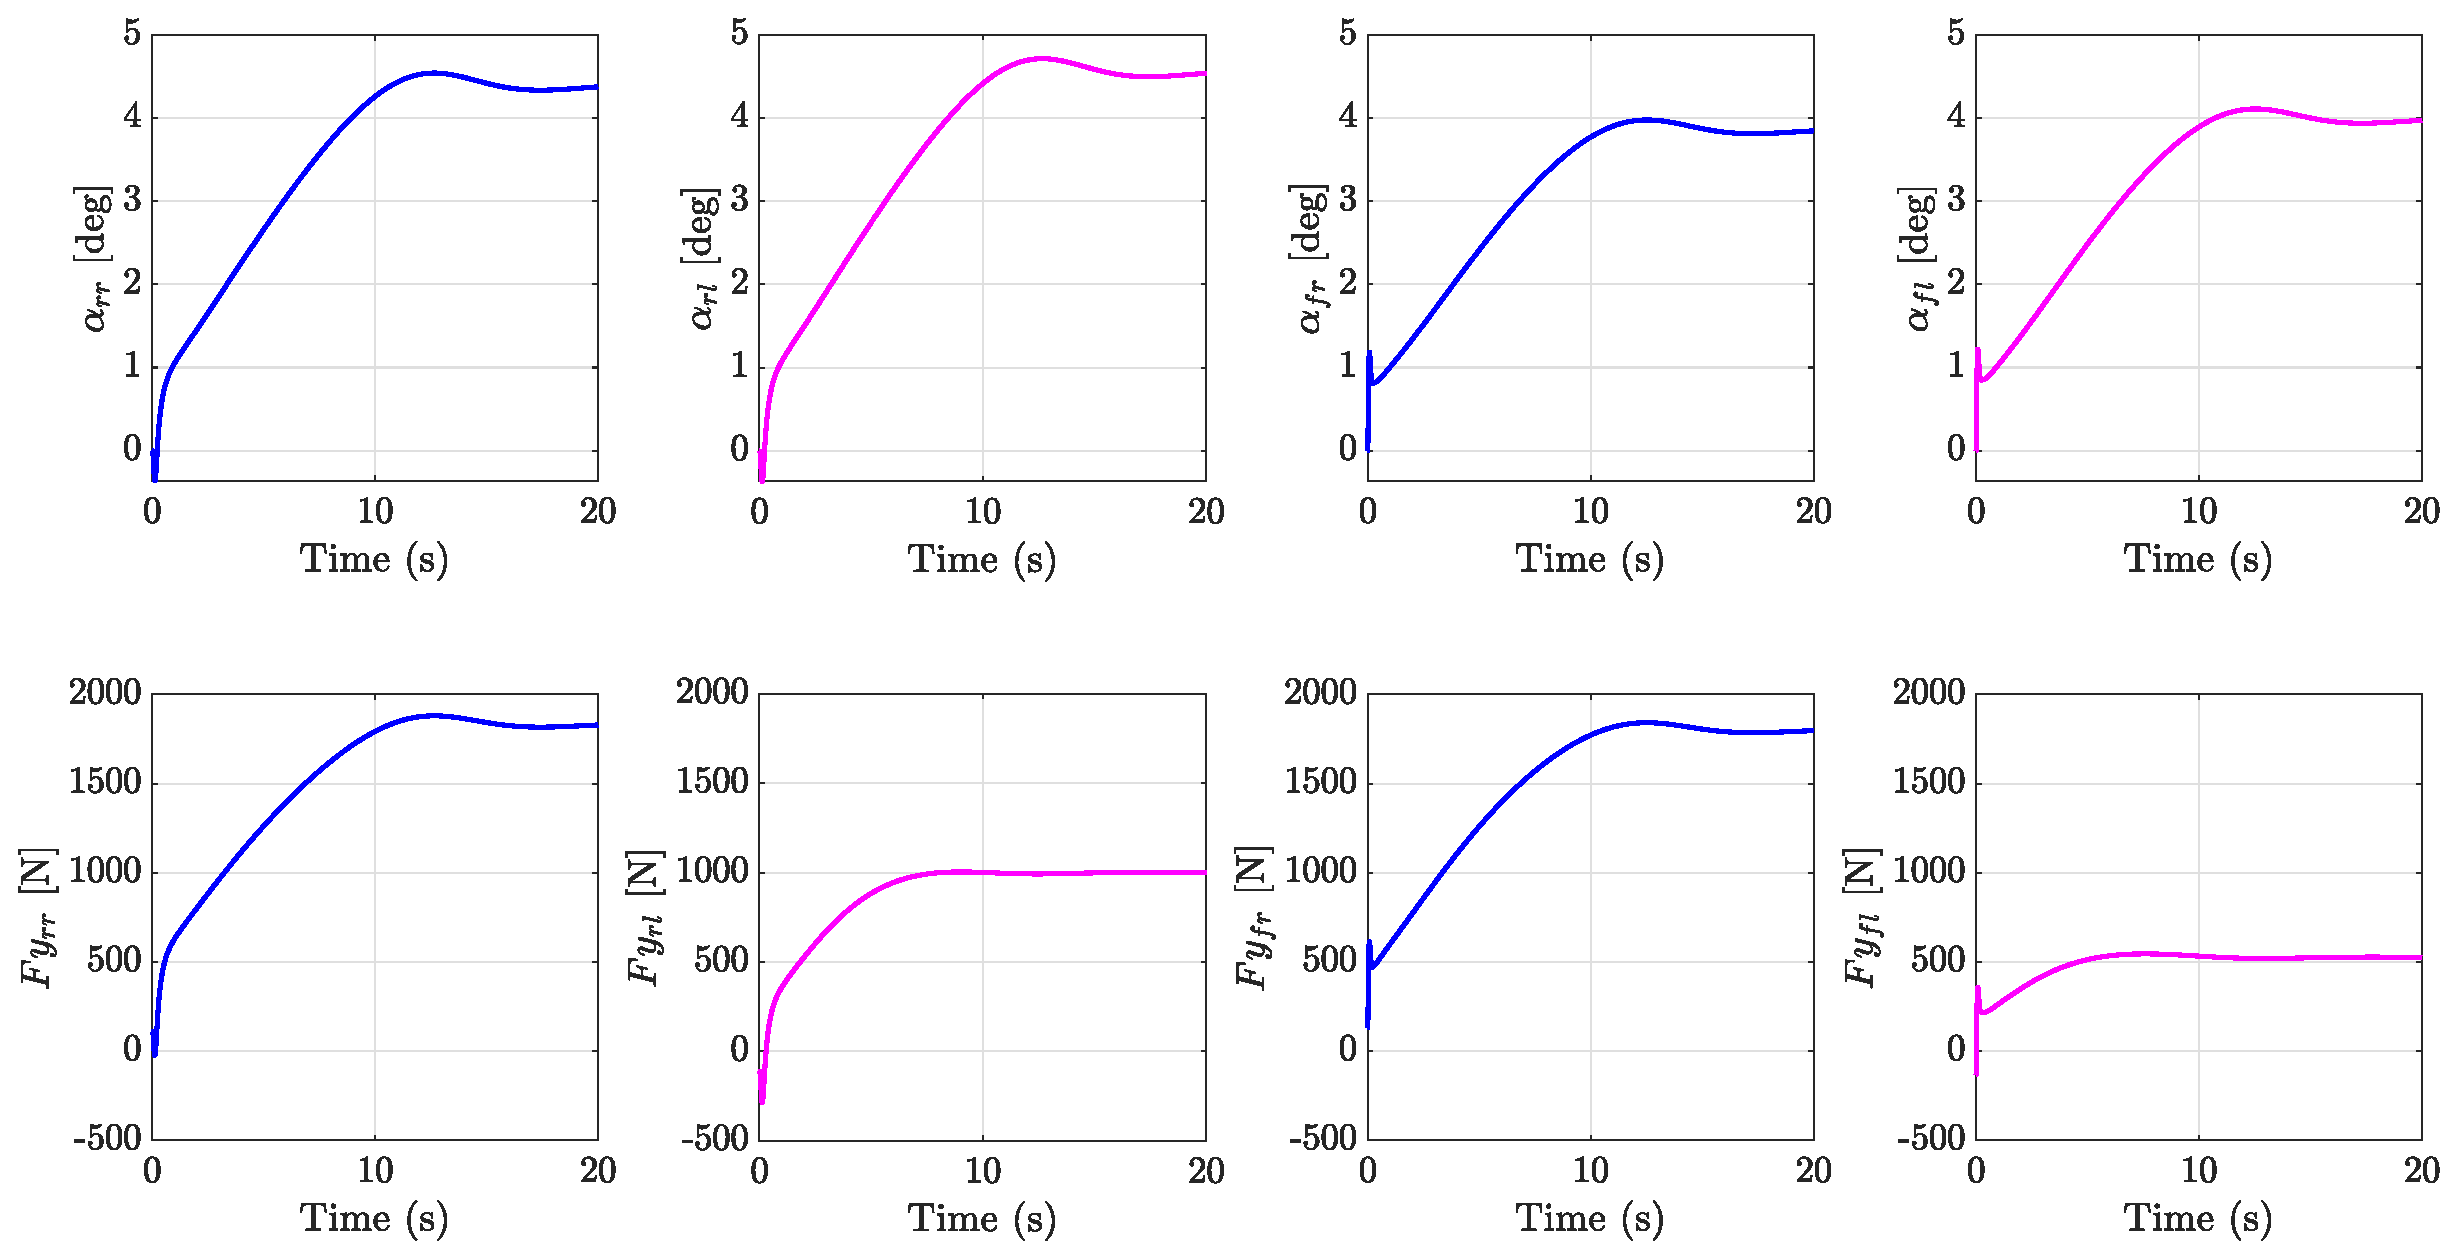
\includegraphics[width=0.88\linewidth]{ex4/q3/ex-43d.eps}
        \centering
        \caption{side slip angle $\alpha$ and lateral forces $\fy$ [maneuver \#3]}
        \label{43d}
        \end{figure}

\chapter{Handling Identification}

\section{Exercise 1 - Sine Steer Maneuvers}

\textbf{Q. Perform a set of sine steer maneuvers, with steering wheel angle $\deltd$\ = $\deltdz$\ $\sin(2\pi ft)$. Use $\deltdz$\ = $5^\circ$, and repeat the test at 3 different u = \{50, 80, 100\} km/h.}

        \begin{figure}[ht]
        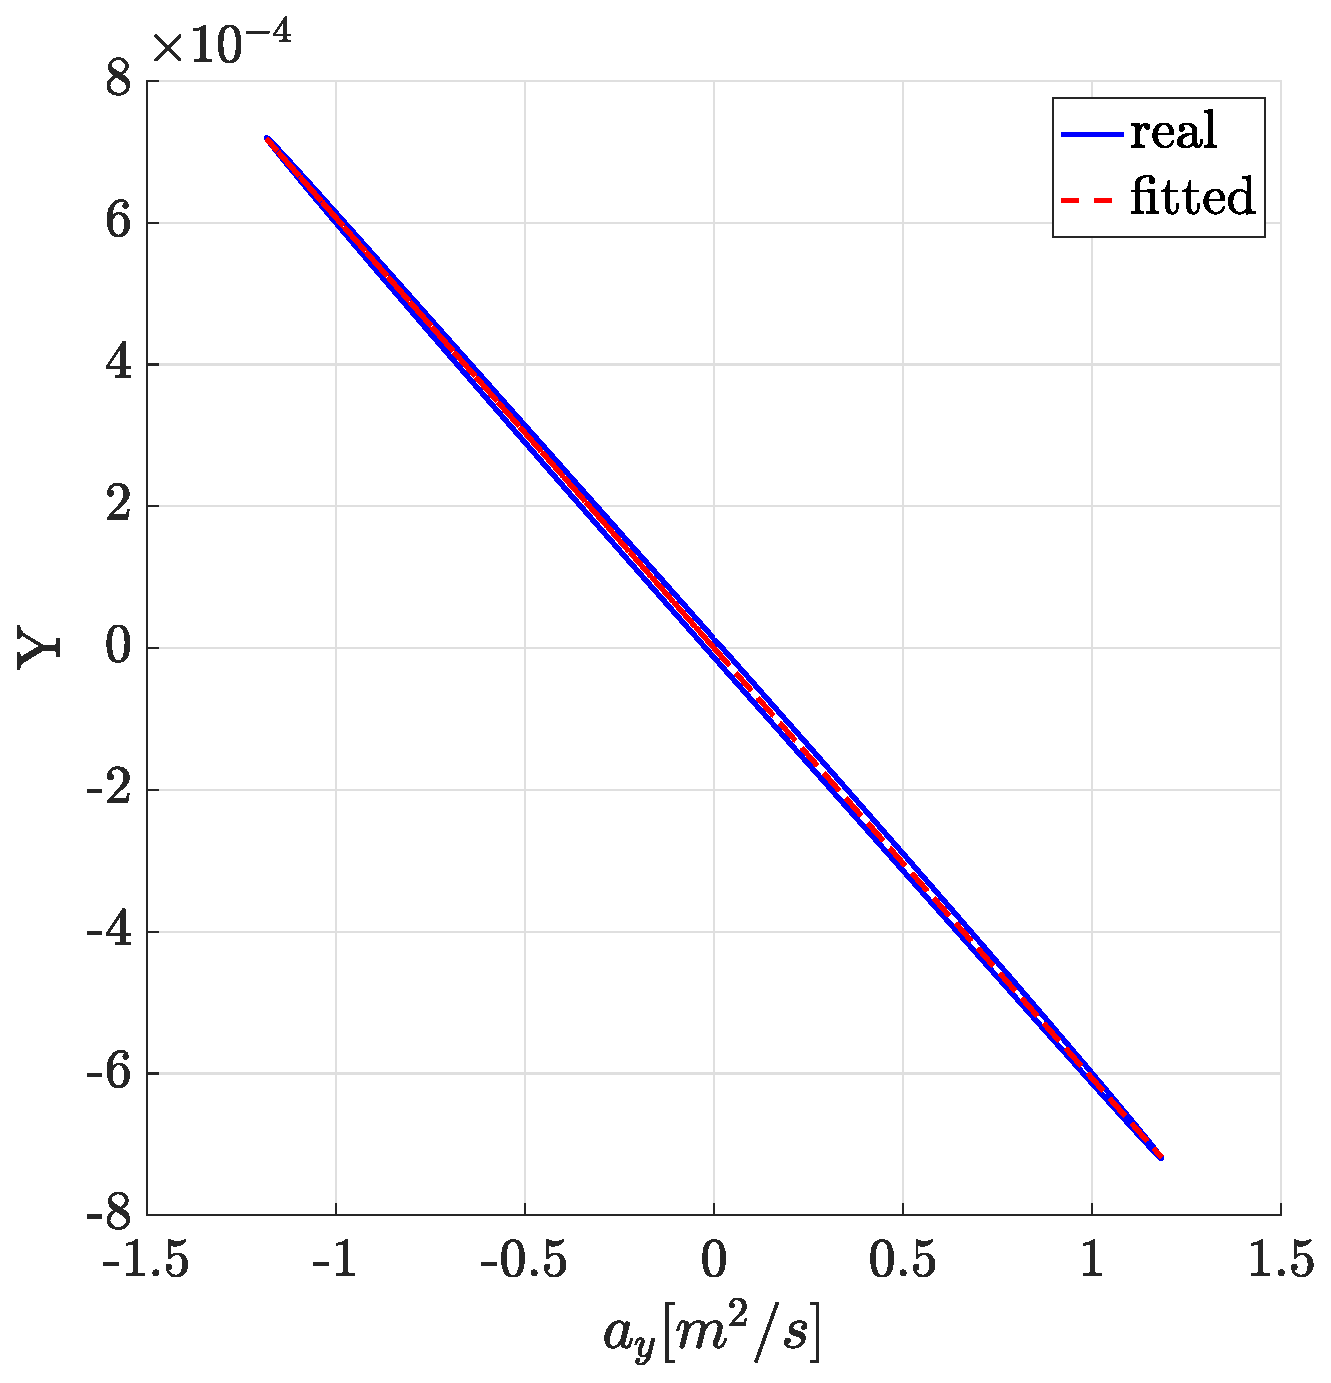
\includegraphics[width=0.5\linewidth]{ex5/q1/ex-51b1.eps}
        \centering
        \caption{Handling diagram result [$\deltdz$\ = $5^\circ$, $u$ = 50 km/h]}
        \label{51b1}
        \end{figure}

Figure \ref{51b1} shows the handling diagram result of a sine steering maneuver that uses a desired steering angle $\deltd$\ = $\deltdz$\ $\sin(2\pi ft)$ at speed 50 km/h. The frequency $f$ in the equation is the number of complete cycles that happen every second. We must perform changes to our system very slowly in order to preserve steady state conditions. The frequency used was $0.001$ $s^{-1}$ and the simulation time was a 1000 s. The  Y refers to the handling behaviour of the vehicle and is calculated using Equation \ref{eq:5.1}:

\begin{equation}\label{eq:5.1}
    Y = \delta - \frac{\Omega}{u} L
\end{equation}

The handling curve obtained at 50 km/h has a negative slope and appears to be linear. The data can be fitted with a first degree polynomial [$f(x) = ax +b$] as shown in Figure \ref{51b1}.

The negative slope indicates that the vehicle exhibits an over-steering behaviour. Over-steering occurs when the vehicle's rear wheels have higher lateral slip compared to the front [$\alpha_{r} > \alpha_{f}$]. This causes the rear wheels to have a larger radius of curvature than the front and the vehicle steers more than expected. If we want to keep the same radius of curvature in an over-steering condition, we must decrease the steering angle $\delta$ at higher velocities.

        \begin{figure}[ht]
        \includegraphics[width=0.99\linewidth]{ex5/q1/ex-51c.eps}
        \centering
        \caption{Handling diagram results at different speeds}
        \label{51c}
        \end{figure}

The slope of the line represents the under-steering gradient $\kus$. It describes the evolution of $\delta$ as $\ay$ increases. $\kus$ is positive if the vehicle is under-steering and negative when over-steering.

Increasing the speeds to 80 and 100 km/h resulted in an increase in the lateral acceleration $\ay$ as shown in Figure \ref{51c}. The vehicle nonetheless showed over-steering behaviour across all the simulated speeds. A comparison between the yaw-rate $\Omega$ and the desired steering angle $\deltd$ shows that the $\Omega$ keeps increasing with higher speeds while $\deltd$ does not.

        \begin{figure}[ht]
        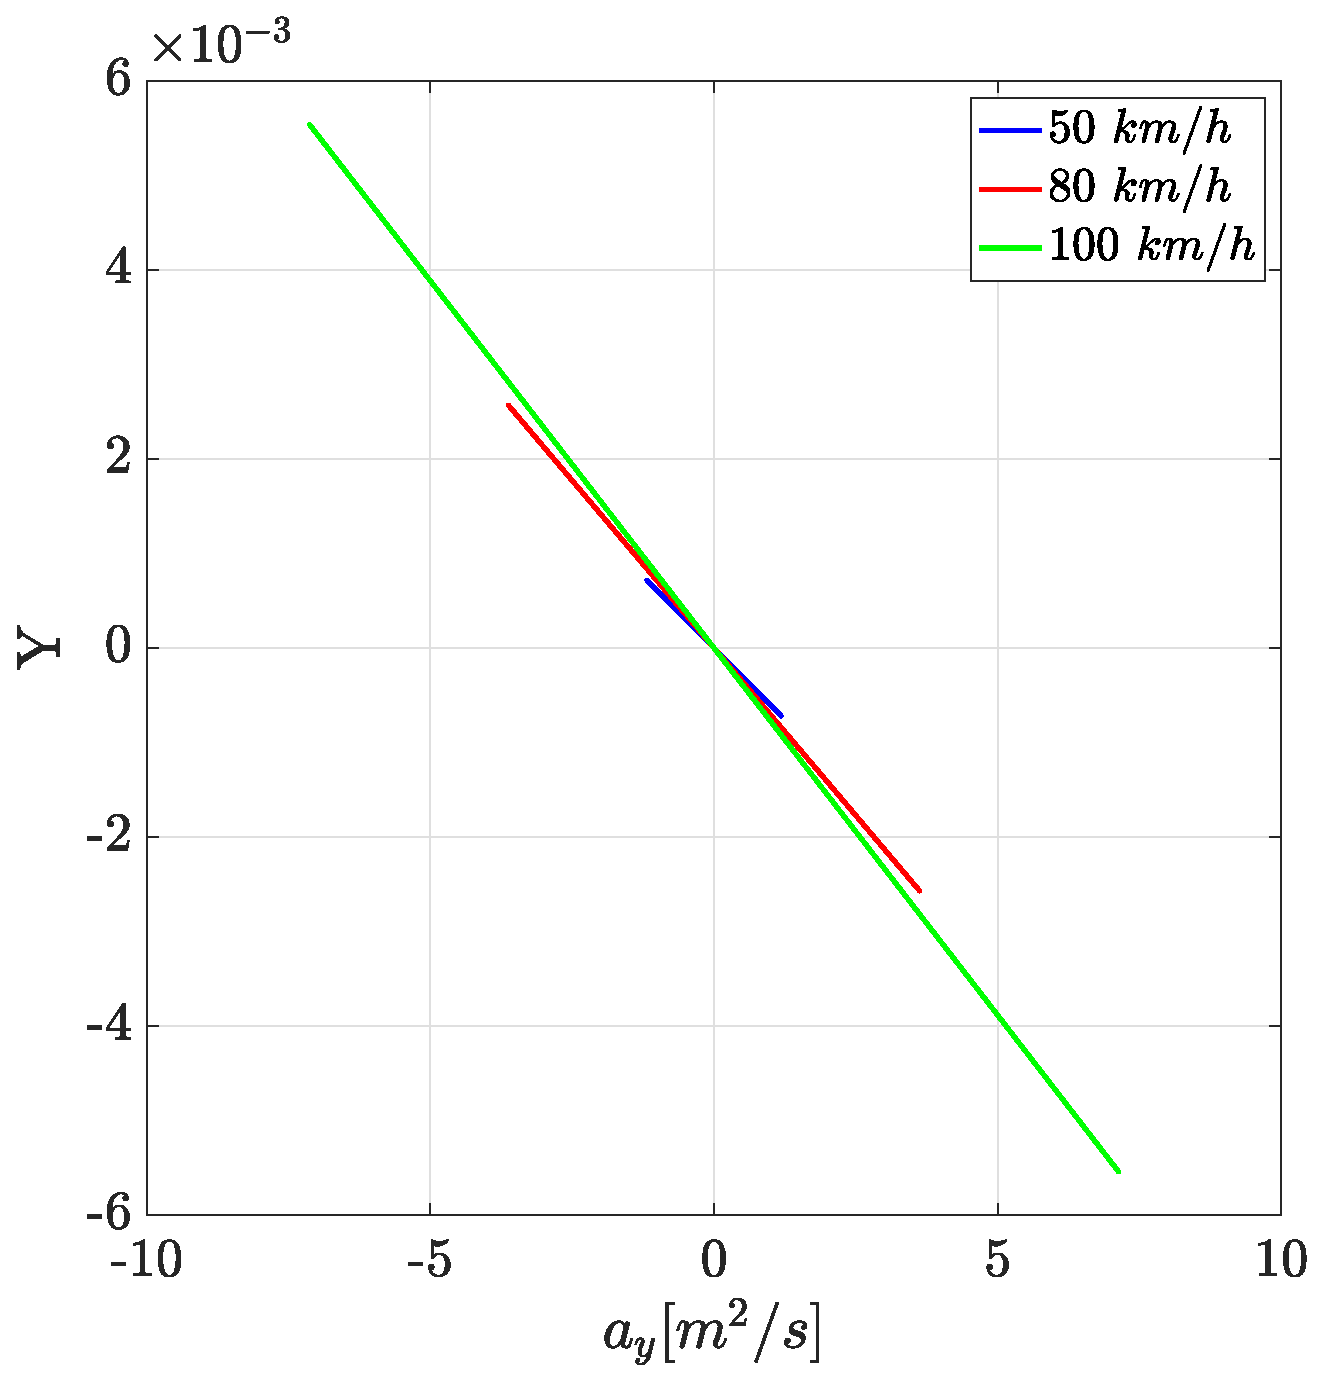
\includegraphics[width=0.6\linewidth]{ex5/q1/ex-51d.eps}
        \centering
        \caption{Handling curve comparison}
        \label{51d}
        \end{figure}
        
Superimposing the handling curves of the three simulated speeds in Figure \ref{51d} clearly shows that with higher speeds, the over-steering behavior increases [steeper negative slope]. That means $\delta$ will need to be decreased even further with higher speeds to keep the same curvature. Furthermore, the obtained curves pass through the origin. That means when there is no lateral acceleration $\ay$, the steering behaviour will be neutral. 

        \begin{figure}[ht]
        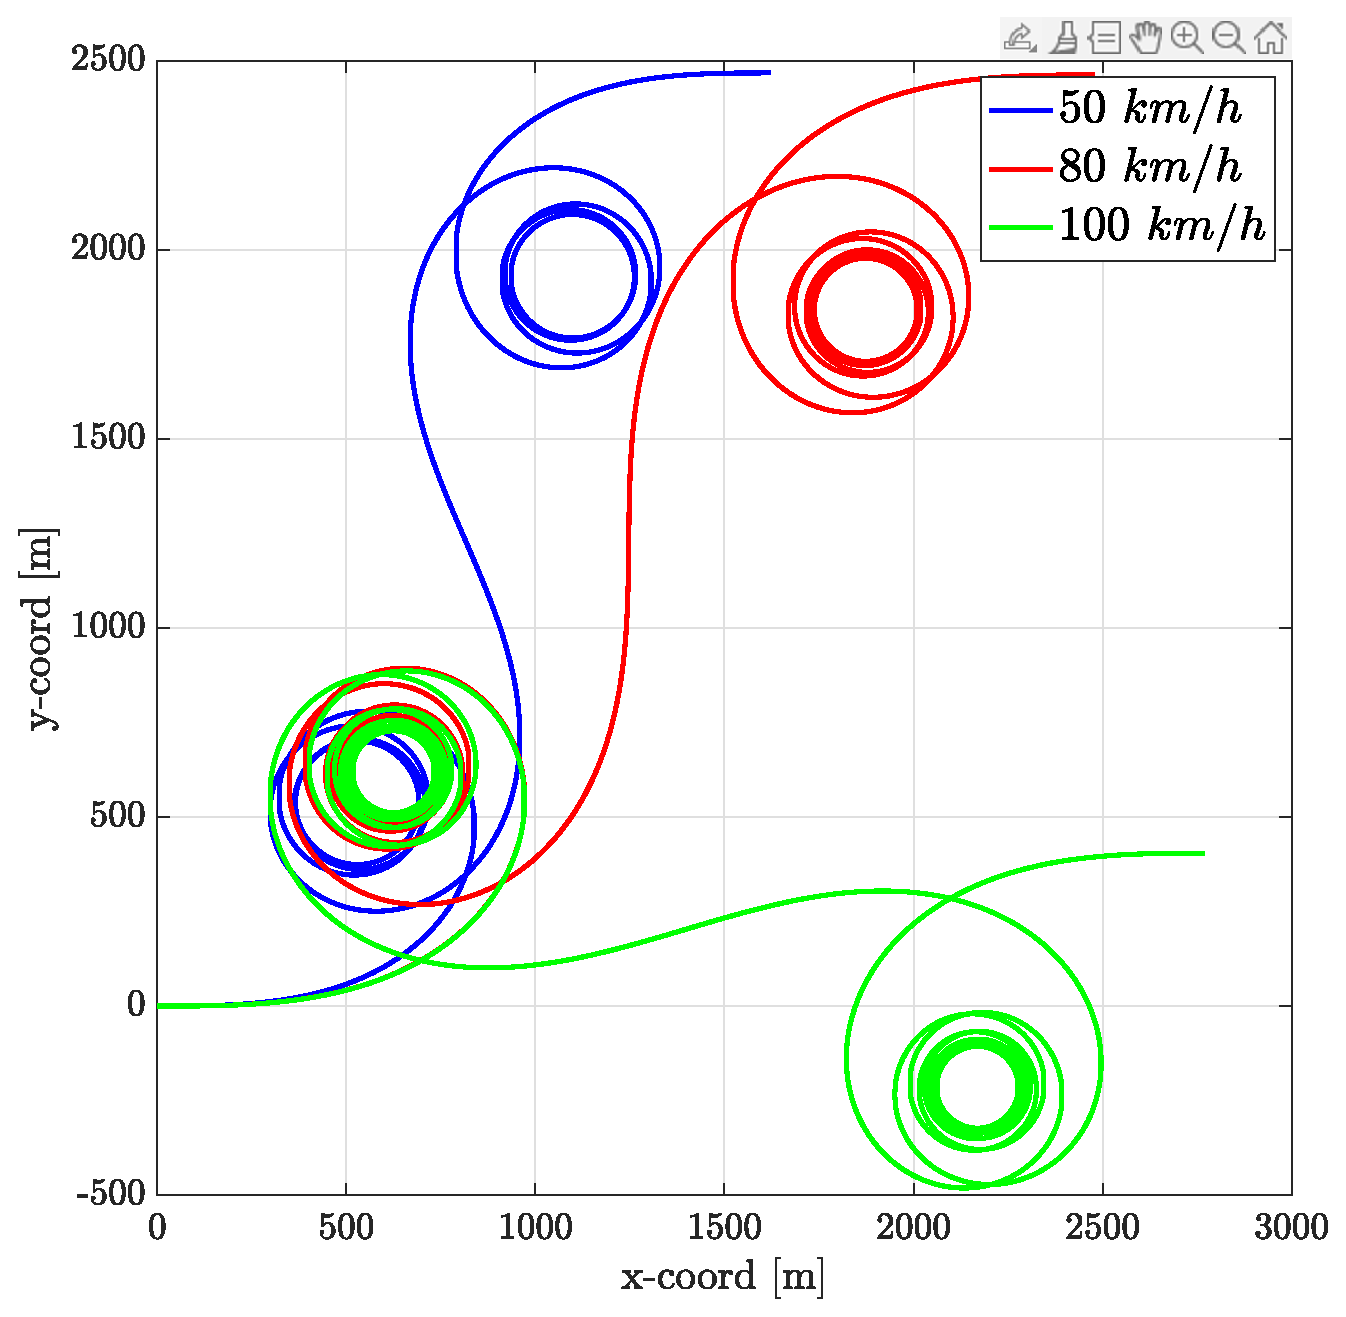
\includegraphics[width=0.6\linewidth]{ex5/q1/ex-51a.eps}
        \centering
        \caption{Vehicle paths for sine steer maneuvers at different speeds}
        \label{51a}
        \end{figure}
        
Plotting the path results of the three different speeds, as shown in Figure \ref{51a}, confirms the over-steering behaviour. The radius of the curvature [the size of the circles] decreases with increasing velocities.

\textbf{Q. carry out other 3 sine steer maneuvers, with these data: \vspace{-1em}
\begin{enumerate}
    \item \boldmath$\deltdz$ = $70^\circ$ , $u$ = 50 km/h
    \item $\deltdz$ = $24^\circ$ , $u$ = 80 km/h
    \item $\deltdz$ = $12^\circ$ , $u$ = 100 km/h
\end{enumerate}}

\section{Exercise 2 - Constant Steer Maneuvers}

\chapter{Lateral Control}

\section{Exercise 1 - lateral control}
\textbf{Q. Optimize the clothoid-based lateral controller}

The clothoid-based lateral controller uses Equation \ref{eq:6.1} to calculate the steering angle required to follow the clothid. The under-steering gradient $\kus$ was calculated previously using the handling diagram shown in Table \ref{tab:5.1}. These results were implemented as a variable that changes based on the vehicle's current speed.

\begin{equation}\label{eq:6.1}
\delta(s) = k(s) (L + \kus u^2)
\end{equation}

To optimize the clothoid-based lateral controller look ahead variable, several tests were conducted using the following variables totalling 42 tests:

\begin{itemize}
    \item $u$ = [10, 20, 30, 40, 50, 60, 70, 80] km/h
    \item look ahead = [5, 10, 15, 20, 25, 30]
\end{itemize}

The tracking error had to be calculated to compare the tests' results. That was done by using the ``N-D nearest point search" function in Matlab, which returns indices of closest points in the desired path for each point on the real path. Then calculating the euclidean distance between each point in the real path and closest point on the desired path as tracking error. The results are shown in Figure \ref{61a-4} and Table \ref{tab:6.1} where LA is the look ahead value.
        
        \begin{figure}[ht]
        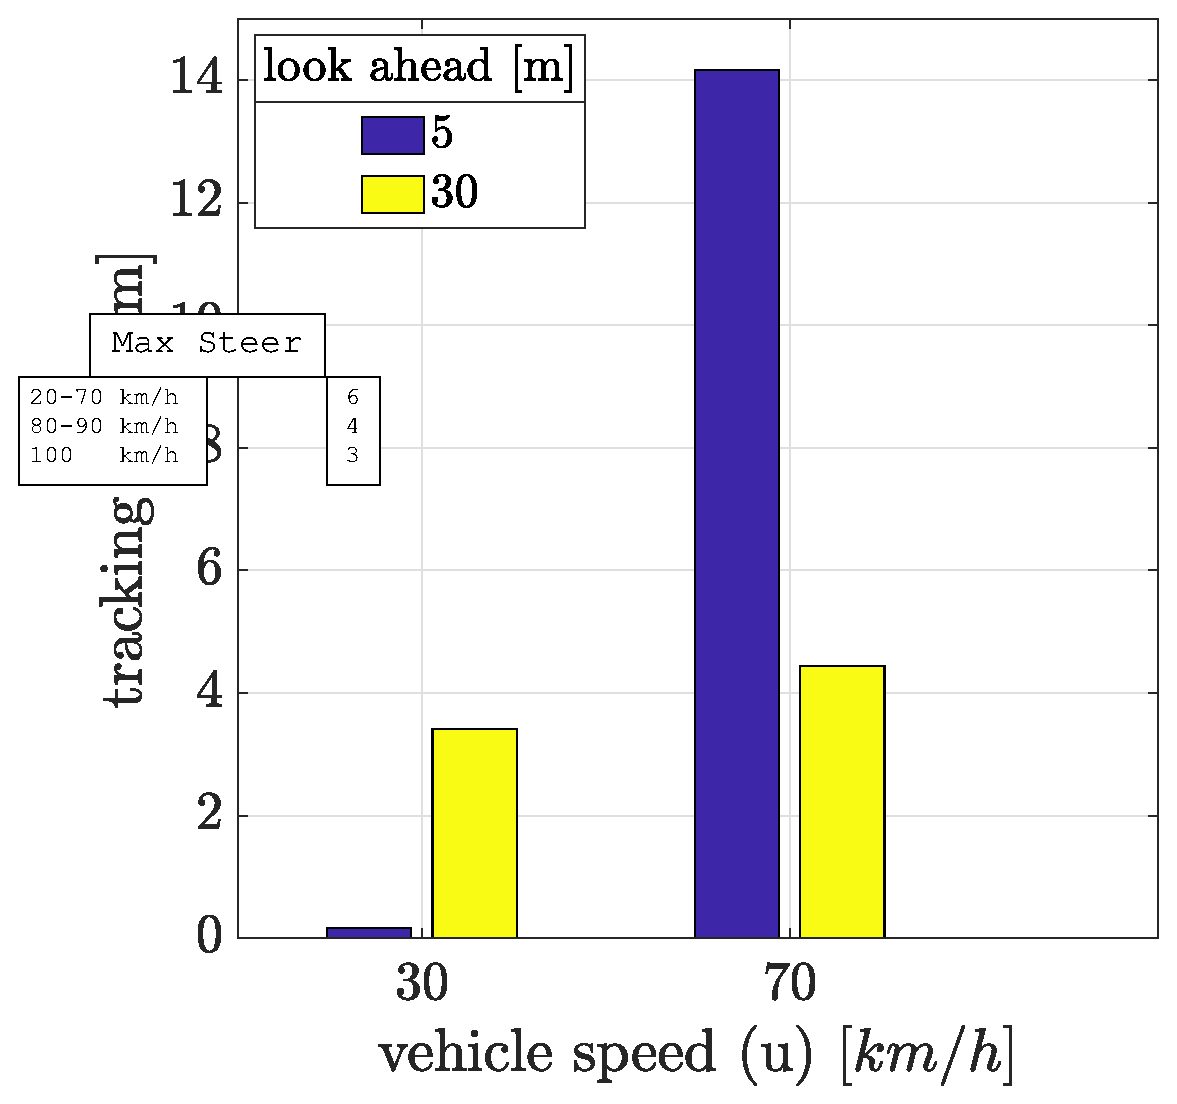
\includegraphics[width=0.6\linewidth]{ex6/q1/ex-61a-4.eps}
        \centering
        \caption{clothoid-based lateral controller at different $u$ and look ahead}
        \label{61a-4}
        \end{figure}
      
The tests checked if the vehicle was able to arrive at a designated target point chosen to be at [60,10]. If the vehicle reaches this point within a threshold of 5 meters, the test is considered a success.

\begin{table}[ht]
    \centering
    \begin{tabular}{c | c | c| c | c | c | c }
      \textbf{$u$ [km/h]} & \textbf{LA = 5} & \textbf{LA = 10} & \textbf{LA = 15} & \textbf{LA = 20} & \textbf{LA = 25} & \textbf{LA = 30} \\ \hline
      20 &  \cellcolor{green!10}\num{0.212718999}	& \num{0.481794113}	& \num{1.025936442} &	\num{1.72651936}	& \num{2.534489657}	& \num{3.45986332}   \\\hline
      30 &  \cellcolor{green!10}\num{0.163715271} &	\num{0.431919243} &	\num{0.941254925} &	\num{1.632800857} &	\num{2.454559877} &	\num{3.408670041}\\\hline
      40 &  \cellcolor{green!10}\num{0.225603124} & \num{0.361992743}	& \num{0.728903508} &	\num{1.387858567} &	\num{2.228111216} &	\num{3.252073013}  \\\hline
      50 & \cellcolor{red!10}NA & \num{9.077008353} & \num{1.421928047} & \cellcolor{green!10}\num{0.718803621} &	\num{1.593478851} & \num{2.81030173} \\\hline
      60 &  \cellcolor{red!10}NA & \num{12.14781879} &	\num{8.667722795}	& \cellcolor{green!10}\num{3.2567} & \num{5.819637} & \num{9.074008} \\\hline
      70 &  \num{14.15735028} & \num{23.03289356} & \cellcolor{red!10}NA & \cellcolor{red!10}NA & \num{4.14466} & \cellcolor{green!10}\num{4.4459637}

    \end{tabular}
    \caption{Tracking error results [clothoid-based lateral controller]}
    \label{tab:6.1}
\end{table}

The red colored cells indicates the vehicle was not able to arrive at the designated target point. Green cells are the chosen look ahead values at each speed $u$.

It appears that the larger the look ahead value, the larger the tracking error as expected. Having a larger look ahead at 20 km/h could be beneficial if we are optimizing for traveled distance, and smoother turns [less jerk].

Figure \ref{61x20} shows the vehicle actual path at each look ahead value for 20 km/h tests. A larger look ahead optimized the vehicles path to take a shorter route and take better turns. However, this caused the tracking error to increase, because we are not following the reference trajectory anymore.

       \begin{figure}[ht]
        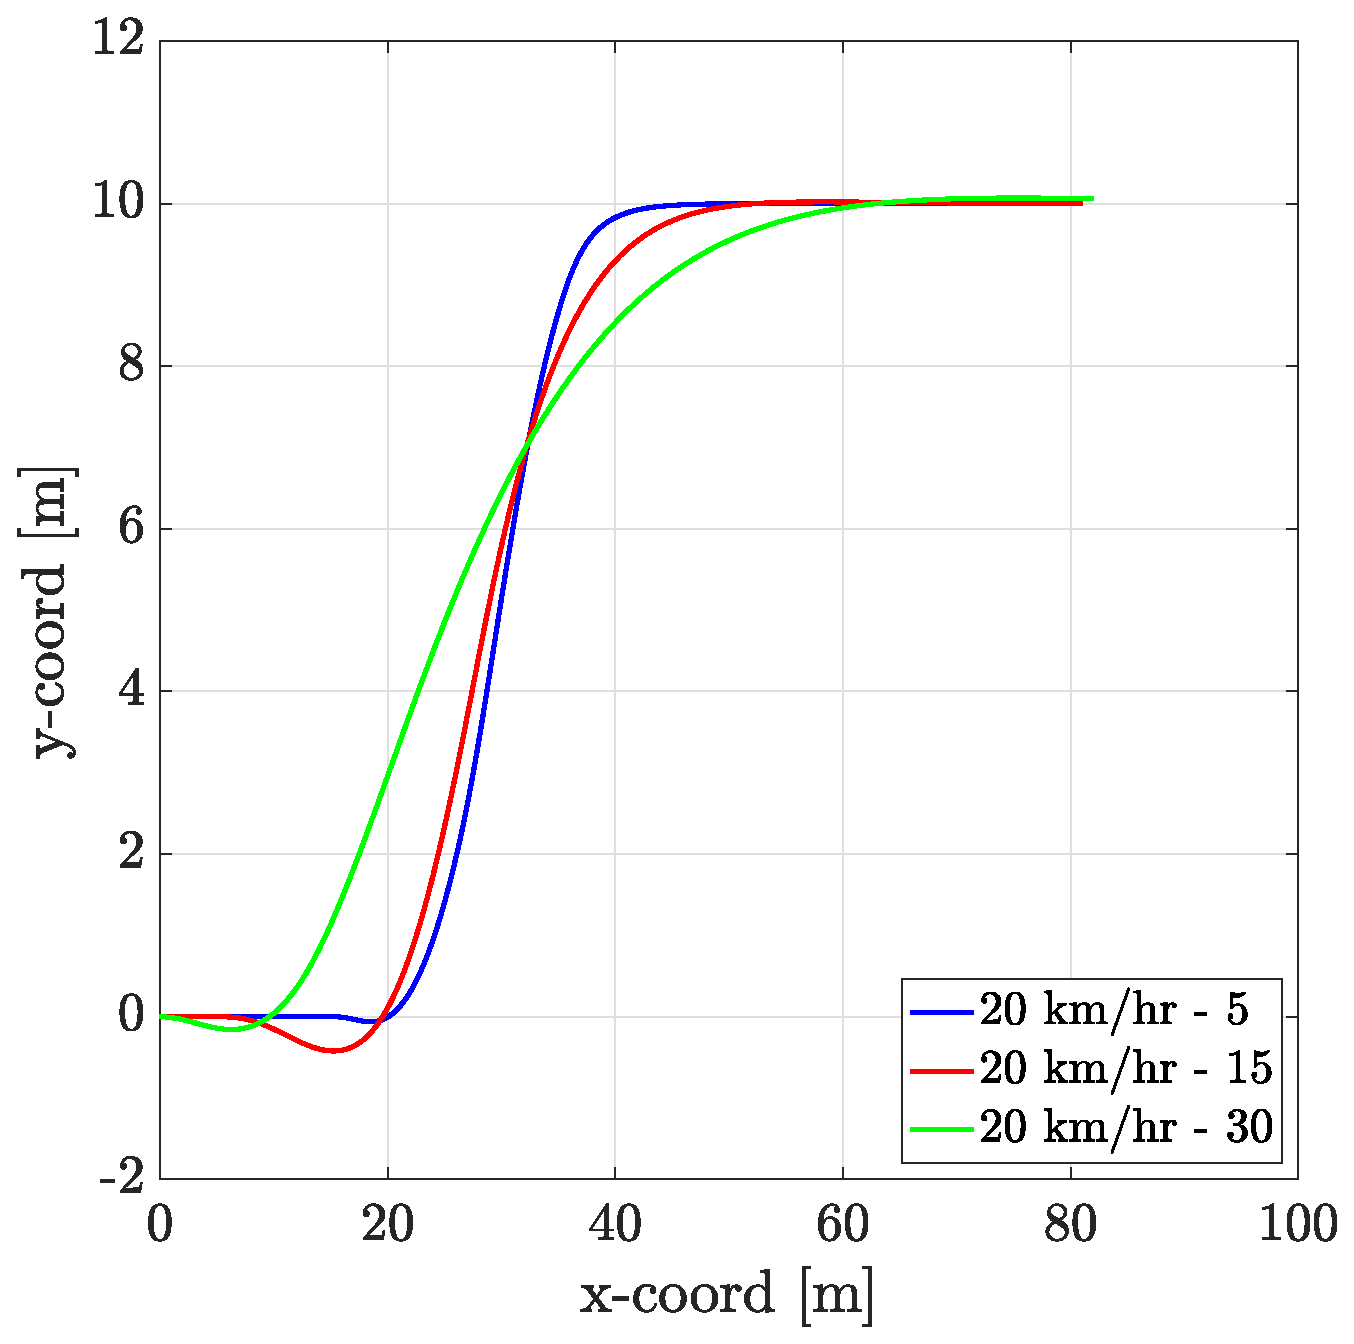
\includegraphics[width=0.6\linewidth]{ex6/q1/ex-61x20.eps}
        \centering
        \caption{Real vehicle path with different look ahead values [$u$ = 20km/h] }
        \label{61x20}
        \end{figure}

Up until 40 km/h, a lower look ahead value performed better for our metrics. With increasing $u$, the smaller look ahead values were simply not enough to control the vehicle properly. The controller needs to see far enough ahead to account for a curve earlier on. The faster the vehicle, the bigger the needed look ahead value. However, it seems that after 70 km/h, the vehicle can no longer become stable even with a look ahead as high as 250. 

Figure \ref{61x70} shows the vehicle paths at 70 km/h at different values for the look ahead. The higher values are more stable but still considered outside the capabilities of the vehicle.

No values of look ahead was enough to stabilize the vehicle with any speed higher than 70 km/h. This might be attributed to the $\kus$ values not being accurate enough at these speeds. The handling curves during these speeds were not linear anymore and a linear approximation for them is not sufficient.

        \begin{figure}[ht]
        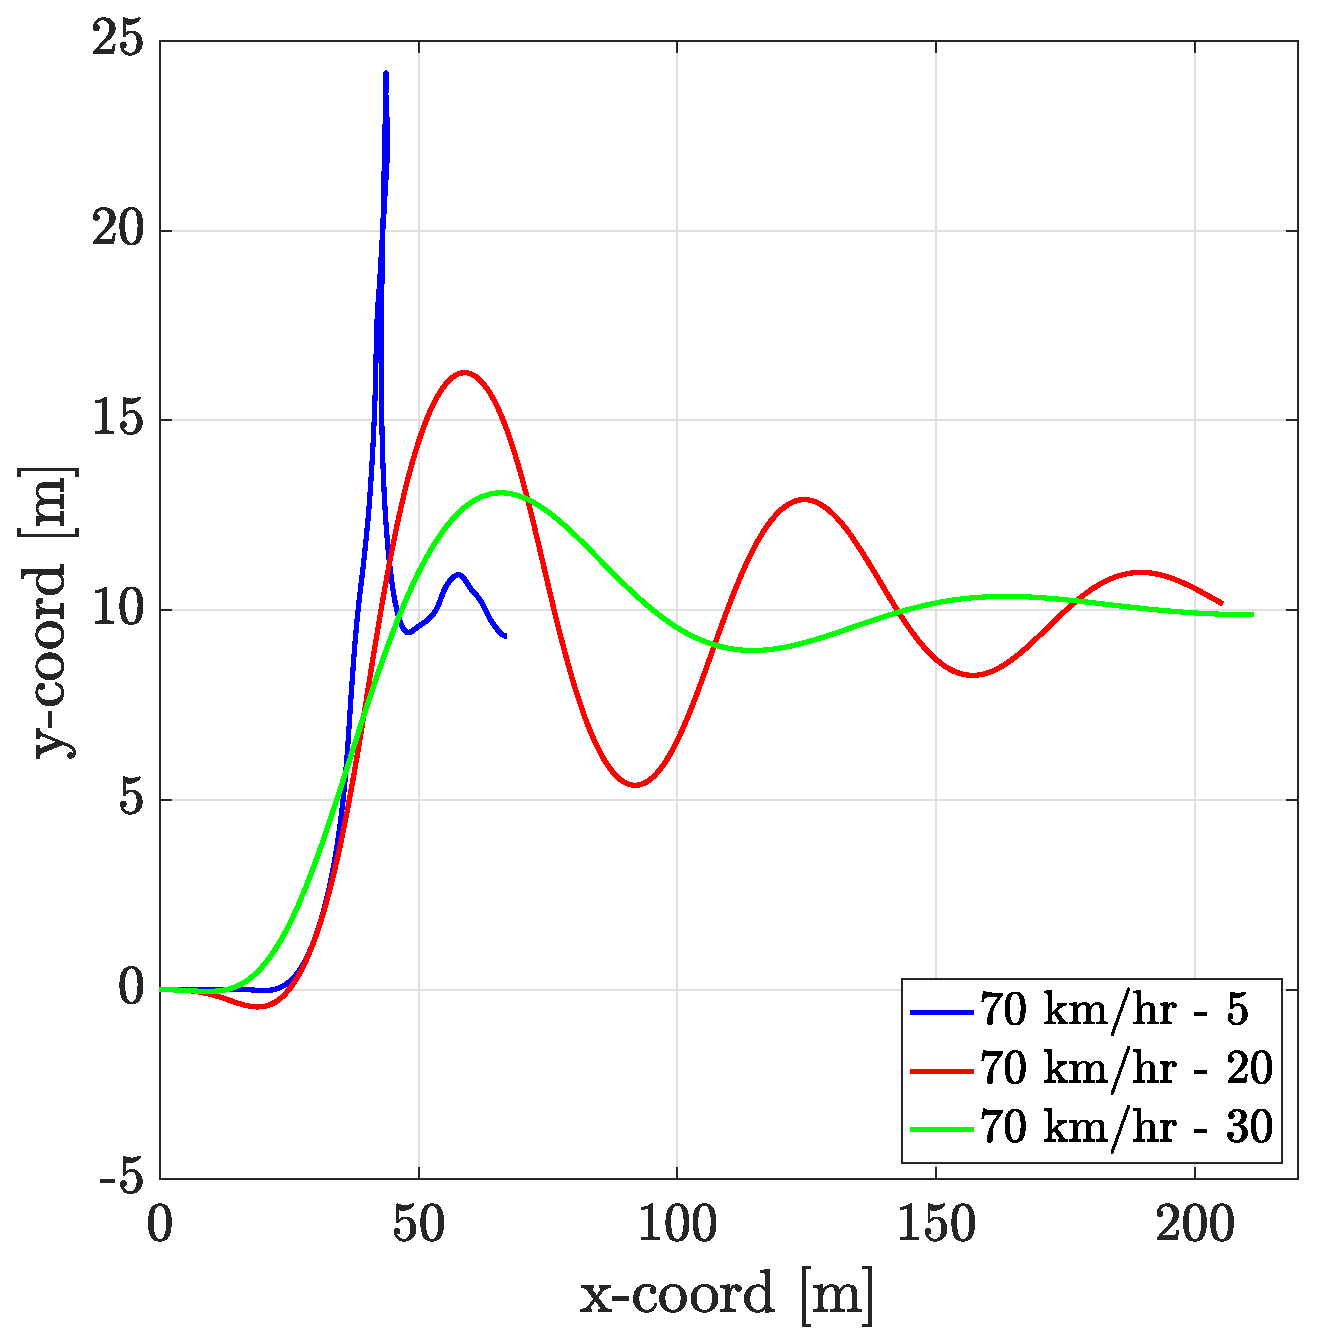
\includegraphics[width=0.6\linewidth]{ex6/q1/ex-61x70.eps}
        \centering
        \caption{Real vehicle path with different look ahead values[$u$ = 70km/h] }
        \label{61x70}
        \end{figure}

\textbf{Q. Implement the pure pursuit controller and optimize the look ahead distance}      

Pure pursuit calculates the circular arc radius $R$ between center of the vehicle's rear wheel $P_{V}$ and the target point on the desired path $P_{D}$. Equation \ref{eq:6.2} is used to calculate $R$, where $x_{D} $ and $y_{D}$ are $P_{D}$ expressed in the vehicle's frame. $R$ is later used to calculate the required steering angle $\delta$.

\begin{equation}\label{eq:6.2}
R = \frac{\sqrt{x_{D}^2 + y_{D}^2}}{2 sin(\lambda)} \quad\mathrm{and}\quad \delta = arctan(L/R)
\end{equation}

To optimize the pure pursuit lateral controller look ahead variable, several tests were conducted using the following variables totalling 64 tests:

\begin{itemize}
    \item $u$ = [20, 30, 40, 50, 60, 70, 80, 90, 100] km/h
    \item look ahead = [1, 2, 3, 4, 5, 10, 15, 20, 25, 30]
\end{itemize}

The tracking error was calculated in the same manner as previous and some of the results are shown in Figure \ref{62a-1} and Table \ref{tab:6.2}. The effect of the look ahead variable on the pure pursuit controller behaviour is similar to the clothoid-based controller. With higher speeds, larger look ahead values are required.
        \begin{figure}[ht]
        \includegraphics[width=0.6\linewidth]{ex6/q2/ex-62a-1.eps}
        \centering
        \caption{pure pursuit lateral controller at different $u$ and look ahead}
        \label{62a-1}
        \end{figure}

Overall, the pure pursuit controller performed well. Table \ref{tab:6.2} shows some of the tests conducted and their tracking error. The red colored cells indicate the vehicle was not able to arrive at the target point, while the green cells are the best performers for each speed $u$. A look-up table can now be used to choose the correct look ahead based on current speed.

\begin{table}[ht!]
    \centering
    \begin{tabular}{c | c | c| c | c | c | c }
      \textbf{$u$ [km/h]} & \textbf{LA = 3} & \textbf{LA = 10} & \textbf{LA = 15} & \textbf{LA = 20} & \textbf{LA = 25} & \textbf{LA = 30} \\ \hline
      20 &  \cellcolor{green!10}\num{0.122447479884261}	& \num{1.20229858149544}	& \num{1.98665627365860} &	\num{2.50901222735532}	& \num{2.89607564298269}	& \num{3.36310387417133}   \\\hline
      40 &  \cellcolor{green!10}\num{0.545850027367760} &	\num{0.903114425955597} &	\num{1.73093343366169} &	\num{2.31062509178793} &	\num{2.73594362776234} &	\num{3.23567396181456}\\\hline
      60 &  \num{14.9833184394890} & \num{14.9378800339917}	& \num{11.62915169313966} &\cellcolor{green!10}	\num{2.05379295557061} &	\num{2.47442576799508} &	\num{3.02057477231781}  \\\hline
      80 & \cellcolor{red!10}NA & \cellcolor{red!10}NA & \cellcolor{red!10}NA & \cellcolor{green!10}\num{2.76118476320162} &	\num{2.61057892579461} & \num{3.06265625323397} \\\hline
      100 &  \cellcolor{red!10}NA & \cellcolor{red!10}NA &	\cellcolor{red!10}NA & \cellcolor{red!10}NA  & \cellcolor{red!10}NA  & \cellcolor{green!10}\num{3.78184237059937}

    \end{tabular}
    \caption{Tracking error results [pure pursuit lateral controller]}
    \label{tab:6.2}
\end{table}

\textbf{Q. Evaluate the performance of the Stanley kinematic and dynamic controllers}

The Stanley kinematic controller is mainly suitable for low speeds because it does not make use of a look ahead parameter. The absolute value of the path tracking error is the distance between the center of the vehicle's front wheel $P_{F}$ and the closest point of the path $P_{P}$  w.r.t $P_{F}$.

\begin{equation}\label{eq:6.3}
\lvert e\rvert = \overline{P_{F}P_{P}} \quad\mathrm{and}\quad \delta = \delta \theta + arctan(\frac{\ke . e}{\vf})
\end{equation}

To evaluate the Stanley kinematic controller, several tests were conducted using the following variables totalling 27 tests. The results are shown in Figure \ref{63a-2} and Table \ref{tab:6.3}:

\begin{itemize}
    \item $u$ = [20, 30, 40, 50, 60, 70, 80, 90, 100] km/h
    \item Gain $\ke$ = [0.1, 0.5, 1]
\end{itemize}

        \begin{figure}[ht]
        \includegraphics[width=0.63\linewidth]{ex6/q3/ex-63a-2.eps}
        \centering
        \caption{Stanley kinematic lateral controller at different $u$ and gain $\ke$}
        \label{63a-2}
        \end{figure}


\begin{table}[ht]
    \centering
    \begin{tabular}{c | c| c| c}
      \textbf{$u$ [km/h]}  & \textbf{$\ke$ = 0.1} & \textbf{$\ke$ = 0.5} & \textbf{$\ke$ = 1}\\ \hline
      20 &  \num{0.542409430254252} &  \num{0.508090176246383}  &  \cellcolor{green!10}\num{0.487699025938634}     \\\hline
      40 &  \cellcolor{green!10}\num{1.69518298558262} &  \num{1.84728050038547}  &  \num{2.63907755509404}  \\\hline
      60 &  \cellcolor{green!10}\num{4.78256353896437} &  \num{5.94323455084316} &  \num{7.22202999952100} \\\hline
      80 &  \cellcolor{green!10}\num{6.28022019561736} &  \cellcolor{red!10}NA &  \cellcolor{red!10}NA \\\hline
      100 &  \cellcolor{green!10}\num{8.34514063115690} &  \num{8.34453282013186} &  \num{8.34397987275621} \\
    \end{tabular}
    \caption{Tracking error results [Stanley kinematic lateral controller]}
    \label{tab:6.3}
\end{table}

It is important to note that the max steering angle had to be changed for the higher speeds in order for the controller to stabilize the vehicle [shown on Figure \ref{63a-2}]. As expected, the Stanley kinematic lateral controller works well with lower speeds, and struggles with speeds higher than 60 km/hr for our vehicle.

The Stanley dynamic controller uses a similar equation as the kinematic controller to calculate $\delta$, except it has an extra gain parameter $\ky$ to actively dampen the yaw rate dynamics during high speeds.

\begin{equation}\label{eq:6.4}
\delta = \delta \theta + arctan(\frac{\ke . e}{\vf}) + \ky (\Omega_{t} - \Omega)
\end{equation}

The evaluation for the Stanley dynamic lateral controller followed the same test process as the kinematic one. Both gains $\ke$ and $\ky$ were changed simultaneously with the same value for each test. The results are shown in Figure \ref{63a-3} and Table \ref{tab:6.4}.

Similar to the kinematic controller, the dynamic controller needed smaller maximum steering angles with higher speeds to stabilize the vehicle [shown on Figure \ref{63a-3}]. However, the overall performance of the dynamic controller was better than the kinematic version.

        \begin{figure}[ht]
        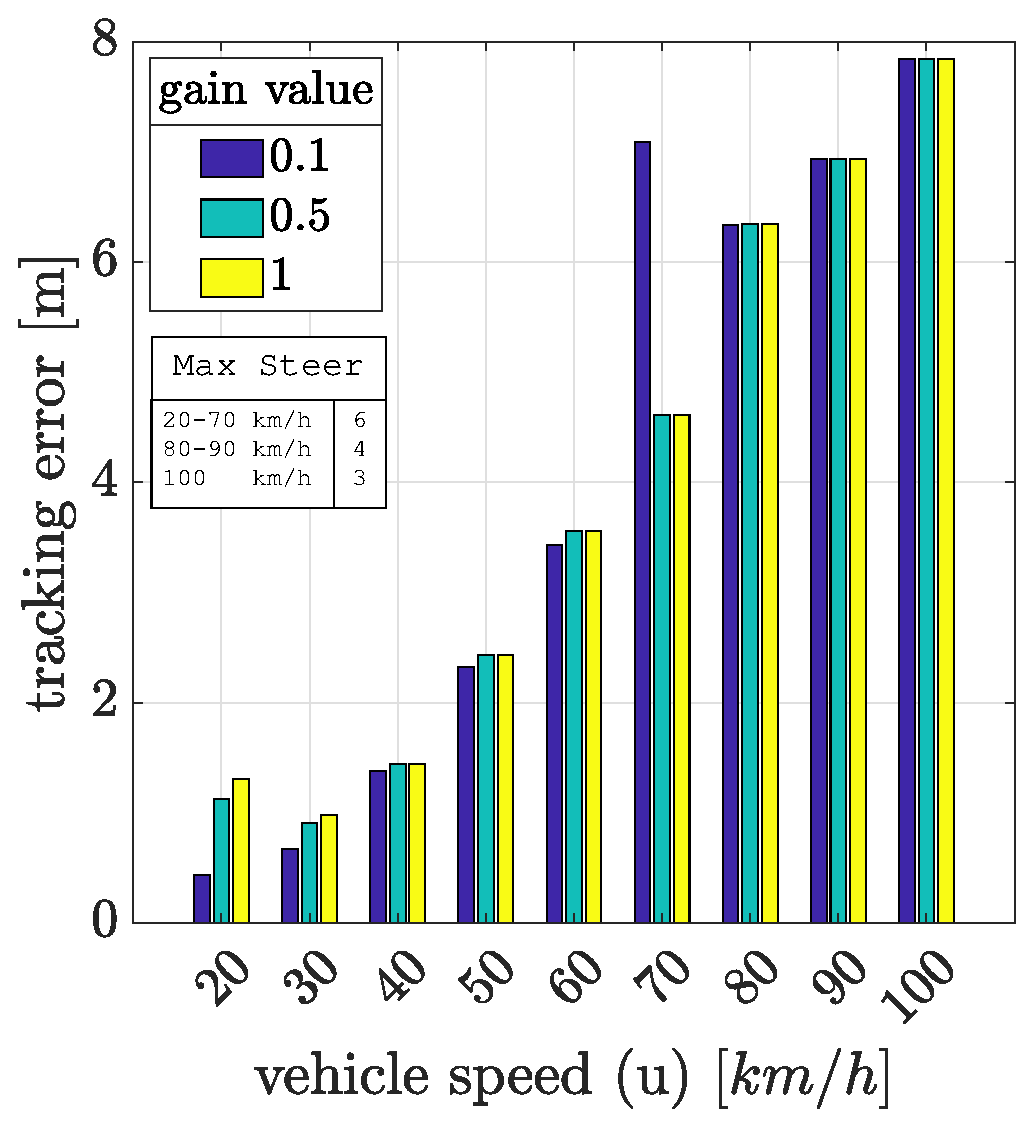
\includegraphics[width=0.5\linewidth]{ex6/q3/ex-63a-3.eps}
        \centering
        \caption{Stanley dynamic lateral controller at different $u$ and gain $\ke$ and $\ky$}
        \label{63a-3}
        \end{figure}


\begin{table}[ht]
    \centering
    \begin{tabular}{c | c| c| c}
      \textbf{$u$ [km/h]}  & \textbf{$\ke$/$\ky$ = 0.1} & \textbf{$\ke$/$\ky$ = 0.5} & \textbf{$\ke$/$\ky$ = 1}\\ \hline
      20 &  \cellcolor{green!10}\num{0.433870147950401} &  \num{1.12319636881579}  &  \num{1.30816540263685}     \\\hline
      40 &  \cellcolor{green!10}\num{1.37630980207272} &  \num{1.43951495823005}  &  \num{1.44215501293828}  \\\hline
      60 &  \cellcolor{green!10}\num{3.43271937243360} &  \num{3.55734662611000} &  \num{3.55734662611000} \\\hline
      80 &  \cellcolor{green!10}\num{6.33232256752558} &  \num{6.34432776705650} &  \num{6.34432776705650} \\\hline
      100 &  \cellcolor{green!10}\num{7.84331899204944} &  \num{7.84331899204944} &  \num{7.84331899204944} \\
    \end{tabular}
    \caption{Tracking error results [Stanley dynamic lateral controller]}
    \label{tab:6.4}
\end{table}


\textbf{Q. Compare the performance of the lateral controllers}


        \begin{figure}[ht!]
        \includegraphics[width=0.5\linewidth]{ex6/q4/ex-64er.eps}
        \centering
        \caption{Lateral controllers maximum tracking error comparison at different $u$}
        \label{64er}
        \end{figure}
   
   
The comparison will be based on the maximum tracking error and the steering behaviour. One example of a low speed (30 km/h) and high speed (70 km/h) run was chosen for each controller. The best performing hyper parameters [look ahead, gains, max steer angle] for each controller were chosen based on the tests previously conducted. The tracking error results are shown in Figure \ref{64er}.

From a tracking error metric prospective, the pure pursuit controller performed the best on both low and high speeds. It was capable of maintaining stability at much higher speeds. As a comparison, pure pursuit was able to achieve target up to 130 km/hr, while the other controllers had trouble with any speed over 70 km/hr. Furthermore, pure pursuit requires only one hyper-parameter to tune.

On the other side of the spectrum, Stanley Kinematic was the worst performer on both low and high speeds. For both the Stanely controllers, it was no surprise they would not perform well, especially on higher speeds due to the lack of a look ahead feature. 

        \begin{figure}[ht]
        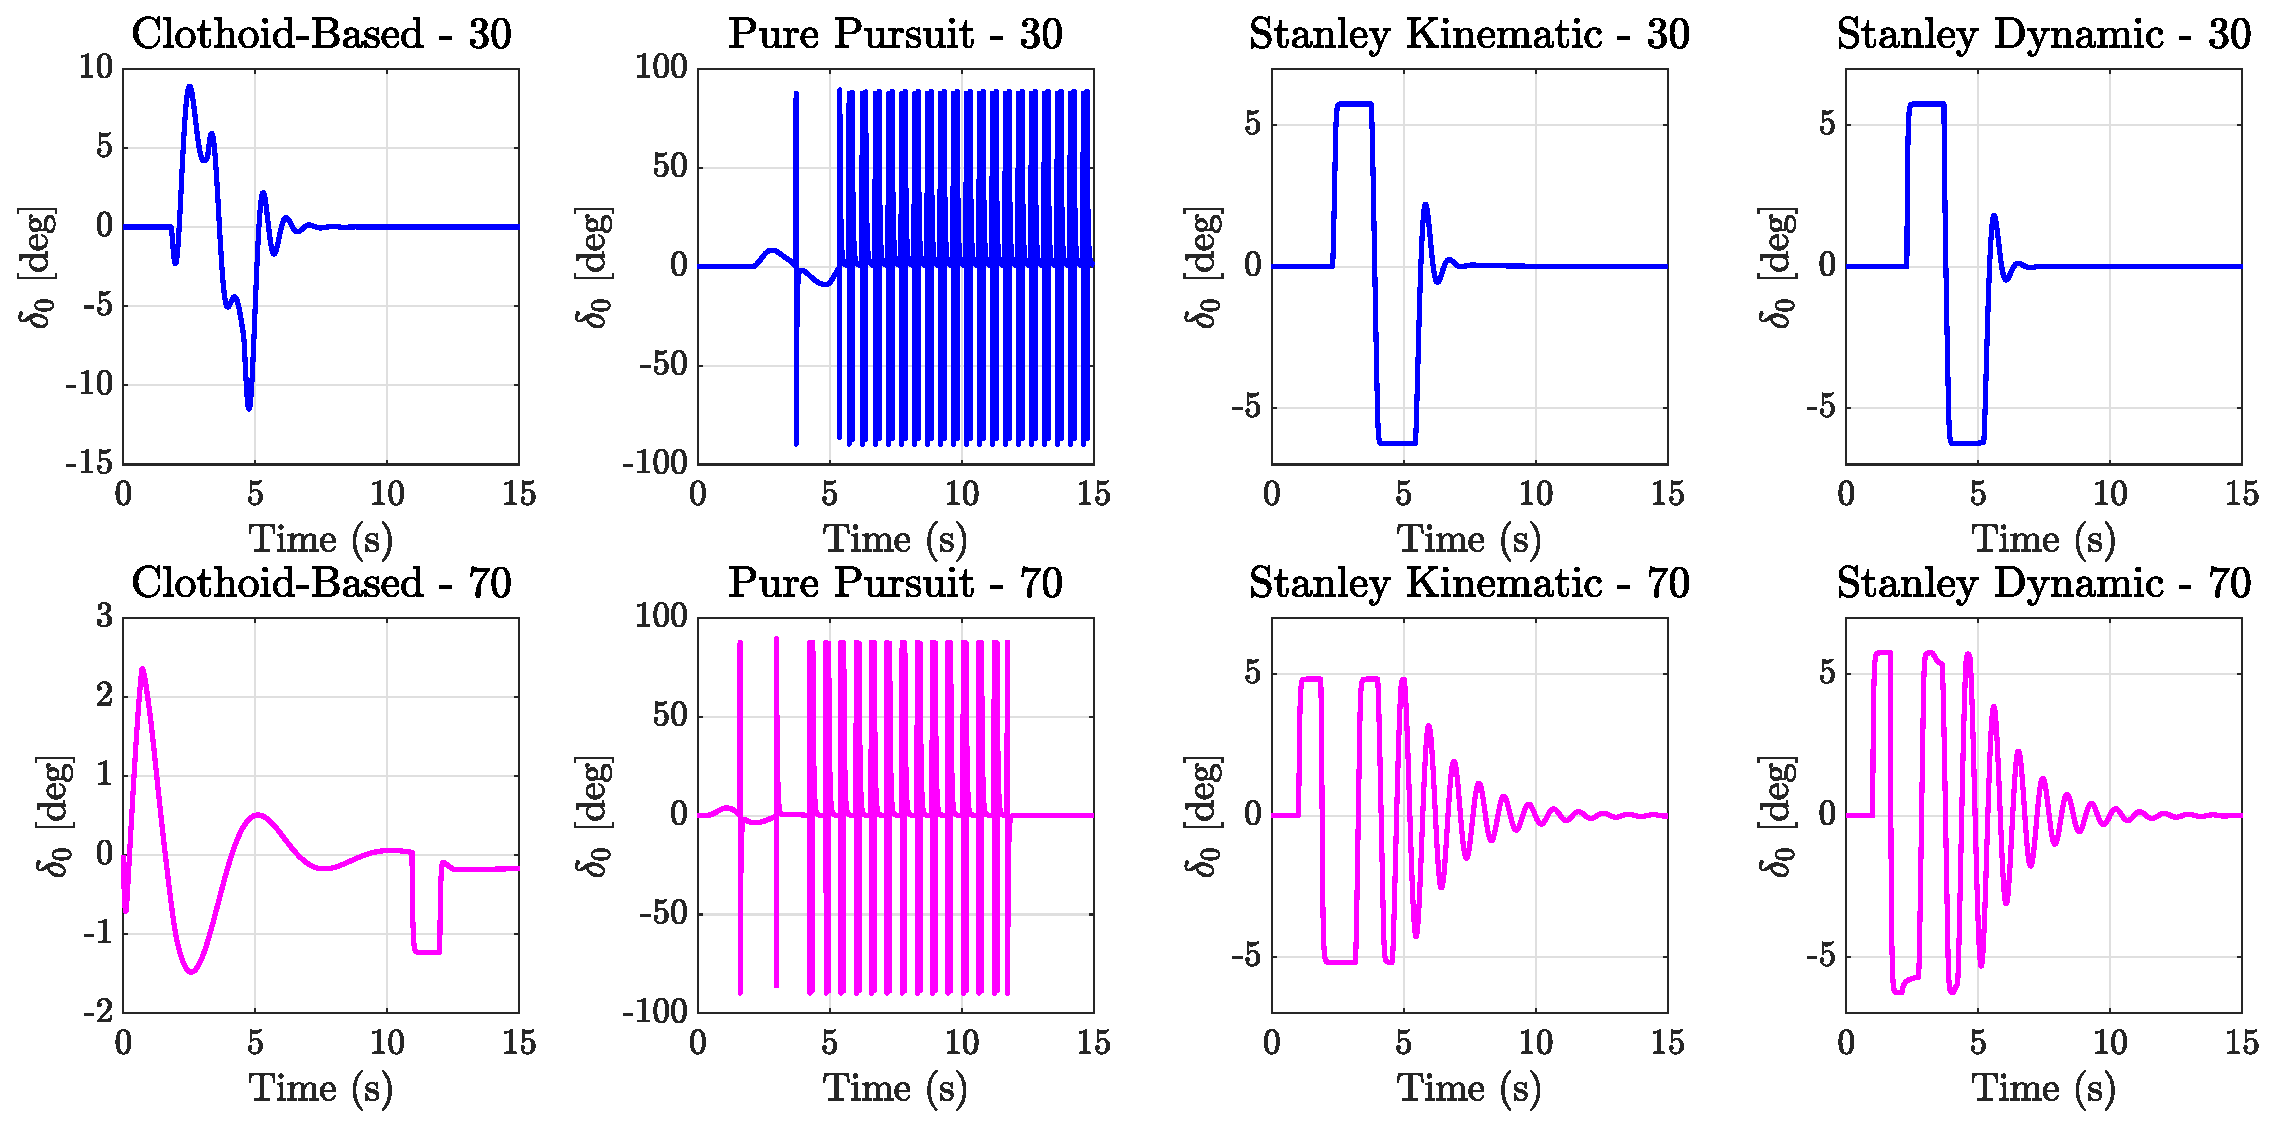
\includegraphics[width=0.99\linewidth]{ex6/q4/ex-64ff.eps}
        \centering
        \caption{Lateral controllers steering behaviour comparison at different $u$}
        \label{64ff}
        \end{figure}
        
The steering angles for the same chosen runs are plotted in Figure \ref{64ff}. The steering angle for pure pursuit exhibited the best smoothness in steering with no sudden jerky changes. It would be a pleasant ride in a vehicle using this controller.   
        
The clothoid based controller is trailing slightly behind pure pursuit as it showed more sudden transitions between angles, which could make it a less comfortable ride compared to the pure pursuit.

Both of the Stanley controllers showed the same pattern. Some oscillation were present at the higher speed run.

Overall, from a tracking error prospective, and steering behaviour, the pure pursuit lateral controller is a clear winner compared to the rest of the controllers tested.

\textbf{Q. Underline the pros and cons of each algorithm}
\begin{table}[ht!]
    \centering
    \begin{tabular}{m{0.14\linewidth}|m{0.39\linewidth}|m{0.39\linewidth}} 
       \textbf{Controller} & \textbf{Pros} & \textbf{Cons} \\
        \hline
        
         Clothoid-based & 
        
    % \begin{minipage}[t]{\linewidth}
    \setlist{leftmargin=*}
    \begin{itemize}[noitemsep]
        \item smooth steering behaviour
        \item benefits from knowledge of the vehicle's handling behaviour
        \item best overall performer at lower speeds
    \end{itemize}
    % \end{minipage} 
    &

    % \begin{minipage}[t]{\linewidth}
    \setlist{leftmargin=*}
    \begin{itemize}[noitemsep]
        \item requires 2 hyper parameters
        \item high computation cost
        \item poor on high speeds

    \end{itemize}
    % \end{minipage} 
    \\ \hline
        
        Pure pursuit & 
        
    % \begin{minipage}[t]{\linewidth}
    \setlist{leftmargin=*}
    \begin{itemize}[noitemsep]
        \item tracks reference very well
        \item simple to implement
        \item only 1 hyper parameter to tune
        \item low computation cost
        \item functions at very high speeds
    \end{itemize}
    % \end{minipage} 
    &

    % \begin{minipage}[t]{\linewidth}
    \setlist{leftmargin=*}
    \begin{itemize}[noitemsep]
        \item look ahead must be specific for each speed
        
    \end{itemize}
    % \end{minipage} 
    \\ \hline
        
        S. kinematic& 
        
    % \begin{minipage}[t]{\linewidth}
    \setlist{leftmargin=*}
    \begin{itemize}[noitemsep]
        \item low computation cost
        \item only 1 hyper parameter
        \item simple to implement
    \end{itemize}
    % \end{minipage}  
    & 

    % \begin{minipage}[t]{\linewidth}
    \setlist{leftmargin=*}
    \begin{itemize}[noitemsep]
        \item no look ahead feature
        \item doesn't do well in high speeds
    \end{itemize}
    % \end{minipage} 
    \\ \hline
        
        S. dynamic & 
        
    % \begin{minipage}[t]{\linewidth}
    \setlist{leftmargin=*}
    \begin{itemize}[noitemsep]
        \item works better on higher speeds than the kinematic version
        \item performs well on low speeds
    \end{itemize}
    % \end{minipage}
    & 

    % \begin{minipage}[t]{\linewidth}
    \setlist{leftmargin=*}
    \begin{itemize}[noitemsep]
        \item no look ahead feature
        \item requires 2 hyper parameters
        \item shows oscillations at higher speeds
    \end{itemize}
    % \end{minipage} 
    \\ 
    \end{tabular}
  \caption{Pros and Cons of lateral controllers}
  \label{tab:6.5}
\end{table}


% \printbibliography %

\end{document}
